% 150 câu đã gỡ khỏi ngân hàng (chuyen_dang) — chép lại vào file dạng để khôi phục

% từ: cau-hoi/lop10/0D0_Xac_suat/0D0-1-3_Dem_phan_tu_khong_gian_mau_bien_co.tex
\begin{ex}%[0D0H1-3]%[ma:85bb8aa7]
	Từ các chữ số $1, 3, 5, 7, 9$ lập được bao nhiêu số  tự nhiên có $5$ chữ số khác nhau mà chữ số đầu tiên là chữ số $3$?
	 \choice
		{$4$ số} 
		 {$6$ số}
		{\True $24$ số} 
		{$12$ số} 
	 \loigiai{
		Số cần lập có dạng $\overline{abcde}$.\\ 
		Chữ số đầu tiên là chữ số $3$ nên $a=3$.\\ 
		Số cách lập $\overline{bcde}$ là $4!=24$.\\ 
		 Vậy lập được tất cả là $1\cdot 24=24$ số.
	} 
\end{ex}

% từ: cau-hoi/lop10/0D1_Menh_de_Tap_hop/0D1-1-2_Tinh_dung_sai_cua_menh_de.tex
\begin{ex}%[0D1N1-2]%[ma:0f915a99]
	Cho tứ giác $ABCD$ có $\overrightarrow{AD}=\overrightarrow{BC}$. Mệnh đề nào trong các mệnh  đề sau là \textbf{sai}?
	 \choice
		{Tứ  giác $ABCD$ là hình bình hành}
		{$DA=BC$} 
		{\True $\overrightarrow{AC}=\overrightarrow{BD}$} 
		 {$\overrightarrow{AB}=\overrightarrow{DC}$}
	 \loigiai{
	\immini 
		{$AC$ và $BD$ là hai đường chéo của tứ giác $ABCD$ nên hai vectơ $\overrightarrow{AC}$, $\overrightarrow{BD}$ không cùng phương  vì vậy không thể bằng nhau.}
		 {
		\begin{tikzpicture}[scale=1,line join=round,line cap=round,font=\footnotesize,>=stealth]
				 \def\d{4}
				\def\r{3} 
				\path (0:0) coordinate (B) 
					++(0:\d)  coordinate (C)
					++(50:\r) coordinate (D) 
					($(B)+(D)-(C)$) coordinate (A); 
				 \draw (A)--(B)--(C)--(D)--cycle;
				\foreach \x/ \goc  in {A/180,B/180,C/0,D/0}
				\fill (\x) circle (1pt) 
					 ($(\x)+(\goc:3mm)$) node {$\x$};
			\end{tikzpicture}
		 }
	 }
\end{ex}

% từ: cau-hoi/lop10/0D1_Menh_de_Tap_hop/0D1-1-2_Tinh_dung_sai_cua_menh_de.tex
\begin{ex}%[0D1H1-2]%[ma:a9f2f580]
	Cho tứ giác $ABCD$. Gọi $M$, $N$, $P$ lần lượt  là trung điểm của $AD$, $BC$ và $AC$. Biết $\overrightarrow{MP}=\overrightarrow{PN}$. Chọn câu \textbf{đúng}.
	 \choice
		 {$\overrightarrow{AC}=\overrightarrow{BD}$}
		 {$\overrightarrow{AC}=\overrightarrow{BC}$}
		{\True $\overrightarrow{AD}=\overrightarrow{BC}$} 
		{$\overrightarrow{AD}=\overrightarrow{BD}$} 
	 \loigiai{
		\begin{center}
			\begin{tikzpicture}[scale=1,line join=round,line cap=round,font=\footnotesize,>=stealth]
					\def\d{4} 
					 \def\r{3}
					 \path (0:0) coordinate (B)
						 ++(0:\d) coordinate (C)
						++(70:\r)  coordinate (D)
						($(B)+(D)-(C)$) coordinate  (A)
						($(A)!0.5!(C)$) coordinate (P) 
						 ($(B)!0.5!(C)$) coordinate (N)
						($(A)!0.5!(D)$)  coordinate (M);
					\draw  (A)--(B)--(C)--(D)--cycle (A)--(C);
					\foreach  \x/ \goc in {A/180,B/180,C/0,D/0,M/90,N/-90,P/90}
					\fill  (\x) circle (1pt)
						($(\x)+(\goc:3mm)$)  node {$\x$};
				\end{tikzpicture}
		\end{center}
		Ta có $MP \parallel DC$, $MP=\dfrac{1}{2}DC$, $PN//AB$, $PN=\dfrac{1}{2}AB$.\\ Mà $MP=PN \Rightarrow\overrightarrow{AB}=\overrightarrow{DC}\Rightarrow  ABCD$ là hình bình hành $\Rightarrow\overrightarrow{AD}=\overrightarrow{BC}$.
	 }
\end{ex}

% từ: cau-hoi/lop10/0D1_Menh_de_Tap_hop/0D1-3-1_Giao_va_hop_cua_hai_tap_hop_roi_rac.tex
\begin{ex}%[0D1Y3-1]%[ma:d4414e61]
	Cho dãy số liệu $1; 3; 4; 6; 8; 9; 11$.  Số trung bình cộng của dãy số liệu trên?
	 \choice
		 {$ 11 $}
		{\True  $ 6 $ }
		{$ 9 $} 
		{$  5 $}
	\loigiai{ 
		Số  trung bình cộng của dãy số liệu trên là $ \overline{x}=\dfrac{1+3+4+6+8+9+11}{7}= 6$.
	 }
\end{ex}

% từ: cau-hoi/lop10/0D1_Menh_de_Tap_hop/0D1-3-1_Giao_va_hop_cua_hai_tap_hop_roi_rac.tex
\begin{ex}%[0D1Y3-1]%[ma:5c4f8a9d]
	Lớp $ 10C $ của một trường trung học phổ thông có điểm thi môn Toán được cho dưới bảng sau 
	\begin{center}
		\begin{tabular}{|l|c|c|c|c|c|c|}
			\hline Điểm thi & 5 &  6 & 7 & 8 & 9 & 10 \\
			 \hline Tần số & 5 & 7 & 12 & 14 & 3 & 4 \\
			\hline 
		\end{tabular}
	\end{center}
	Tính điểm trung  bình cộng môn Toán của lớp $10C$ (làm tròn đến hàng phần mười)?
	 \choice
		{$  8 $}
		{$ 7,5 $  }
		 {$ 7,6 $}
		{\True  $ 7,3 $}
	\loigiai{ 
		Điểm trung bình của lớp $  10 C $ là
		$ \overline{x}=\dfrac{5\cdot 5+7\cdot 6+12\cdot 7+14\cdot 8+3\cdot 9+4\cdot10}{45} \approx 7,3$. 
	} 
\end{ex}

% từ: cau-hoi/lop10/0D1_Menh_de_Tap_hop/0D1-3-2_Hieu_va_phan_bu_cua_hai_tap_hop_roi_rac.tex
\begin{ex}%[0D1Y3-2]%[ma:8f1f3566]
	Cho dãy số liệu $1; 2; 7; 5; 10; 9; 8$. Số trung vị của  dãy trên bằng bao nhiêu?
	 \choice
		{$ 7  $}
		{\True  $ 6 $}
		{$  8 $}
		{$  2 $ }
	\loigiai{ 
		Xắp xếp mẫu số liệu theo thứ tự  không giảm $1; 2; 5; 7; 8; 9; 10$.\\
		Do  đó trung vị của mẫu số liệu $ M_e=\dfrac{5+7}{2}=6$.
	} 
\end{ex}

% từ: cau-hoi/lop10/0D1_Menh_de_Tap_hop/0D1-3-4_Hieu_va_phan_bu_dung_doan_khoang.tex
\begin{ex}%[0D1H3-4]%[ma:bc823e38]
	Cho tam giác $ABC$ có $AB=4$, $AC=3$ và $\widehat{BAC}=60^{\circ}$. (Kết quả làm  tròn đến hàng đơn vị).
	\choiceTF {\True  $BC=\sqrt{13}$}{ $\widehat{ABC}\approx75^{\circ}$}{ $\widehat{ACB}\approx45^{\circ}$}{\True $AB$ là cạnh có độ dài lớn nhất trong tam giác}
	\loigiai{ 
		\begin{itemchoice}
			\itemch Áp  dụng định lí Côsin: $BC^{2}=4^{2}+3^{2}-2\cdot4\cdot3\cdot\cos 60^{\circ}=16+9-12=13$. Do đó $BC=\sqrt{13}$.
			\itemch Áp dụng định lí Côsin: $\cos B=\dfrac{AB^{2}+BC^{2}-AC^{2}}{2AB\cdot BC}=\dfrac{4^{2}+13-3^{2}}{2\cdot4\cdot\sqrt{13}}=\dfrac{20}{8\sqrt{13}}=\dfrac{5\sqrt{13}}{26}$. Do  đó $\widehat{ABC}\approx46^{\circ}$.
			 \itemch $\widehat{ACB}=180^\circ-\widehat{BAC}-\widehat{ABC}\approx180^\circ-60^\circ-46^\circ\approx74^\circ$.
			\itemch Ta có $AB=4$, $AC=3$, $BC=\sqrt{13}\approx3{,}6$. Cạnh lớn nhất là  $AB=4$.
		\end{itemchoice}
	} 
\end{ex}

% từ: cau-hoi/lop10/0D3_Ham_so_bac_hai_va_do_thi/0D3-1-1_Xac_dinh_mot_ham_so.tex
\begin{ex}%[0D3Y1-1]%[ma:f2b2f671]
	Gieo một con súc sắc, số phần tử  của không gian mẫu là
	 \choice
		 {$24$}
		 {$12$}
		{$8$} 
		{\True $6$} 
	\loigiai{ 
		Ta có $n(\Omega)=6$. 
	 }
\end{ex}

% từ: cau-hoi/lop10/0D3_Ham_so_bac_hai_va_do_thi/0D3-1-2_Tap_xac_dinh_cua_ham_so.tex
\begin{ex}%[0D3N1-2]%[ma:2a9bfbb1]
	Miền nghiệm của hệ bất phương trình $\heva{& x-2y+2>0\\ & 2x+y>3 }$ là phần  mặt phẳng chứa điểm
	 \choice
		{$\left(1;1\right)$ } 
		 {$\left(-1;2\right)$}
		{$\left(2;-1\right)$} 
		{\True $\left(2;1 \right)$} 
	 \loigiai{
		Lần lượt thay các bộ số vào hệ bất phương trình ta được một nghiệm của hệ bất phương trình trên là $\left(2;1\right)$. 
	 }
\end{ex}

% từ: cau-hoi/lop10/0D3_Ham_so_bac_hai_va_do_thi/0D3-1-2_Tap_xac_dinh_cua_ham_so.tex
\begin{ex}%[0D3B1-2]%[ma:f50d3c23]
	Không gian mẫu của phép thử ``\textit{gieo một con súc sắc $6$  mặt hai lần liên tiếp}'' có bao nhiêu phần tử?
	 \choice
		 {$12$}
		{\True  $36$}
		{$24$} 
		 {$30$}
	 \loigiai{
		Phép thử ``\textit{gieo một con súc sắc $6$ mặt  hai lần liên tiếp}'' có $6^2=36$ phần tử.
	} 
\end{ex}

% từ: cau-hoi/lop10/0D3_Ham_so_bac_hai_va_do_thi/0D3-1-3_Gia_tri_cua_ham_so.tex
\begin{bt}%[0D3N1-3]%[ma:64612ca4]
	Biểu thức $L=y-x$, với $x$ và $y$ thỏa mãn hệ bất phương trình $\heva{&2x+3y-6 \leq 0\\&x\geq 0\\&2x-3y-1\leq 0}$, đạt giá trị lớn  nhất
	là $a$ và đạt giá trị nhỏ nhất là $b$. Khi đó $a+12b$ bằng  bao nhiêu?
	\shortans{-9} 
	\loigiai{ 
		Trước hết, ta vẽ ba  đường thẳng $d_1: 2x+3y-6=0$, $d_2:x=0$, $d_3: 2x-3y-1=0$.
		\begin{center}
			\begin{tikzpicture}[line join=round,line cap=round,>=stealth,font=\footnotesize,scale=0.6]
					\draw (0,0) node [above  left] {$O$};
					\draw [->] (-3.5,0)--(3.5,0) node[below]{$x$}; 
					\draw[->] (0,-3.5)--(0,3.5) node[left]{$y$}; 
					\clip (-3.5,-3.5) rectangle  (3.5,3.5);
					\draw[samples=100,smooth,domain=-3.5:3.5,black] plot  (\x,{-(2/3)*(\x)+2});
					 \draw[samples=100,smooth,domain=-3.5:3.5,black] plot (\x,{(2/3)*(\x)-(1/3)});
					 \fill[pattern=north east lines,opacity=0.6] plot[domain=-3.5:3.5](\x,{-(2/3)*(\x)+2})--plot[domain=3.5:-3.5](\x,{3.5})--cycle;
					\fill[pattern=north  east lines,opacity=0.6] plot[domain=-3.5:3.5](\x,{(2/3)*(\x)-(1/3)})--plot[domain=3.5:-3.5](\x,{-3.5})--cycle;
					\fill[pattern=north  east lines,opacity=0.6] (-3.5,-3.5)--(0,-3.5)--(0,3.5)--(-3.5,3.5)--cycle;
					\node[right] at (0,2) {$A$}; 
					\path  (0,2) node[left]{$2$};
					\node[below] at (7/4,5/6) {$B$}; 
					\draw[dashed](7/4,0) node[below]{$\tfrac{7}{4}$; 
						$\tfrac{7}{4}$}--(7/4,5/6)--(0,5/6)  node[left]{$\tfrac{5}{6}$};
					\node[right]  at (0,-1/3) {$C$};
					\path  (0,-1/3) node[left]{$\tfrac{-1}{3}$};
				\end{tikzpicture}
		\end{center}
		Ta thấy $\left(0;0\right)$ là nghiệm của cả ba bất phương trình. Điều đó có nghĩa gốc tọa độ thuộc cả ba miền nghiệm của cả ba bất phương trình. Sau khi gạch bỏ các miền không thích hợp, miền không bị gạch là miền nghiệm  của hệ (kể cả biên).
		Miền nghiệm là hình  tam giác $ABC$ (kể cả biên), với $A\left(0;2\right)$, $B\left(\dfrac{7}{4};\dfrac{5}{6}\right)$, $C\left(0;-\dfrac{1}{3}\right)$.\\
		Ta có $L\left(A\right)=L\left(2;0\right)=2-0=2$,\\  $L\left(B\right)=L\left(\dfrac{7}{4};\dfrac{5}{6} \right)=\dfrac{6}{5}-\dfrac{7}{4}=-\dfrac{11}{12}$,\\ $L\left(C\right)=L\left(0;-\dfrac{1}{3} \right)=-\dfrac{1}{3}-0=-\dfrac{1}{3}$.\\
		Vậy $a=2$,  $b=-\dfrac{11}{12}$.\\
		 Khi đó $a+12b=-9$.
	 }
\end{bt}

% từ: cau-hoi/lop10/0D3_Ham_so_bac_hai_va_do_thi/0D3-1-5_Tinh_dong_bien_nghich_bien.tex
\begin{bt}%[0D3H1-5]%[ma:c2a2e793]
	Biểu diễn tập nghiệm của hệ bất phương trình sau trên mặt phẳng toạ độ $Oxy$? $$\heva{& 2 x+y -2>0 \\& -3x+  y-4 <0.}$$
	 \loigiai{
		\begin{itemize}
			\item Vẽ đường thẳng $\Delta_1\colon 2x+y-2=0$ đi qua hai điểm $\left(0;2\right)$ và $\left(1;0\right)$ và đường thẳng  $\Delta_2\colon -3x+y-4=0$ đi qua hai điểm $\left(0;4\right)$ và $\left(-\dfrac{4}{3};0\right)$.
			\item Xét điểm  $O(0; 0)\notin \Delta_1$. Ta có $2\cdot 0 +0 -2 =-2 <0$. Suy ra, miền nghiệm của bất phương trình $2x+y-2>0$ là nửa mặt phẳng bờ $\Delta_1$ chứa điểm $O$ không kể đường thẳng $\Delta_1$.
			\item Xét điểm $O(0; 0)\notin \Delta_2$. Ta có $-3\cdot 0 +0 -4 =-4 <0$. Suy ra, miền nghiệm của bất phương trình $-3x+y-4<0$ là nửa mặt phẳng bờ $\Delta_2$ chứa điểm $O$ không kể  đường thẳng $\Delta_2$.
		\end{itemize}
		\begin{center}
			\begin{tikzpicture}[scale=0.6,thick,>=stealth']
					\draw[->] (-3,0) --  (4,0) node[above]{$x$};
					\foreach \x  in {1,2,3}
					\draw[shift={(\x,0)},color=black] (0pt,2pt) -- (0pt,-2pt) node[below] {\footnotesize $\x$}; 
					\draw[->,color=black]  (0,-2) -- (0,6) node[right]{$y$};
					\foreach  \y in {1,2,3,4,5}
					\draw[shift={(0,\y)},color=black] (2pt,0pt)  -- (-2pt,0pt) node[left] {\footnotesize $\y$};
					\node[below  left] at (0,0) {$O$};
					\clip  (-3,-2) rectangle (4,6);
					\draw[line width=1.2pt,smooth,samples=100,domain=-3:9]  plot (\x,{-2*(\x)+2});
					\draw[line  width=1.2pt,smooth,samples=100,domain=-3:7] plot (\x,{3*(\x)+4});
					\fill[pattern=north east lines]  (-3,8)--(7,8) --(7,-12)--(2,-2)-- cycle;
					\fill[pattern=north east lines] (-3,8)--(4/3,8)  --(-2,-2)--(-3,-2)-- cycle;
				\end{tikzpicture}
		\end{center}
	 }
\end{bt}

% từ: cau-hoi/lop10/0D3_Ham_so_bac_hai_va_do_thi/0D3-2-1_Xac_dinh_ham_so_bac_hai.tex
\begin{ex}%[0D3Y2-1]%[ma:58b9c20c]
	Trong các biểu thức dưới đây, biểu thức nào là  một tam thức bậc hai?
	 \choice
		{\True $f(x)=x^2+3$} 
		{$f(x)=0 x^2+2  x$}
		{$f(x)=\dfrac{1}{x^2}$} 
		{$f(x)=2 x+1$} 
	 \loigiai{
		Trong các biểu thức trên, $f(x)=x^2+3$ là một  tam thức bậc hai.
	} 
\end{ex}

% từ: cau-hoi/lop10/0D3_Ham_so_bac_hai_va_do_thi/0D3-2-1_Xac_dinh_ham_so_bac_hai.tex
\begin{ex}%[0D3Y2-1]%[ma:6d3cba2d]
	Biểu thức nào sau đây là một  tam thức bậc hai?
	\choice 
		{$f(x)=x^4-2x^2+2023$} 
		{\True $f(x)=\sqrt{2}x^2-2x+2023$} 
		 {$f(x)=\left(\dfrac{1}{x}\right)^2-\dfrac{2}{x}-3$}
		{$f(x)=x+3\sqrt{x}-2023$} 
	 \loigiai{
		Tam thức bậc hai có dạng $y=ax^2+bx+c$ với $a\ne  0$.\\
		Do đó, $f(x)=\sqrt{2}x^2-2x+2023$ là một tam  thức bậc hai.
	 }
\end{ex}

% từ: cau-hoi/lop10/0D3_Ham_so_bac_hai_va_do_thi/0D3-2-2_Bang_bien_thien_tinh_don_dieu_max_min.tex
\begin{ex}%[0D3Y2-2]%[ma:49f74143]
	Bảng xét dấu 
	\begin{center}
		
\begin{tikzpicture}
				 \tkzTabInit[nocadre=false,lgt=1.1,espcl=1.8,deltacl=0.5]
					 {$x$/.7,$f (x)$/.7}
					 {$-\infty$,$1$,$3$,$+\infty$}
				\tkzTabLine{,-,$0$,+,$0$,-} 
			\end{tikzpicture}
	\end{center}
	là của tam thức bậc hai nào dưới đây? 
	\choice 
		 {\True $f(x)=-x^2 +4x -3$}
		{$f(x)=x^2  -4x +3$}
		{$f(x)=-x^2  +x -3$}
		{$f(x)=-x^2  +4x $}
	\loigiai{Từ bảng xét dấu suy ra hệ số $a<0$, nghiệm của biểu thức là $x=1$ hoặc $x=3$. Do đó $f(x)=-x^2 +4x -3$. 
	} 
\end{ex}

% từ: cau-hoi/lop10/0D3_Ham_so_bac_hai_va_do_thi/0D3-2-2_Bang_bien_thien_tinh_don_dieu_max_min.tex
\begin{ex}%[0D3N2-2]%[ma:72d65c94]
	Khẳng định nào sau  đây về hàm số $y=x^2$ là khẳng định đúng?
	\choice 
		{Hàm  số nghịch biến trên $\mathbb{R}$}
		{Hàm số đồng biến  trên $\mathbb{R}$}
		{Hàm số nghịch biến trên  $[0;+\infty)$}
		{\True Hàm  số đồng biến trên $[0;+\infty)$}
	\loigiai{ 
		Hàm số $y=x^2$ có hệ số $a=1>0$ nên hàm đồng biến trên $\left(-\dfrac{b}{2a};+\infty \right) $ hay $[0;+\infty)$ (vì hàm số chỉ bằng $0$  tại một điểm là $x=0$).
	 }
\end{ex}

% từ: cau-hoi/lop10/0D3_Ham_so_bac_hai_va_do_thi/0D3-2-2_Bang_bien_thien_tinh_don_dieu_max_min.tex
\begin{ex}%[0D3N2-2]%[ma:4957d7b6]
	Cho hàm số $y=  2x^2-4x+1$. Các khẳng định sau đây đúng hay sai?
	 \choiceTF
		 {Hàm số đồng biến trên $(0;+\infty)$}
		{Hàm số nghịch biến trên $(-\infty; 2)$} 
		{\True Hàm số  đồng biến trên $(2;+\infty)$}
		 {\True Hàm số nghịch biến trên $(-\infty;0)$}
	 \loigiai{
		Ta có $a=2 >0$; $-\dfrac{b}{2a} =1$, nên hàm  số
		\begin{itemize}
			\item Hàm số đồng biến  trên $(1;+\infty)$;
			\item Hàm số nghịch biến  trên $(-\infty;1)$.
		\end{itemize}
		Suy  ra
		\begin{itemchoice}
			\itemch Hàm  số không đồng biến trên $(0;+\infty)$.
			 \itemch Hàm số không nghịch biến trên $(-\infty; 2)$.
			 \itemch Hàm số đồng biến trên $(2;+\infty) \subset (1;+\infty)$.
			\itemch Hàm số nghịch  biến trên $(-\infty;0) \subset (-\infty;1)$.
		\end{itemchoice}
	} 
\end{ex}

% từ: cau-hoi/lop10/0D3_Ham_so_bac_hai_va_do_thi/0D3-2-2_Bang_bien_thien_tinh_don_dieu_max_min.tex
\begin{bt}%[0D3C2-2]%[Nguyễn Đức Tuệ]%[ma:59153f09]
	Hãy tìm tất cả các giá trị của tham số $m$ để hàm số $y=-x^2+(2m-3)x+1$ đồng biến trên khoảng $(-\infty; -5)$.
	\loigiai{
		Tập xác định $\mathscr{D}=\mathbb{R}$.\\
		Ta có hoành độ đỉnh $x=-\dfrac{b}{2a}=\dfrac{2m-3}{2}$.\\
		Do $a=-1<0$ nên ta có bảng biến thiên như sau
		\begin{center}
			
\begin{tikzpicture}[line width=0.9pt]
				\tkzTabInit[lw=1,lgt=1.2,espcl=2.5,deltacl=0.6]
				{$x$/1.2,$y$/2}
				{$-\infty$,$\dfrac{2m-3}{2}$,$+\infty$}
				\tkzTabVar{-/$-\infty$,+/,-/$-\infty$}
			\end{tikzpicture}
		\end{center}
		Dựa vào bảng biến thiên suy ra hàm số đồng biến trên khoảng $(-\infty; -5)$ khi và chỉ khi $$\dfrac{2m-3}{2}\ge -5\Leftrightarrow m\ge -\dfrac{7}{2}.$$
		Vậy $m\ge -\dfrac{7}{2}$.
	}
\end{bt}

% từ: cau-hoi/lop10/0D7_Bat_phuong_trinh_bac_2_mot_an/0D7-2-2_Giai_bat_phuong_trinh_bac_hai_biet_BXD_do_thi.tex
\begin{ex}%[0D7H2-2]%[ma:f645a8c3]
	\immini{Cho hàm số $f(x)=ax^2+bx+c$  có đồ thị như hình bên.
	\choiceTF 
		 {Hàm số đồng biến trên $(1;3)$}
		{Phương  trình $f(x)=0$ vô nghiệm}
		{\True Trục đối xứng của đồ thị hàm số có  phương trình $x=2$}
		{\True $f(x)<0\Leftrightarrow  x \in (1;3)$}
		 }{
		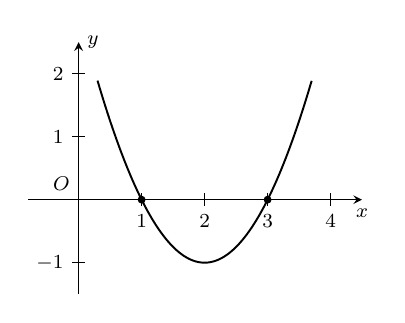
\begin{tikzpicture}[smooth,samples=300,scale=0.8,>=stealth,font=\footnotesize]
				 \draw[->] (-0.8,0)--(4.5,0) node[below]{$x$};
				\draw[->] (0,-1.5)--(0,2.5) node[right]{$y$}; 
				 \draw (0,0) node[above left]{$O$};
				\draw[line  width=0.7pt,domain=0.3:3.7] plot (\x,{(\x)^2-4*(\x)+3});
				\draw[fill=black] (1,0) circle (1.5pt) 
					(3,0)  circle (1.5pt);
				\foreach \x  in {1,2,3,4}\draw (\x,0.1)--(\x,-0.1) node [below] {\footnotesize $\x$};
				\foreach \y in {-1,1,2}\draw (0.1,\y)--(-0.1,\y) node [left]  {\footnotesize $\y$};
			\end{tikzpicture}
		 }
	 \loigiai{
		\begin{itemchoice}
			\itemch Sai. Vì hàm số  đồng biến trên các khoảng $(-\infty;1)$ và $(3;+\infty)$.
			\itemch Sai. Vì phương trình có hai nghiệm  $x=1$ hoặc $x=3$.
			\itemch Đúng. Vì trục đối xứng của đồ thị hàm số có  phương trình $x=2$.
			\itemch Đúng. Vì $f(x)<0$  thì $1<x<3$.
		\end{itemchoice}
	 }
\end{ex}

% từ: cau-hoi/lop10/0D7_Bat_phuong_trinh_bac_2_mot_an/0D7-2-2_Giai_bat_phuong_trinh_bac_hai_biet_BXD_do_thi.tex
\begin{bt}%[0D7H2-2]%[Tex hóa SGK CD-CT,T7/22, Phạm Tiến Long]%[ma:600f9b5d]
	Dựa vào đồ thị của hàm số bậc hai đã cho, hãy nêu tập nghiệm của các bất phương trình bậc hai tương ứng.
	\begin{center}
		\begin{tikzpicture}[scale=0.7, font=\footnotesize, line join=round, line cap=round, >=stealth]
			\def\ymin{-1} \def\ymax{3.5}
			\def\xmin{-3} \def\xmax{2} 
			\draw[->] (\xmin,0)--(\xmax,0) node [below]{$x$};
			\draw[->] (0,\ymin)--(0,\ymax) node [left]{$y$};
			\fill (0,0)circle(1pt)node[above left]{$O$} (-5/2,0)circle(1pt)node[above left]{$-\dfrac{7}{3}$}
			(1,0)circle(1pt)node[above right]{$1$};
			\draw (-0.9,3.5)node[above]{a) $f(x)\ge 0$} (-3.6,-0.5)node{ $y=f(x)$};
			\clip (\xmin+0.1,\ymin+0.1) rectangle (\xmax-0.1,\ymax-0.1);
			\draw[smooth,samples=300] plot(\x,{-((\x)+5/2)*((\x)-1)});
		\end{tikzpicture}
		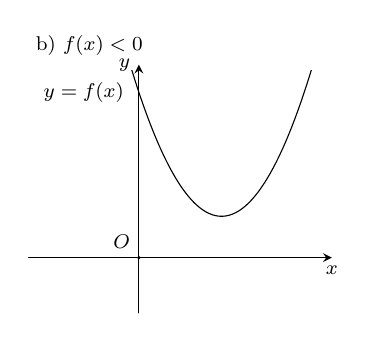
\begin{tikzpicture}[scale=0.7, font=\footnotesize, line join=round, line cap=round, >=stealth]
			\def\ymin{-1} \def\ymax{3.5}
			\def\xmin{-2} \def\xmax{3.5} 
			\draw[->] (\xmin,0)--(\xmax,0) node [below]{$x$};
			\draw[->] (0,\ymin)--(0,\ymax) node [left]{$y$};
			\fill (0,0)circle(1pt)node[above left]{$O$};
			\draw (-0.9,3.5)node[above]{b) $f(x)< 0$} (-1,3)node{ $y=f(x)$};
			\clip (\xmin+0.1,\ymin+0.1) rectangle (\xmax-0.1,\ymax-0.1);
			\draw[smooth,samples=300] plot(\x,{((\x)-2)^2+\x-1});
		\end{tikzpicture}
		\begin{tikzpicture}[scale=0.7, font=\footnotesize, line join=round, line cap=round, >=stealth]
			\def\ymin{-1} \def\ymax{3.5}
			\def\xmin{-1} \def\xmax{7} 
			\draw[->] (\xmin,0)--(\xmax,0) node [below]{$x$};
			\draw[->] (0,\ymin)--(0,\ymax) node [left]{$y$};
			\fill (0,0)circle(1pt)node[above left]{$O$} (3,0)circle(1pt)node[below left]{$3$}
			(4,0)circle(1pt)node[below right]{$4$};
			\draw (0,3.5)node[above]{c) $f(x)> 0$} (3,3)node{ $y=f(x)$};
			\draw[smooth,samples=300,domain=1.6:5.3] plot(\x,{\x^2-7*\x+12});
		\end{tikzpicture}
	\end{center}
	\begin{center}
		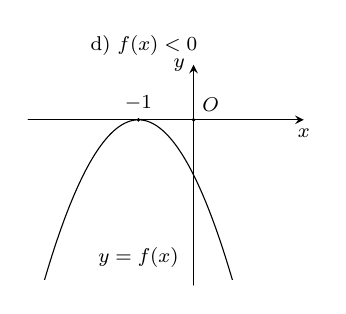
\begin{tikzpicture}[scale=0.7, font=\footnotesize, line join=round, line cap=round, >=stealth]
			\def\ymin{-3} \def\ymax{1}
			\def\xmin{-3} \def\xmax{2} 
			\draw[->] (\xmin,0)--(\xmax,0) node [below]{$x$};
			\draw[->] (0,\ymin)--(0,\ymax) node [left]{$y$};
			\fill (0,0)circle(1pt)node[above right]{$O$} (-1,0)circle(1pt)node[above]{$-1$};
			\draw (-0.9,1)node[above]{d) $f(x)< 0$} (-1,-2.5)node{ $y=f(x)$};
			\clip (\xmin+0.1,\ymin+0.1) rectangle (\xmax-0.1,\ymax-0.1);
			\draw[smooth,samples=300] plot(\x,{-(\x+1)^2});
		\end{tikzpicture}
		\begin{tikzpicture}[scale=0.7, font=\footnotesize, line join=round, line cap=round, >=stealth]
			\def\ymin{-1.3} \def\ymax{2.5}
			\def\xmin{-1} \def\xmax{5} 
			\draw[->] (\xmin,0)--(\xmax,0) node [below]{$x$};
			\draw[->] (0,\ymin)--(0,\ymax) node [left]{$y$};
			\fill (0,0)circle(1pt)node[above right]{$O$} (5/2,0)circle(1pt)node[below]{$\dfrac{5}{2}$};
			\draw (0,2.6)node[above]{e) $f(x)\le 0$} (2.2,2.5)node{ $y=f(x)$};
			\clip (\xmin+0.1,\ymin+0.1) rectangle (\xmax-0.1,\ymax-0.1);
			\draw[smooth,samples=300] plot(\x,{(\x-5/2)^2});
		\end{tikzpicture}
		\begin{tikzpicture}[scale=0.7, font=\footnotesize, line join=round, line cap=round, >=stealth]
			\def\ymin{-1.5} \def\ymax{2.5}
			\def\xmin{-1} \def\xmax{5} 
			\draw[->] (\xmin,0)--(\xmax,0) node [below]{$x$};
			\draw[->] (0,\ymin)--(0,\ymax) node [left]{$y$};
			\fill (0,0)circle(1pt)node[above right]{$O$} (3/2,0)circle(1pt)node[below left]{$\dfrac{3}{2}$}
			(7/2,0)circle(1pt)node[below right]{$\dfrac{7}{2}$};
			\draw (0,2.5)node[above]{f) $f(x)\ge 0$} (2,2)node{ $y=f(x)$};
			\clip (\xmin+0.1,\ymin+0.1) rectangle (\xmax-0.1,\ymax-0.1);
			\draw[smooth,samples=300] plot(\x,{(\x-3/2)*(\x-7/2)});
		\end{tikzpicture}
	\end{center}
	\loigiai{
		\begin{multicols}{3}
			\begin{enumerate}[a)]
				\item $\left[-\dfrac{7}{3};1\right]$;
				\item $\varnothing$;
				\item $(-\infty;3) \cup (4;+\infty)$;
				\item $\mathbb{R} \setminus \{-1\}$;
				\item $\left\{\dfrac{5}{2}\right\}$;
				\item $\left(-\infty;\dfrac{3}{2}\right] \cup \left[\dfrac{7}{2};+\infty \right)$.
			\end{enumerate}
		\end{multicols}
	}
\end{bt}

% từ: cau-hoi/lop10/0D7_Bat_phuong_trinh_bac_2_mot_an/0D7-3-6_Toan_hinh_toan_thuc_te_ung_dung_phuong_trinh.tex
\begin{bt}%[0D7V3-6]%[Tex hóa SGK CD-CT,T7/22, Tuấn Nguyễn]%Bài 10%[ma:6ae80e38]
	\immini{Cho tam giác $ABC$ và $ABD$ cùng vuông tại $A$ như Hình 3 có $AB=x$; $BC=5$ và $BD=6$.
		\begin{enumerate}
			\item Biểu diễn độ dài cạnh $AC$ và $AD$ theo $x$.
			\item Tìm $x$ để chu vi của tam giác $ABC$ là $12$.
			\item Tìm $x$ để $AD=2AC$.
		\end{enumerate}
	}{\begin{tikzpicture}[scale=1,font=\footnotesize,line cap=round,line join=round,>=stealth]
			\path%Khai báo các điểm
			(0:0) coordinate (D)
			(0:5) coordinate (C)
			(0:3) coordinate (A)--++(90:2) coordinate (B)
			;
			\draw (D)--(C)--(B)--(D) (A)--(B);
			\draw[blue]
			pic[draw,angle radius=2.5mm]{right angle=B--A--C}
			;
			\path
			(D)--(B) node[pos=0.5,left]{$6$}
			(C)--(B) node[pos=0.5,right]{$5$}
			(A)--(B) node[pos=0.5,left]{$x$}
			;
			\foreach \x/\g in {A/-90,B/90,C/0,D/180}\fill[black] (\x) circle (1pt) +(\g:.3)node{$\x$};
		\end{tikzpicture}
	}
	\loigiai{
		\begin{enumerate}
			\item Vì $x$ là độ dài của cạnh $AB$ nên $x>0$.
			\[AC=\sqrt{BC^2-AB^2}=\sqrt{25-x^2};
			AD=\sqrt{BD^2-AB^2}=\sqrt{36-x^2}.\]
			\item Giải phương trình $AB+AC+BC=12$.
			\allowdisplaybreaks
			\begin{eqnarray*}
				&& \Rightarrow x+5+\sqrt{25-x^2}=12\\
				&& \Rightarrow \sqrt{25-x^2}=7-x\\
				&& \Rightarrow 25-x^2=(7-x)^2\\
				&& \Rightarrow x=4 \text{ hoặc } x=3.
			\end{eqnarray*}
			Thay lần lượt các giá trị trên vào phương trình $AB+AC+BC=12$ ta thấy $x=4$ hoặc $x=3$ thoả mãn.\\
			Vậy $x=3$ hoặc $x=4$ để chu vi tam giác $ABC$ là $12$.
			\item Giải phương trình $AD=2AC$.
			\allowdisplaybreaks
			\begin{eqnarray*}
				&& \sqrt{36-x^2}=2\sqrt{25-x^2}\\
				& \Rightarrow& 36-x^2=4(25-x^2)\\
				& \Rightarrow& x=-\dfrac{8\sqrt{3}}{3}\text{ hoặc }  x=\dfrac{8\sqrt{3}}{3}.
			\end{eqnarray*}
			Thay lần lượt các giá trị trên vào phương trình $AD=2AC$ ta thấy $x=-\dfrac{8\sqrt{3}}{3}$ hoặc $x=\dfrac{8\sqrt{3}}{3}$ thoả mãn.\\
			Vì $x>0$ nên $x=\dfrac{8\sqrt{3}}{3}$.
			Vậy $x=\dfrac{8\sqrt{3}}{3}$ để $AD=2AC$.
		\end{enumerate}
	}
\end{bt}

% từ: cau-hoi/lop10/0D8_Dai_so_to_hop/0D8-2-1_Ly_thuyet_tong_hop_ve.tex
\begin{bt}%[0D8H2-1]%[ma:3f849bbc]
	Đẳng thức nào sau đây là đúng?
	\loigiai{
		Ta có $ 1+2+3+4+\cdots+n=\dfrac{n(n+1)}{2} $ và $ \mathrm{C}^2_{n+1}= \dfrac{(n+1)!}{2!(n+1-2)!}=\dfrac{n(n+1)}{2} $. \\
		Do đó $ 1+2+3+4+\cdots+n=\mathrm{C}^2_{n+1} $ đúng.
	}
\end{bt}

% từ: cau-hoi/lop10/0D8_Dai_so_to_hop/0D8-2-2_Bai_toan_co_bieu_thuc.tex
\begin{bt}%[0D8H2-2]%[ma:0be88519]
	Giải bất phương trình $ \mathrm{C}^{n-2}_{n+1}-\mathrm{C}_{n+1}^{n-1}\leq0 $.
	\loigiai{
		Điều kiện: $ n\geq3 $, $ n\in\mathbb{N} $.\\ 
		Ta có 
		\allowdisplaybreaks
		\begin{eqnarray*}
			\mathrm{C}^{n-2}_{n+1}-\mathrm{C}_{n+1}^{n-1}+2\leq0
			&\Leftrightarrow& \dfrac{(n+1)!}{3!(n-2)!}-\dfrac{(n+1)!}{2!(n-1)!}+2 \leq0\\
			&\Leftrightarrow& \dfrac{(n+1)n(n-1)}{6}-\dfrac{(n+1)n}{2}+2\leq0\\
			&\Leftrightarrow& \dfrac{n^3-n}{6}-\dfrac{n^2+n}{2}+2\leq0\\
			&\Leftrightarrow& n^3-3n^2-4n+12\leq0\\
			&\Leftrightarrow& (n-3)(n^2-4)\leq0\\
			&\Leftrightarrow&2\leq n\leq3.
		\end{eqnarray*}
		Vậy $ n=3 $.
	}
\end{bt}

% từ: cau-hoi/lop10/0H4_He_thuc_luong_trong_tam_giac/0H4-2-1_Bai_toan_chi_dung_dinh_ly_Sin_Cosin.tex
\begin{bt}%[BG12-3in1, Nguyễn Xuân Bảo-Phạm Ngọc Trung]%[0H4V2-1] % KIEM_TRA%[ma:052d0dfa]
Cho hình bình hành $ABCD$, chứng minh $AC^2+BD^2=2AC^2+2BD^2$.
	\loigiai{
	\immini{
	Áp dụng định lý côsin trong tam giác $ABD$, ta có $$BD^2=AB^2+AD^2-2AB\cdot AD \cos A.$$
	Áp dụng định lý côsin trong tam giác $ABC$, ta có $$AC^2=AB^2+BC^2-2AB \cdot BC \cos B.$$
		}
		{
			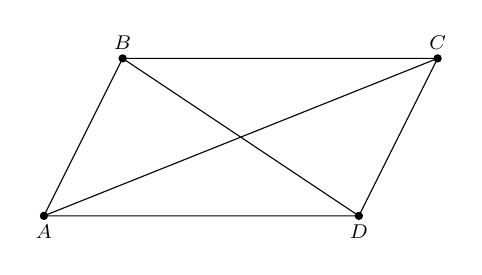
\begin{tikzpicture}[scale=1, font=\footnotesize, line join=round, line cap=round, >=stealth]
			\coordinate[label=below:$A$] (A) at (0,0);
			\coordinate[label=above:$B$] (B) at (1,2);
			\coordinate[label=above:$C$] (C) at (5,2);
			\coordinate[label=below:$D$] (D) at (4,0);	
			\draw (A)--(B)--(C)--(D)--(A)--(C) (D)--(B);
			\foreach \diem in {A,B,C,D}\fill (\diem)circle(1.5pt);
		\end{tikzpicture}
		}
		Mà $ABCD$ là hình bình hành nên ta có $BC=AD$ $\widehat{A}+\widehat{B}=180^\circ$ suy ra $\cos B =-\cos A$, do đó
	$$AC^2=AB^2+AD^2+2AB\cdot AD \cos A.$$
	Vậy $AC^2+BD^2=2AB^2+2AD^2$.
	}
\end{bt}

% từ: cau-hoi/lop10/0H4_He_thuc_luong_trong_tam_giac/0H4-3-1_Giai_tam_giac.tex
\begin{bt}%[0H4H3-1]%[ma:5359b064]
	Cho tam giác $ABC$,  biết $AB=3$; $AC=4$; $\widehat{A}=150^{\circ}$. Tìm diện tích của tam giác $ABC$
	 \loigiai{
		Với $AB=c$;  $AC=b$; $BC=a$.\\
		Ta có $S_{ABC}=\dfrac{1}{2} bc\sin A=\dfrac{1}{2} 3\cdot 4\cdot  \sin 150^{\circ}=3$.
	} 
\end{bt}

% từ: cau-hoi/lop10/0H9_Phuong_phap_toa_do_trong_mat_phang/0H9-2-3_Dang_thuc_ve_tich_vo_huong_hoac_do_dai.tex
\begin{bt}%[0H9H2-3]%[ma:a6f47c4a]
	Cho tam giác $ABC$. Tính diện tích tam giác $ABC$, với  $A(-2; 14)$, $B(4; -2)$, $C(5; -4)$.
	\loigiai{
		Ta có $\overrightarrow{BC}=(1;-2)\Rightarrow BC=\sqrt{5}$. Phương trình đường thẳng $BC$ đi qua $B$ có dạng $2(x-4)+1(y+2)=0\Leftrightarrow 2x+y-6=0$.\\
		Đường cao $AH$ của tam giác $ABC$: $AH=\dfrac{|2(-2)+14-6|}{\sqrt{5}}=\dfrac{4\sqrt{5}}{5}$.\\
		Do đó $S_{ABC}=\dfrac{1}{2}\cdot AH\cdot BC=\dfrac{4\sqrt{5}\cdot \sqrt{5}}{10}=2$(đvdt).
	}
\end{bt}

% từ: cau-hoi/lop10/0H9_Phuong_phap_toa_do_trong_mat_phang/0H9-3-1_Diem_vecto_he_so_goc_cua_duong_thang.tex
\begin{ex}%[0H9Y3-1]%[ma:7000214a]
	Cho đường tròn $(C)$ có phương trình  $(x+3)^2 + (y-4)^2 =2$. Tìm tâm và bán kính của đường tròn $(C)$.
	\choice 
		 {\True $I(-3; 4), R=\sqrt{2}$}
		 {$I(-3; -4), R=2$}
		 {$I(3; -4), R=\sqrt{2}$}
		{$I(3; -4),  R=2$}
	\loigiai{ 
		Từ  phương trình đường tròn $(C)$, ta suy ra đường tròn $(C)$ có tâm $I(-3;4)$ và bán kính $R=\sqrt{2}$.
	} 
\end{ex}

% từ: cau-hoi/lop10/0H9_Phuong_phap_toa_do_trong_mat_phang/0H9-4-1_Tim_tam_ban_kinh_va_dieu_kien_la_duong_tron.tex
\begin{bt}%[0H9B4-1]%[ma:f760cccc]
	Trong mặt phẳng tọa độ $ Oxy $, cho elip có phương  trình $ \dfrac{x^2}{169}+\dfrac{y^2}{25} =1$. Tìm tọa độ các tiêu điểm, độ dài trục lớn và độ dài trục nhỏ của elip.
	 \loigiai{
		Ta  có $ \dfrac{x^2}{169}+\dfrac{y^2}{25} =1 \Rightarrow a=13, b=5 \Rightarrow c=\sqrt{169 -25}=12$.\\
		Suy ra $ (E) $ có các tiêu điểm $ F_1(-12;0) $ và $ F_2(12;0)  $.\\
		Độ dài  trục lớn $ 2a=26 $ và độ dài trục nhỏ $ 2b=10 $.
	 }
\end{bt}

% từ: cau-hoi/lop10/0H9_Phuong_phap_toa_do_trong_mat_phang/0H9-4-1_Tim_tam_ban_kinh_va_dieu_kien_la_duong_tron.tex
\begin{bt}%[0H9B4-1]%[ma:74f37e2c]
	Trong mặt phẳng tọa  độ $Oxy$, cho Elip $(E)$ có phương trình $\dfrac{x^2}{9}+16y^2=1$. Tìm độ dài trục lớn, trục bé và các tiêu điểm của Elip.
	 \loigiai{
	\immini 
		 {
		Chuyển Elip  $(E)$ về dạng phương trình chính tắc
		$$\dfrac{x^2}{9}+16y^2=1\Leftrightarrow \dfrac{x^2}{9}+\dfrac{y^2}{\tfrac{1}{16}}=1.$$ 
		 }
		{ 
		\begin{tikzpicture}[scale=1.25,font=\footnotesize,line join=round,line cap=round,>=stealth]
				\draw (0,0) ellipse (3cm and  0.35cm);
				\draw[->] (-4,0) -- (4,0) node[below] {$x$}; 
				\draw[->]  (0,-1) -- (0,1) node[right] {$y$};
				\fill (0,0) circle  (1pt) node[below left]{$O$};
				\fill (2.8,0)  circle (1pt) node[below right]{$F_2$};
				\fill (-2.8,0) circle (1pt) node[below left]{$F_1$}; 
			\end{tikzpicture}
		 }\noindent
		Ta được  $a=3$, $b=\dfrac{1}{4}$ và $c=\sqrt{a^2-b^2}=\dfrac{\sqrt{143}}{4}$.\\
		 Khi đó
		\begin{itemize}
			\item Độ dài trục lớn là  $2a=6$.
			\item Độ dài trục bé  là $2b=\dfrac{1}{2}$.
			\item Các  tiêu điểm là $F_1\left( -\dfrac{\sqrt{143}}{4};0\right) $ và $F_2\left( \dfrac{\sqrt{143}}{4};0\right) $.
		\end{itemize}
	 }
\end{bt}

% từ: cau-hoi/lop11/1D1_Ham_so_luong_giac_va_phuong_trinh_luong/1D1-1-2_Chuyen_doi_don_vi_do_va_radian.tex
\begin{ex}%[1D1N1-2]%[ma:2d1c8986]
	Cho góc $\alpha \in  \left(\dfrac{\pi}{2};\pi\right)$. Chọn khẳng định đúng.
	\choice 
		 {\True $\cos \alpha <0 $}
		{$\sin \alpha <0 $} 
		{$\tan \alpha  >0 $}
		{$\cot \alpha >0  $}
	\loigiai{Giả sử điểm $M$ biểu diễn góc $\alpha \in  \left(\dfrac{\pi}{2};\pi\right)$.\\ Khi đó điểm $M$ thuộc cung phần tư thứ hai.\\
		Suy ra $\sin \alpha=y_M>0$; $\cos \alpha=x_M<0$; $\tan  \alpha=\dfrac{y_M}{x_M}<0 $; $\cot \alpha=\dfrac{x_M}{y_M}<0$.
	} 
\end{ex}

% từ: cau-hoi/lop11/1D1_Ham_so_luong_giac_va_phuong_trinh_luong/1D1-1-3_So_do_cua_mot_goc_luong_giac.tex
\begin{ex}%[1D1N1-3]%[ma:c5ae3913]
	Giá trị của biểu  thức $S=3-\sin ^{2} 90^\circ +2\cos ^{2} 60^\circ -3\tan ^{2} 45^\circ $ bằng
	 \choice
		 {$\dfrac{1}{2} $}
		{\True $-\dfrac{1}{2} $} 
		 {$1$}
		 {$3$}
	\loigiai{ 
	Ta có $S=3-\sin ^{2} 90^\circ +2\cos ^{2} 60^\circ  -3\tan ^{2} 45^\circ $$=3-1^2 +2\cdot\left(\dfrac{1}{2} \right)^{2} -3\cdot 1^2 $$=-\dfrac{1}{2} $.}
\end{ex}

% từ: cau-hoi/lop11/1D1_Ham_so_luong_giac_va_phuong_trinh_luong/1D1-1-3_So_do_cua_mot_goc_luong_giac.tex
\begin{ex}[c]%[1D1B1-3]%[ma:0811953c]
	 Cho hàm số $y=\dfrac{\sin2x}{2\cos x-3}$. Phát biểu nào sau đây là đúng?
	 \choice
		{Hàm số  đã cho là hàm số chẵn}
		{\True  Hàm số đã cho là hàm số lẻ}
		{Hàm số đã cho có  tập xác định $\mathscr{D}=\mathbb{R}\setminus\left\{\dfrac{3}{2}\right\}$}
		{Hàm số đã cho là hàm số không chẵn, không lẻ} 
	\loigiai{ 
		Ta  có $2\cos x-3\ne 0,\forall x\in\mathbb{R}$ nên tập xác định của hàm số là $\mathscr{D}=\mathbb{R}$.\\
		Ta có $y(-x)=\dfrac{\sin(-2x)}{2\cos(-x)-3}=\dfrac{-\sin2x}{2\cos x-3}=-y(x)$ nên hàm số đã cho là hàm số lẻ. 
	} 
\end{ex}

% từ: cau-hoi/lop11/1D1_Ham_so_luong_giac_va_phuong_trinh_luong/1D1-1-3_So_do_cua_mot_goc_luong_giac.tex
\begin{ex}[c]%[1D1B1-3]%[ma:b494495c]
	Trong các hàm số sau, hàm số nào là hàm  số lẻ?
	\choice 
		 {\True $y=\dfrac{x-\sin x}{\cos 2x}$}
		{$y=\dfrac{3x^2-\sin x}{\cos  3x}$}
		{$y=\dfrac{x-\sin  x}{\sin x}$}
		{$y=\dfrac{x^3-\sin x}{\sin  3x}$}
	 \loigiai{
	Xét  hàm số $y=f\left(x\right)=\dfrac{x-\sin x}{\cos 2x}$.\\
	 Tập xác định $\mathscr{D}=\mathbb{R}\setminus \left\{\dfrac{\pi}{4}+\dfrac{k\pi}{2}\mid dle| k\in \mathbb{Z}\right\}$.
	\begin{itemize}
		\item Với mọi $x\in \mathscr{D}$ thì $-x\in  \mathscr{D}$.
		\item $f\left(-x\right)=\dfrac{-x-\sin \left(-x\right)}{\cos  \left(-2x\right)}=\dfrac{-x+\sin x}{\cos 2x}=-\dfrac{x-\sin x}{\cos 2x}=-f\left(x\right)$.
	\end{itemize}
	Vậy $y=f\left(x\right)=\dfrac{x-\sin  x}{\cos 2x}$ là hàm số lẻ.
	 }
\end{ex}

% từ: cau-hoi/lop11/1D1_Ham_so_luong_giac_va_phuong_trinh_luong/1D1-1-4_Do_dai_cua_mot_cung_tron.tex
\begin{ex}%[1D1N1-4]%[ma:03f319ac]
	Cho góc $\alpha $ thoả mãn $90^\circ <\alpha <180^\circ $.  Trong các khẳng định sau, khẳng định nào đúng?
	\choice 
		{$\sin \alpha <0$} 
		{$\cos\alpha \ge  0$}
		{\True $\tan \alpha <0$} 
		{$\cot\alpha  >0$}
	 \loigiai{
	 Khẳng định đúng là $\tan \alpha <0$.}
\end{ex}

% từ: cau-hoi/lop11/1D1_Ham_so_luong_giac_va_phuong_trinh_luong/1D1-1-4_Do_dai_cua_mot_cung_tron.tex
\begin{ex}%[1D1H1-4]%[ma:7e4bb220]
	Cho $2\pi <\alpha <\dfrac{5\pi}{2}$. Kết quả đúng  là
	 \choice
		{\True $\tan \alpha >0$, $\cot \alpha  >0$}
		 {$\tan \alpha <0$, $\cot \alpha <0$}
		{$\tan \alpha >0$, $\cot \alpha <0$} 
		{$\tan  \alpha <0$, $\cot \alpha >0$}
	 \loigiai{
	Vì $2\pi <\alpha <\dfrac{5\pi}{2}$  nên $\tan \alpha >0;\cot \alpha >0$.}
\end{ex}

% từ: cau-hoi/lop11/1D1_Ham_so_luong_giac_va_phuong_trinh_luong/1D1-1-5_Duong_tron_luong_giac_va_ung_dung.tex
\begin{bt}%[1D1K1-5]%[ma:6660e688]
	Tìm giá trị lớn  nhất và giá trị nhỏ nhất của hàm số $y=4 \sin ^{2} x-4 \sin x+3$.
	 \loigiai{
		Tập xác định  $\mathscr{D}=\mathbb{R}$.\\
		Biến đổi $y=4  \sin ^{2} x-4 \sin x+3=\left(2\sin x+1\right)^2+2$.\\
		Với mọi  $x\in \mathbb{R}$ ta có
		\allowdisplaybreaks 
		\begin{eqnarray*}
			& & -1\leq \sin x\leq 1\\ 
			 &\Leftrightarrow& -1\leq 2\sin x+1\leq 3\\
			&\Leftrightarrow&0\leq \left(  2\sin x+1\right)^2\leq 9\\
			&\Leftrightarrow&2\leq \left( 2\sin x+1\right)^2+2\leq  11.
		\end{eqnarray*}
		Vậy $\max\limits_{x \in  \mathbb{R}} y=11$ khi $x=\dfrac{\pi}{2}$ và $\min\limits_{x \in \mathbb{R}} y=2$ khi $\sin x=-\dfrac{1}{2}$.
	 }
\end{bt}

% từ: cau-hoi/lop11/1D1_Ham_so_luong_giac_va_phuong_trinh_luong/1D1-1-5_Duong_tron_luong_giac_va_ung_dung.tex
\begin{ex}%[1D1K1-5]%[ma:ff973488]
	Tìm  giá trị lớn nhất và giá trị nhỏ nhất của hàm số $y=4 \sin ^{2} x-4 \sin x+3$.
	\loigiai{ 
		 Tập xác định $\mathscr{D}=\mathbb{R}$.\\
		Biến đổi $y=4 \sin ^{2}  x-4 \sin x+3=\left(2\sin x+1\right)^2+2$.\\
		Với mọi  $x\in \mathbb{R}$ ta có
		 \allowdisplaybreaks
		\begin{eqnarray*}
			&  & -1\leq \sin x\leq 1\\
			&\Leftrightarrow& -1\leq 2\sin x+1\leq 3\\ 
			&\Leftrightarrow&0\leq \left( 2\sin  x+1\right)^2\leq 9\\
			&\Leftrightarrow&2\leq \left( 2\sin  x+1\right)^2+2\leq 11.
		\end{eqnarray*}
		Vậy $\max\limits_{x \in \mathbb{R}} y=11$ khi $x=\dfrac{\pi}{2}$ và $\min\limits_{x  \in \mathbb{R}} y=2$ khi $\sin x=-\dfrac{1}{2}$.
	 }
\end{ex}

% từ: cau-hoi/lop11/1D1_Ham_so_luong_giac_va_phuong_trinh_luong/1D1-2-1_Cau_hoi_ly_thuyet.tex
\begin{ex}%[1D1H2-1]%[ma:a7547405]
	Phương trình $ \tan x=\tan\left(\dfrac{-\pi}{3}\right)$ có tất cả các  nghiệm là
	\choice 
		{\True  $x=\dfrac{-\pi}{3}+k\pi$, $(k\in\mathbb{Z})$}
		 {$x=\pm \dfrac{\pi}{3}+k\pi$, $(k\in\mathbb{Z})$}
		 {$x=\dfrac{-\pi}{3}+k2\pi$, $(k\in\mathbb{Z})$}
		{$x=\dfrac{\pi}{3}+k2\pi$, $(k\in\mathbb{Z})$} 
	 \loigiai{
		$\tan  x=\tan\left(\dfrac{-\pi}{3}\right) \Leftrightarrow x=\dfrac{-\pi}{3}+k\pi$, $(k\in\mathbb{Z})$.
	 }
\end{ex}

% từ: cau-hoi/lop11/1D1_Ham_so_luong_giac_va_phuong_trinh_luong/1D1-2-1_Cau_hoi_ly_thuyet.tex
\begin{ex}%[1D1B2-1]%[ma:5fa200b3]
	Phương  trình: $\sin x =\cos 5x$ có các nghiệm là
	 \choice
		{$x=\dfrac{\pi}{4}+k2\pi$ và $x=\dfrac{-\pi}{4}+k2\pi  , (k \in \mathbb{Z})$}
		{$x=\dfrac{-\pi}{12}+k\dfrac{\pi}{3}$ và  $x=\dfrac{\pi}{8}+k\dfrac{\pi}{2} , (k \in \mathbb{Z})$}
		{$x=\dfrac{\pi}{4}+k\pi$  và $x=\dfrac{-\pi}{4}+k\pi , (k \in \mathbb{Z})$}
		 {\True $x=\dfrac{\pi}{12}+k\dfrac{\pi}{3}$ và $x=\dfrac{-\pi}{8}+k\dfrac{\pi}{2} , (k \in \mathbb{Z})$}
	\loigiai{ 
		Ta có 
		\begin{eqnarray*}
			 & & \sin x =\cos 5x \\
			&\Leftrightarrow & \sin x = \sin \left(\dfrac{\pi}{2}-5x\right)\\ 
			&\Leftrightarrow & \hoac{& x=\dfrac{\pi}{2}-5x+k2\pi\\  &x = \dfrac{\pi}{2} + 5x + k2\pi}\\
			&\Leftrightarrow & \hoac{&  x=\dfrac{\pi}{12}+k\dfrac{\pi}{3}\\ &x=\dfrac{-\pi}{8}+k\dfrac{\pi}{2}}(k \in \mathbb{Z}).
		\end{eqnarray*}
	} 
\end{ex}

% từ: cau-hoi/lop11/1D1_Ham_so_luong_giac_va_phuong_trinh_luong/1D1-2-1_Cau_hoi_ly_thuyet.tex
\begin{ex}%[1D1B2-1]%[ma:c116e432]
	Cho phương trình $\sin{x}-\sin{2x}+\sin{3x}=0$. Nghiệm  của phương trình là
	\choice 
		{$x=\dfrac{\pi}{2}+k2\pi; x=k\pi, k\in \mathbb{Z}$} 
		 {$x=k\dfrac{\pi}{2}+k\pi, k\in \mathbb{Z}$}
		{\True $x=\pm \dfrac{\pi}{3}+k2\pi;  x=k\dfrac{\pi}{2}, k\in \mathbb{Z}$}
		{$x=\pm  \dfrac{\pi}{6}+k\pi, k\in \mathbb{Z}$}
	\loigiai{ 
		Phương trình $\sin{x}-\sin{2x}+\sin{3x}=0$ tương đương  với
		\begin{eqnarray*}
			2\sin{2x}\cos{x}-\sin{2x}=0 &\Leftrightarrow&  \sin{2x}(2\cos{x}-1)=0\\
			&\Leftrightarrow& \hoac{&\sin{2x}=0\\&\cos{x}=\dfrac{1}{2}} \;\Leftrightarrow\; \hoac{&x=\dfrac{k\pi}{2}\\&x=\pm\dfrac{\pi}{3}+k2\pi}  \,(k\in \mathbb{Z}).
		\end{eqnarray*}
	} 
\end{ex}

% từ: cau-hoi/lop11/1D1_Ham_so_luong_giac_va_phuong_trinh_luong/1D1-2-1_Cau_hoi_ly_thuyet.tex
\begin{ex}%[1D1B2-1]%[ma:3e2e97eb]
	Cho hai phương trình $\cos 3x-1=0$ (1); $\cos  2x=-\dfrac{1}{2}$ (2). Tập các nghiệm của phương trình (1) đồng thời là nghiệm của phương trình (2) là
	 \choice
		{\True $x=\pm \dfrac{2\pi}{3}+k2\pi $,  $k\in \mathbb{Z}$}
		{$x=k2\pi $,  $k\in \mathbb{Z}$}
		{$x=\dfrac{\pi}{3}+k2\pi  $, $k\in \mathbb{Z}$}
		{$x=\pm \dfrac{\pi}{3}+k2\pi $, $k\in  \mathbb{Z}$}
	 \loigiai{
		 Ta có $\cos 3x-1=0 \Leftrightarrow \cos 3x=1 \Leftrightarrow x=k\dfrac{2\pi}{3}$, $k\in \mathbb{Z}$. \\
		$\cos 2x=-\dfrac{1}{2} \Leftrightarrow 2x=\pm \dfrac{2\pi}{3}+k2\pi \Leftrightarrow x=\pm \dfrac{\pi}{3}+k\pi $,  $k\in \mathbb{Z}$. \\
	Biểu  diễn các nghiệm trên đường tròn lượng giác ta có tập các nghiệm của phương trình (1) đồng thời là nghiệm của phương trình (2) là $x=\pm \dfrac{2\pi}{3}+k2\pi $, $k\in \mathbb{Z}$.}
\end{ex}

% từ: cau-hoi/lop11/1D1_Ham_so_luong_giac_va_phuong_trinh_luong/1D1-2-1_Cau_hoi_ly_thuyet.tex
\begin{ex}%[1D1Y2-1]%[ma:f7378a8a]
	Tập nghiệm của phương  trình $\tan \left(x-\dfrac{\pi }{6}\right)=\sqrt{3}$ là
	 \choice
		{  $S=\left\{\dfrac{-\pi }{6}+k\pi,k\in \mathbb{Z}\right\}$}
		{ $S=\left\{\dfrac{\pi }{3}+k\pi,k\in  \mathbb{Z}\right\}$}
		{\True $S=\left\{\dfrac{\pi }{2}+k\pi,k\in \mathbb{Z}\right\}$} 
		{ $S=\left\{\dfrac{\pi }{2}+k2\pi,k\in  \mathbb{Z}\right\}$}
	 \loigiai{
		Ta có $\tan \left(x-\dfrac{\pi  }{6}\right)=\sqrt{3}\Leftrightarrow x-\dfrac{\pi }{6}=\dfrac{\pi }{3}+k\pi \Leftrightarrow x=\dfrac{\pi }{2}+k\pi $, $ k\in \mathbb{Z}$.
	 }
\end{ex}

% từ: cau-hoi/lop11/1D1_Ham_so_luong_giac_va_phuong_trinh_luong/1D1-2-1_Cau_hoi_ly_thuyet.tex
\begin{ex}%[1D1Y2-1]%[ma:0182d924]
	Tập nghiệm $S$ của phương  trình $3\tan x-\sqrt{3}=0$ là
	\choice 
		{$S=\left\{\dfrac{\pi}{6}+k2\pi,k\in  \mathbb{Z}\right\}$}
		 {$S=\left\{\dfrac{\pi}{6}+\dfrac{k\pi}{3},k\in \mathbb{Z}\right\}$}
		{\True $S=\left\{\dfrac{\pi}{6}+k\pi,k\in  \mathbb{Z}\right\}$}
		{$S=\left\{\dfrac{\pi}{6}+\dfrac{k2\pi}{3},k\in \mathbb{Z}\right\}$} 
	\loigiai{ 
		Ta có $3\tan x-\sqrt{3}=0\Leftrightarrow \tan  x=\dfrac{\sqrt{3}}{3}\Leftrightarrow x=\dfrac{\pi}{6}+k\pi,k\in \mathbb{Z}.$ \\
	 Vậy tập nghiệm của phương trình là $S=\left\{\dfrac{\pi}{6}+k\pi,k\in \mathbb{Z}\right\}.$}
\end{ex}

% từ: cau-hoi/lop11/1D1_Ham_so_luong_giac_va_phuong_trinh_luong/1D1-5-3_Phuong_trinh_co_ban_dung_Radian.tex
\begin{ex}%[1D1H5-3]%[ma:bec67f4e]
 Một nhà thực vật học đo chiều dài trung bình của $74$ lá cây (đơn  vị: milimét) và thu được bảng tần số ghép nhóm như sau
 {\fontsize{10pt}{12pt}\selectfont 
 \begin{center}
  \begin{tabular}{|c|c|c|c|c|c|c|c|}
   \hline 
   Nhóm & $[5{,}45; 5{,}85)$ & $[5{,}85; 6{,}25)$ & $[6{,}25; 6{,}65)$ & $[6{,}65; 7{,}05)$  & $[7{,}05; 7{,}45)$ & $[7{,}45; 7{,}85)$ & $[7{,}85; 8{,}25)$ \\ \hline
   Giá trị đại diện & 5,65 & 6,05 & 6,45 & 6,85 & 7,25 & 7,65 & 8,05  \\ \hline
   Tần số & 5 &  9 & 15 & 15 & 19 & 8 & 2 \\ \hline
  \end{tabular}
 \end{center}}
  \choiceTF
  {Chiều dài trung bình của $74$ lá cây bằng $\approx 6{,}4$ (mm)} 
  {\True Độ  dài nhóm là $0{,}4$}
  {Nhóm chứa mốt  là $[7{,}05;7{,}45)$}
  {Mốt  của mẫu số liệu ghép nhóm là $\approx 6{,}65$}
  \loigiai{
  \begin{itemchoice}
   \itemch \textbf{Sai}. Chiều dài trung bình  của 74 lá cây là:
   $$\begin{aligned}
   \bar{x} &  =\dfrac{5,65.5+6,05.9+6,45 \cdot 15+6,85 \cdot 19+7,25.16+7,65 \cdot 8+8,05.2}{74} \\
   & =\dfrac{5029}{740} \approx 6{,}8({~mm})  .
  \end{aligned}
  $$ 
   \itemch \textbf{Đúng}. Độ dài nhóm là $0{,}4$.
   \itemch \textbf{Sai}.Nhóm chứa mốt là ${[6,65; 7,05)}$,\\
   trong đó
  ${u_m=6{,}65;  u_{m+1}=7{,}05; u_{m+1}-u_m=0{,}4; n_m=19; n_{m-1}=15; n_{m+1}=16
  }$. 
  \itemch \textbf{Sai}. Mốt của  mẫu số liệu ghép nhóm là:
  ${M_0=6{,}65+\dfrac{19-15}{(19-15)+(19-16)} \cdot 0{,}4  \approx 6{,}88.}$
 \end{itemchoice}
} 
\end{ex}

% từ: cau-hoi/lop11/1D1_Ham_so_luong_giac_va_phuong_trinh_luong/1D1-5-3_Phuong_trinh_co_ban_dung_Radian.tex
\begin{ex}%[1D1H5-3]%[ma:5897de2e]
 Người ta tiến hành phỏng vấn 30 người về một bộ phim mới chiếu trên truyền hình. Người điều tra yêu cầu cho điểm bộ phim (thang điểm là 100). Kết quả được trình bày trong bảng phân bố tần số ghép lớp sau đây 
 \begin{center}
  \begin{tabular}{|c|c|c|c|c|c|}
   \hline 
   Số điểm & $[50;60)$ & $[60; 70)$ &  $[70;80)$ & $[80;90)$ & $[90;100)$ \\ \hline
   Số người & 2  & 6 & 10 & 8 & 4 \\ \hline
  \end{tabular}
 \end{center}
 \choiceTF 
  {\True Ước lượng số trung  bình của mẫu ghép là $77$}
  {\True Giá trị đại diện  của nhóm ${[90; 100)}$ là $95$}
  {Nhóm chứa mốt của mẫu số liệu  trên là nhóm $[80;90)$}
  {Mốt của mẫu số liệu là  $74{,}67$}
 \loigiai{ 
  \begin{itemchoice}
    \itemch \textbf{Đúng}.
   \begin{center}
    \begin{tabular}{|c|c|c|c|c|c|}
     \hline 
      Số điểm & $[50;60)$ & $[60; 70)$ & $[70;80)$ & $[80;90)$ & $[90;100)$ \\ \hline
     Giá trị đại diện & $55$ & $65$ & $75$ & $85$ &  $95$ \\ \hline
     Số người & 2 & 6 & 10 & 8 & 4 \\ \hline 
    \end{tabular}
   \end{center}
   Ước lượng số trung bình của mẫu ghép  là:
   $$\bar{x}=\dfrac{55\cdot2+65\cdot6+75\cdot10+85\cdot8+95\cdot4}{30}=77.$$ 
   \itemch \textbf{Đúng}.Giá trị đại diện của  nhóm ${[90; 100)}$ là $95$.
   \itemch \textbf{Sai}. Nhóm chứa mốt của mẫu số liệu trên  là nhóm $[70; 80)$.
    \itemch \textbf{Sai}.
    Do đó, $u_m=70; n_{m-1}=6; n_m=10; n_{m+1}=8; u_{m+1}-u_m=80-70=10$.\\
   $M_{\circ}=70+\dfrac{10-6}{(10-6)+(10-8)} \cdot  10=76{,}67.$
  \end{itemchoice}
  }
\end{ex}

% từ: cau-hoi/lop11/1D1_Ham_so_luong_giac_va_phuong_trinh_luong/1D1-5-3_Phuong_trinh_co_ban_dung_Radian.tex
\begin{ex}%[1D1H5-3]%[ma:a43c4d1c]
 Số cuộc điện thoại một người thực hiện  mỗi ngày trong 30 ngày được lựa chọn ngẫu nhiên được thống kê trong bảng sau:
 \begin{center}
  \begin{tabular}{|c|c|c|c|c|c|}
    \hline
   Số cuộc gọi & $[2{,}5; 5{,}5)$ & $[5{,}5; 8{,}5)$ & $[8{,}5; 11{,}5)$ & $[11{,}5; 14{,}5)$ & $[14{,}5; 17{,}5)$ \\  \hline
   Số ngày & 5 & 13 &  7 & 3 & 2 \\ \hline
  \end{tabular}
 \end{center}
  \choiceTF
  {Số cuộc gọi trung bình  mỗi ngày là $8{,}1$}
   {\True Nhóm chứa mốt là $[5{,}5; 8{,}5)$}
  {\True  Mốt của mẫu số liệu ghép nhóm là $\approx 7{,}21$}
  {Người đó thực hiện  tối đa khoảng 8 cuộc gọi mỗi ngày}
  \loigiai{
  \begin{itemchoice}
   \itemch \textbf{Sai}. Ta viết lại bảng  tần số ghép nhóm theo giá trị đại diện là
   \begin{center}
    \begin{tabular}{|c|c|c|c|c|c|}
      \hline
     Số cuộc gọi & $[2{,}5; 5{,}5)$ & $[5{,}5;  8{,}5)$ & $[8{,}5; 11{,}5)$ & $[11{,}5; 14{,}5)$ & $[14{,}5; 17{,}5)$ \\ \hline
     Giá trị đại diện & 4 & 7 & 10 & 13 & 16 \\  \hline
     Số ngày & 5 & 13 &  7 & 3 & 2 \\ \hline
    \end{tabular}
   \end{center}
   Số cuộc gọi trung bình  mỗi ngày là:
   $$\bar{x}=\dfrac{4\cdot5+7\cdot13+10\cdot7+13\cdot3+16\cdot2}{30}=8{,}4.$$ 
   \itemch \textbf{Đúng}. Nhóm  chứa mốt là $[5{,}5; 8{,}5)$.
   \itemch \textbf{Đúng}. Ta có  ${u_m=5,5; u_{m+1}=8,5 \Rightarrow u_{m+1}-u_m=3; n_m=13; n_{m-1}=5; n_{m+1}=7}$.\\
   Vì vậy mốt của mẫu số liệu ghép nhóm  là
   $$M_0=5,5+\frac{13-5}{(13-5)+(13-7)} \cdot  3=\frac{101}{14} \approx 7{,}21.$$
   \itemch \textbf{Sai}. Vậy người đó thực hiện tối đa khoảng 7 cuộc  gọi mỗi ngày.
  \end{itemchoice}
 } 
\end{ex}

% từ: cau-hoi/lop11/1D1_Ham_so_luong_giac_va_phuong_trinh_luong/1D1-5-5_Phuong_trinh_dua_ve_dang_co_ban.tex
\begin{bt}%[1D1H5-5]%[ma:24cd9ccc]
% nguon: Archive/2024/SP-K10-K11-LyVanHoang_TVN-023/11. C1-LuongGiac-lvhoang_TVN-023/dataC1K11/Chuong1-Bai4-Dang5-Phuongtrinhduavecoban.tex #2031
%[Bài giảng 11, Trần Tony]
	Giải các phương trình sau
	\begin{listEX}[2]
		\item $6\cos^2 x+5\sin x-7=0$.
		\item $\cos 2x+\cos x+1=0$.
		\item $3\sin^2 2x+7\cos 2x-3=0$.
		\item $7\tan x-4\cot x=12$.
	\end{listEX}
	\loigiai{
		\begin{enumerate}[a)]
			\item Đặt $t=\sin x$, $-1\le t\le 1$, phương trình đã cho trở thành $6(1-t^2)+5t-7=0$, ta được $t=\dfrac{1}{2}$ hoặc $t=\dfrac{1}{3}$.\\
			Với $t=\dfrac{1}{2}$, ta có $\sin x=\dfrac{1}{2} \Leftrightarrow \hoac{&x=\dfrac{\pi}{6}+k2\pi\\ &x=\dfrac{5\pi}{6}+k2\pi}\ (k\in\mathbb{Z})$.\\
			Với $t=\dfrac{1}{3}$, ta có $\sin x=\dfrac{1}{3}=\sin\alpha\Leftrightarrow \hoac{&x=\alpha + k2\pi\\ & x=\pi-\alpha + k2\pi}\ (k\in\mathbb{Z})$.
			
			\item Đặt $t=\cos x$, $-1\le t\le 1$, phương trình đã cho trở thành $2t^2-1+t+1=0$, ta được $t=0$ hoặc $t=-\dfrac{1}{2}$.\\
			Với $t=0$, ta có $\cos x=0\Leftrightarrow x=k2\pi$ ($k\in\mathbb{Z}$).\\
			Với $t=-\dfrac{1}{2}$, ta có $\cos x=-\dfrac{1}{2}\Leftrightarrow x=\pm \dfrac{2\pi}{3}+k2\pi$ ($k\in\mathbb{Z}$).
			\item Đặt $t=\cos 2x$, $-1\le t\le 1$. Phương trình đã cho trở thành
			\begin{eqnarray*}
				&&3\left(1-t^2\right) +7t -3=0\\
				&\Leftrightarrow &3t^2-7t=0\\
				&\Leftrightarrow &\hoac{&t=0\\ &t=\dfrac{7}{3}\quad(\text{loại}).}
			\end{eqnarray*}
			Ta có $\cos 2x=0$ hay $x=\dfrac{\pi}{4}+\dfrac{k\pi}{2}\ (k\in\mathbb{Z})$.\\
			Vậy tập nghiệm của phương trình đã cho là $S=\left\{\dfrac{\pi}{4}+\dfrac{k\pi}{2}, k\in\mathbb{Z}\right\}$.
			
			\item Đặt $t=\tan x$, $t\ne 0$. Phương trình đã cho trở thành
			\begin{eqnarray*}
				&&7t-\dfrac{4}{t}=12\\
				&\Leftrightarrow &7t^2-12t-4=0\\
				&\Leftrightarrow &\hoac{&t=2\\ &t=-\dfrac{2}{7}.}
			\end{eqnarray*}
			Với $t=2$ ta có $\tan x=2=\tan\alpha\Leftrightarrow x=\alpha +k\pi,\ (k\in\mathbb{Z})$.\\
			Với $t=-\dfrac{2}{7}$ ta có $\tan x=-\dfrac{2}{7}=\tan\beta\Leftrightarrow x=\beta+k\pi\ (k\in\mathbb{Z})$.\\
			Vậy tập nghiệm của phương trình đã cho là $S=\left\{\alpha +k\pi,\beta+k\pi, k\in\mathbb{Z} \right\}$.
		\end{enumerate}
	}
\end{bt}

% từ: cau-hoi/lop11/1D1_Ham_so_luong_giac_va_phuong_trinh_luong/1D1-5-5_Phuong_trinh_dua_ve_dang_co_ban.tex
\begin{bt}%[1D1H5-5]%[ma:9f9fed8a]
% nguon: Archive/2024/SP-K10-K11-LyVanHoang_TVN-023/11. C1-LuongGiac-lvhoang_TVN-023/dataC1K11/Chuong1-Bai4-Dang5-Phuongtrinhduavecoban.tex #2033
%[Bài giảng 11, Trần Tony]
	Giải các phương trình sau
	\begin{listEX}[2]
		\item $\cos ^2x+\cos x-2=0$;
		\item $2\sin^2 x -5\sin x +2=0$;
		\item $3\tan^2 x-2\sqrt{3}\tan x+1=0$.
	\end{listEX}
	\loigiai{
		\begin{enumerate}[a)]
			\item Đặt $t=\cos x$, $-1\le t\le 1$. Phương trình trở thành $t^2+t-2$, ta được $t=1$ hoặc $t=-2$.\\Kết hợp điều kiện ta có $t=1$, do đó $\cos x=1$ hay $x=k2\pi\ (k\in\mathbb{Z})$.\\
			Vậy tập nghiệm của phương trình đã cho là $S=\left\{ k2\pi, k\in\mathbb{Z}  \right\}$.
			\item Đặt $t=\sin x$, $-1\le t\le 1$. Phương trình trở thành $2t^2-5t+2=0$, ta được $t=\dfrac{1}{2}$ hoặc $t=2$.\\Kết hợp điều kiện, ta có $t=\dfrac{1}{2}$, do đó $\sin x=\dfrac{1}{2}$ hay $x=\dfrac{\pi}{6}+k2\pi$ hoặc $x=\dfrac{5\pi}{6}+k2\pi$ ($k\in\mathbb{Z}$).\\
			Vậy tập nghiệm của phương trình đã cho là $S=\left\{\dfrac{\pi}{6}+k2\pi, \dfrac{5\pi}{6}+k2\pi, k\in\mathbb{Z}\right\}$.
			\item Đặt $t=\tan x$, phương trình đã cho trở thành $3t^2-2\sqrt{3}t+1=0$, ta được $t=\dfrac{1}{\sqrt{3}}$.\\Do đó $\tan x=\dfrac{1}{\sqrt{3}}$ hay $x=\dfrac{\pi}{6}+k\pi$ ($k\in\mathbb{Z}$).\\
			Vậy tập nghiệm của phương trình đã cho là $S=\left\{ \dfrac{\pi}{6}+k\pi, k\in\mathbb{Z}  \right\}$.
		\end{enumerate}
	}
\end{bt}

% từ: cau-hoi/lop11/1D1_Ham_so_luong_giac_va_phuong_trinh_luong/1D1-5-5_Phuong_trinh_dua_ve_dang_co_ban.tex
\begin{bt}%[1D1V5-5]%[ma:3633c8b6]
% nguon: Archive/SP_KhoLatex/ID6_old/11-OT-PTLuongGiacCoBan.tex #3097
%[ĐGNL-ĐGTD-2022, Tran Tony]
	Giải phương trình $\sin 4x \cos x =\sin5x \cos2x$.
	\loigiai{Phương trình đã cho tương đương với  $$ \dfrac{1}{2} \left(\sin5x + \sin3x\right) =  \dfrac{1}{2} \left(\sin7x + \sin3x\right) \Leftrightarrow \sin5x = \sin7x \Leftrightarrow \hoac{&x= k\pi\\& x=\dfrac{\pi}{12}+\dfrac{k\pi}{6}}\, (k\in \mathbb{Z}).$$
	}
\end{bt}

% từ: cau-hoi/lop11/1D1_Ham_so_luong_giac_va_phuong_trinh_luong/1D1-5-5_Phuong_trinh_dua_ve_dang_co_ban.tex
\begin{bt}%[1D1H5-5]%[ma:5d8ceb33]
% nguon: Archive/SP_KhoLatex/ID6_old/12-OT-PTLuongGiacThuongGap.tex #3703

	Giải phương trình $\sin 2x\cos x=\sin 7x\cos 4x$.
	\loigiai
	{
		Ta có
		\allowdisplaybreaks
		\begin{eqnarray*}
			&& \sin 2x\cos x=\sin 7x\cos 4x \\
			&\Leftrightarrow & \dfrac{1}{2}\left(\sin 3x + \sin x\right) = \dfrac{1}{2}\left(\sin 11x + \sin 3x\right)\\
			&\Leftrightarrow & \sin x = \sin 11x \\
			&\Leftrightarrow & \left[\begin{aligned}&11x=x+k2\pi	\\&11x=\pi-x+k2\pi\end{aligned}\right. , \left(k\in\mathbb{Z}\right)\\
			&\Leftrightarrow & \left[\begin{aligned}&x=\dfrac{k\pi}{5}	\\&x=\dfrac{\pi}{12}+\dfrac{k\pi}{6}\end{aligned}\right. , \left(k\in\mathbb{Z}\right).
		\end{eqnarray*}
		Vậy phương trình đã cho có các nghiệm $x=\dfrac{k\pi}{5}$, $x=\dfrac{\pi}{12}+\dfrac{k\pi}{6}$ với $k\in\mathbb{Z}$.
	}
\end{bt}

% từ: cau-hoi/lop11/1D1_Ham_so_luong_giac_va_phuong_trinh_luong/1D1-5-5_Phuong_trinh_dua_ve_dang_co_ban.tex
\begin{bt}%[1D1V5-5]%[ma:80613261]
% nguon: Archive/2024/TOAN_11_XE/TOAN_11_XE/data4/11C1/KNTT-1.OTC.tex #1117
%[Trần Công Duy]
	Giải các phương trình sau:
	\begin{listEX}[3]
		\item $\sin 2 x+\cos 3 x=0$
		\item $\sin x \cos x=\dfrac{\sqrt{2}}{4}$;
		\item $\sin x+\sin 2 x=0$.
	\end{listEX}
	\loigiai{
		\begin{listEX}
			\item $\sin 2 x+\cos 3x=0$
			\allowdisplaybreaks
			\begin{eqnarray*}
				\sin 2x+\cos 3x=0 &\Leftrightarrow& \cos 3x=-\sin 2x \\
				&\Leftrightarrow& \cos 3x=\sin \left(-2x\right)\\
				&\Leftrightarrow& \cos 3x=\cos \left(\dfrac{\pi}{2}+2x\right)\\
				&\Leftrightarrow&\hoac{&3x=\dfrac{\pi}{2}+2x+k2\pi\\&3x=-\dfrac{\pi}{2}-2x+k2\pi}\Leftrightarrow\hoac{&x=\dfrac{\pi}{2}+k2\pi\\&x=-\dfrac{\pi}{10}+\dfrac{k2\pi}{5}} (k\in\mathbb{Z}).
			\end{eqnarray*}	
			Vậy phương trình có các nghiệm là $x=\dfrac{\pi}{2}+k2\pi, k\in\mathbb{Z}$ và $x=-\dfrac{\pi}{10}+\dfrac{k2\pi}{5}, k\in\mathbb{Z}$.
			\item $\sin x \cos x=\dfrac{\sqrt{2}}{4}$;
			\allowdisplaybreaks
			\begin{eqnarray*}
				&&\sin x \cos x=\dfrac{\sqrt{2}}{4} \\
				&\Leftrightarrow& 2\sin x\cos x=\dfrac{\sqrt{2}}{2}\\
				&\Leftrightarrow&\sin 2x=\dfrac{\sqrt{2}}{2}=\sin \dfrac{\pi}{4} \\
				&\Leftrightarrow& \hoac{&2x=\dfrac{\pi}{4}+k2\pi\\&2x=\pi-\dfrac{\pi}{4}+k2\pi} 
				\Leftrightarrow\hoac{&x=\dfrac{\pi}{8}+k\pi\\&x=\dfrac{3\pi}{8}+k\pi} (k\in\mathbb{Z}).
			\end{eqnarray*}	
			Vậy phương trình có các nghiệm là $x=\dfrac{\pi}{8}+k\pi, k\in\mathbb{Z}$ và $x=\dfrac{3\pi}{8}+k\pi, k\in\mathbb{Z}$.
			\item $\sin x+\sin 2 x=0$.
			\allowdisplaybreaks
			\begin{eqnarray*}
				&&\sin x+\sin 2 x=0 \\
				&\Leftrightarrow& \sin x+2\sin x\cos x=0 \\
				&\Leftrightarrow& \sin x \left(1+2\cos x\right)=0 \\
				&\Leftrightarrow& \hoac{&\sin x=0\\&1+2\cos x=0} \\
				&\Leftrightarrow& \hoac{&\sin x=0\\&\cos x=-\dfrac{1}{2}}\Leftrightarrow \hoac{&x=k\pi\\&x=\pm \dfrac{2\pi}{3}+k2\pi} (k\in\mathbb{Z}).
			\end{eqnarray*}	
			Vậy phương trình có các nghiệm là $k\pi, k\in\mathbb{Z}$ và $x=\pm \dfrac{2\pi}{3}+k2\pi, k\in\mathbb{Z}$.
		\end{listEX}
	}
\end{bt}

% từ: cau-hoi/lop11/1D2_Day_so_Cap_so_cong_Cap_so_nhan/1D2-2-2_Nhan_dien_cap_so_cong_cong_sai.tex
\begin{ex}%[1D2H2-2]%[ma:f25a9321]
	Cho  dãy số $(u_n)$ với $u_n=1+2^n$. Khi đó số hạng $u_{2018}$ bằng
	 \choice
		{$2^{2018}$} 
		 {$2017+2^{2017}$}
		{\True$1+2^{2018}$} 
		 {$2018+2^{2018}$}
	\loigiai{Số hạng $u_{2018}$  là $u_{2018}=1+2^{2018}$.
	} 
\end{ex}

% từ: cau-hoi/lop11/1D2_Day_so_Cap_so_cong_Cap_so_nhan/1D2-2-3_So_hang_tong_quat_cua_cap_so_cong.tex
\begin{ex}%[1D2H2-3]%[ma:547cccc1]
	Cho dãy  số $(u_n)$ xác định bởi $\heva{& u_1 = 2\\& u_{n+1} = u_n + 5, n \in \mathbb{N}^*}$. Tính $u_{10}$.
	\choice 
		{$57$} 
		{$62$} 
		 {\True $47$}
		 {$52$}
	\loigiai{ 
		Từ $\heva{& u_1 = 2\\& u_{n+1} = u_n + 5,  n \in \mathbb{N}^*.}$\\
		 Ta có $u_{n+1} - u_n = 5$ nên dãy $(u_n)$ là một cấp số cộng với công sai $d = 5$.\\
		Nên $u_{10} = u_1 + 9\cdot d = 2 + 9 \cdot  5 = 47$.
	 }
\end{ex}

% từ: cau-hoi/lop11/1D2_Day_so_Cap_so_cong_Cap_so_nhan/1D2-3-3_So_hang_tong_quat_cua_cap_so_nhan.tex
\begin{ex}%[1D2H3-3]%[ma:5fc4a294]
	 Cho dãy số $\left(u_n\right)$ biết $\heva{&u_1=3\\&u_{n+1}=3u_n}, \forall n\in{N^*}$. Tìm số hạng tổng quát của dãy số $(u_n)$.
	 \choice
		{\True $u_n=3^n$} 
		 {$u_n=n^{n+1}$}
		 {$u_n=3^{n+1}$}
		 {$u_n=3^{n-1}$}
	 \loigiai{
		Ta có  $u_1=3$ và $\dfrac{u_{n+1}}{u_n}=3$\\
		Suy ra dãy số $\left(u_n\right)$ là cấp số nhân với  $\heva{&u_1=3\\ &q=3.}$\\
	Do đó $u_n=u_1 \cdot  q^{n-1}=3 \cdot 3^{n-1}=3^n$.}
\end{ex}

% từ: cau-hoi/lop11/1D2_Day_so_Cap_so_cong_Cap_so_nhan/1D2-3-8_Toan_thuc_te_ap_dung_cap_so_nhan.tex
\begin{ex}%[1D2V3-8]%[ma:51735299]
	\immini[thm]{Cho hình vuông $C_1$ có cạnh bằng $4$. Người ta chia mỗi cạnh của hình vuông thành bốn phần bằng nhau và nối các điểm chia một cách thích hợp để có hình vuông $C_2$ như  hình vẽ bên.
	Từ hình vuông $C_2$ lại làm tiếp như trên để nhận được hình vuông $C_3$,\ldots. Tiếp tục quá trình trên, ta nhận được dãy các hình vuông $C_1,\,C_2,\,C_3,\ldots,C_n,\ldots$. Gọi $a_n$ là độ dài của cạnh hình vuông $C_n$. Tính tổng diện tích của  các hình vuông (kết quả làm tròn đến hàng phần chục).}
	{ 
	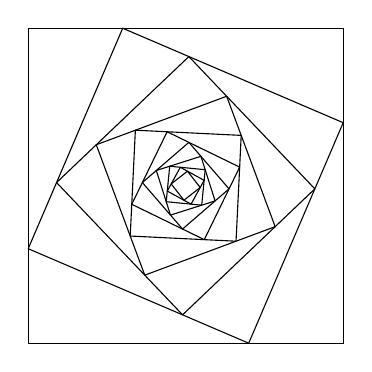
\begin{tikzpicture}[line cap=round,line join=round]
			 \def\a{2}
			\def\t{.7} 
			 \path
				 (-\a,-\a) coordinate (A1)
				(-\a,\a) coordinate  (B1)
				 (\a,\a) coordinate (C1)
				(\a,-\a) coordinate  (D1);
			\draw  (A1)--(B1)--(C1)--(D1)--cycle;
			\foreach  \i[count=\j from 2] in {1,...,10}
			 \draw
				 (barycentric cs:A\i=\t,B\i=1-\t) coordinate (A\j)--
				(barycentric  cs:B\i=\t,C\i=1-\t) coordinate (B\j)--
				(barycentric  cs:C\i=\t,D\i=1-\t) coordinate (C\j)--
				(barycentric cs:D\i=\t,A\i=1-\t)  coordinate (D\j)--cycle;
		\end{tikzpicture}
	 }
	\shortans{42,7} 
	 \loigiai{
		Gọi hình vuông $C_1$ có cạnh $a_1=4$ và có  diện tích là $S_1=a_1^2$.\\
		Cạnh của hình vuông $C_2$ là $a_2=\sqrt{{{\left(  \dfrac{3}{4}{a_1} \right)}^2}+{{\left( \dfrac{1}{4}{a_1} \right)}^2}}=\dfrac{a_1\sqrt{10}}{4}$.\\
		Diện  tích của hình vuông $C_2$ là $S_2=\dfrac{5}{8}{a_1}^2=\dfrac{5}{8}{S_1}$.\\
		Cạnh của hình vuông $C_3$ là $a_3=\sqrt{{{\left( \dfrac{3}{4}{a_2}  \right)}^2}+{{\left( \dfrac{1}{4}{a_2} \right)}^2}}=\dfrac{a_2\sqrt{10}}{4}=a_1.{{\left( \dfrac{\sqrt{10}}{4} \right)}^2}$.\\
		Diện tích của  hình vuông $C_3$ là $S_3={{\left( \dfrac{5}{8} \right)}^2}{a_1}^2={{\left( \dfrac{5}{8} \right)}^2}{S_1}$.\\
		Lý luận tương tự ta có dãy các hình vuông $C_1,\,C_2,\,C_3,\ldots,C_n,\ldots$ có các diện tích lần lượt là $S_1,\,S_2,\,S_3,\ldots,S_n,\ldots$ tạo thành một cấp số nhân lùi vô hạn với số hạng đầu  là: $u_1=S_1=16$ và công bội $q=\dfrac{5}{8}$.\\
		Vậy tổng diện tích của các hình  vuông là\\
	$S=S_1+\,S_2+\,S_3+\ldots+S_n+\ldots=\dfrac{u_1}{1-q}=\dfrac{16}{1-\tfrac{5}{8}}=\dfrac{128}{3}\approx  42{,}7$.}
\end{ex}

% từ: cau-hoi/lop11/1D3_Gioi_han_Ham_so_lien_tuc/1D3-1-1_Cau_hoi_ly_thuyet.tex
\begin{ex}%[1D3N1-1]%[ma:de7fb660]
	Trong các khẳng định dưới đây, khẳng định nào \textbf{sai}? 
	 \choice
		 {\True $\lim\limits_{n \to +\infty} q^n=0$}
		{$\lim\limits_{n \to +\infty} \dfrac{1}{n^k}=0$ với $k$  nguyên dương}
		 {$\lim\limits_{n \to +\infty} \dfrac{1}{n}=0$}
		{Nếu $u_n=c$ ($c$ là hằng số) thì $\lim\limits_{n \to +\infty} u_n=\lim c=c$} 
	\loigiai{ 
	Ta có $\lim\limits_{n \to +\infty} q^n=0$ khi  $|q|<1$; $\lim\limits_{n \to +\infty} q^n=+\infty$ khi $q>1$.}
\end{ex}

% từ: cau-hoi/lop11/1D3_Gioi_han_Ham_so_lien_tuc/1D3-1-2_Phuong_phap_dat_thua_so_chung_lim_huu_han.tex
\begin{ex}%[1D3N1-2]%[ma:dbfff29d]
	Tìm giới hạn sau  $\lim\limits_{n \to +\infty} \dfrac{4n -1}{-n -1}$.
	 \choice
		 {\True $-4$}
		{$7$} 
		{$-7$} 
		 {$4$}
	\loigiai{ 
		Chia cả tử và mẫu  cho $n$ ta được
		$$\lim\limits_{n \to +\infty} \dfrac{4n  -1}{-n -1} = -4.$$
		Vậy $\lim\limits_{n  \to +\infty} \dfrac{4n -1}{-n -1} = -4$.
	 }
\end{ex}

% từ: cau-hoi/lop11/1D3_Gioi_han_Ham_so_lien_tuc/1D3-1-2_Phuong_phap_dat_thua_so_chung_lim_huu_han.tex
\begin{ex}%[1D3N1-2]%[ma:bd2ff02c]
 Mỗi kết quả giới  hạn dưới đây đúng hay sai?
  \choiceTF
  {$\lim\limits_{n  \to +\infty} \dfrac{2n+3}{2n-1}=2$}
  {\True $\lim\limits_{n  \to +\infty} \dfrac{2n^2+3}{n^2+1}=2$}
  {$\lim\limits_{n \to +\infty} \dfrac{2n^2+n+3}{3-n^2}=\dfrac{2}{3}$} 
  {\True  $\lim\limits_{n \to +\infty} \dfrac{2n+3}{n^2+2}=0$}
 \loigiai{ 
  \begin{itemchoice}
   \itemch $\lim\limits_{n \to +\infty} \dfrac{2n+3}{2n-1}=\lim\limits_{n \to +\infty} \dfrac{n\left(2+\dfrac{3}{n}\right)}{n\left(2-\dfrac{1}{n}\right)}=\lim\limits_{n  \to +\infty} \dfrac{2+\dfrac{3}{n}}{2-\dfrac{1}{n}}=1$.
   \itemch $\lim\limits_{n \to +\infty} \dfrac{2n^2+3}{n^2+1}=\lim\limits_{n \to +\infty} \dfrac{n^2\left(2+\dfrac{3}{n^2}\right)}{n^2\left(1+\dfrac{1}{n^2}\right)}=\lim\limits_{n  \to +\infty} \dfrac{2+\dfrac{3}{n^2}}{1+\dfrac{1}{n^2}}=2$.
   \itemch $\lim\limits_{n \to +\infty} \dfrac{2n^2+n+3}{3-n^2}=\lim\limits_{n \to +\infty} \dfrac{n^2\left(2+\dfrac{1}{n}+\dfrac{3}{n^2}\right)}{n^2\left(\dfrac{3}{n^2}-1\right)}=\lim\limits_{n  \to +\infty} \dfrac{2+\dfrac{1}{n}+\dfrac{3}{n^2}}{\dfrac{3}{n^2}-1}=-2$.
   \itemch $\lim\limits_{n \to +\infty}  \dfrac{2n+3}{n^2+2}=\lim\limits_{n \to +\infty} \dfrac{n^2\left(\dfrac{2}{n}+\dfrac{3}{n^2}\right)}{n^2\left(1+\dfrac{2}{n^2}\right)}=\lim\limits_{n \to +\infty} \dfrac{\dfrac{2}{n}+\dfrac{3}{n^2}}{1+\dfrac{2}{n^2}}=0$.
  \end{itemchoice}
  }
\end{ex}

% từ: cau-hoi/lop11/1D3_Gioi_han_Ham_so_lien_tuc/1D3-1-2_Phuong_phap_dat_thua_so_chung_lim_huu_han.tex
\begin{ex}%[1D3H1-2]%[ma:37fb4fd5]
 Cho các dãy số $(a_n)$,  $(b_n)$, $(c_n)$ với $a_n=1-2n$, $b_n=n^2+n+1$, $c_n=-n^3+2n+1$, $d_n=2-3n^2$.
 Mỗi kết quả giới hạn  dưới đây đúng hay sai?
 \choiceTF 
   {\True $\lim\limits_{n \to +\infty} \dfrac{a_n}{b_n}=0$}
  {\True $\lim\limits_{n \to  +\infty} \dfrac{a_n}{c_n}=0$}
  {$\lim\limits_{n  \to +\infty} \dfrac{b_n}{d_n}=-\dfrac{1}{2}$}
  {\True $\lim\limits_{n \to  +\infty} \dfrac{d_n}{c_n}=0$}
  \loigiai{
  \begin{itemchoice}
   \itemch $\lim\limits_{n  \to +\infty} \dfrac{a_n}{b_n}
   =\lim\limits_{n \to  +\infty} \dfrac{1-2n}{n^2+n+1}
    =\lim\limits_{n \to +\infty} \dfrac{n^2\left(\dfrac{1}{n^2}-\dfrac{2}{n}\right)}{n^2\left(1+\dfrac{1}{n}+\dfrac{1}{n^2}\right)}
   =\lim\limits_{n  \to +\infty} \dfrac{\dfrac{1}{n^2}-\dfrac{2}{n}}{1+\dfrac{1}{n}+\dfrac{1}{n^2}}=0$.
    \itemch $\lim\limits_{n \to +\infty} \dfrac{a_n}{c_n}
   =\lim\limits_{n \to  +\infty} \dfrac{1-2n}{-n^3+2n+1}
   =\lim\limits_{n \to +\infty} \dfrac{n^3\left(\dfrac{1}{n^3}-\dfrac{2}{n^2}\right)}{n^3\left(-1+\dfrac{2}{n^2}+\dfrac{1}{n^3}\right)} 
   =\lim\limits_{n \to +\infty}  \dfrac{\dfrac{1}{n^3}-\dfrac{2}{n^2}}{-1+\dfrac{2}{n^2}+\dfrac{1}{n^3}}=0$.
   \itemch $\lim\limits_{n \to +\infty} \dfrac{b_n}{d_n}=\lim\limits_{n \to +\infty} \dfrac{n^2+n+1}{2-3n^2}=\lim\limits_{n \to +\infty} \dfrac{n^2\left(1+\dfrac{1}{n}+\dfrac{1}{n^2}\right)}{n^2\left(\dfrac{2}{n^2}-3\right)}=\lim\limits_{n  \to +\infty} \dfrac{1+\dfrac{1}{n}+\dfrac{1}{n^2}}{\dfrac{2}{n^2}-3}=-\dfrac{1}{3}$.
   \itemch $\lim\limits_{n \to +\infty} \dfrac{d_n}{c_n} 
   =\lim\limits_{n \to +\infty} \dfrac{2-3n^2}{-n^3+2n+1} 
   =\lim\limits_{n \to +\infty} \dfrac{n^3\left(\dfrac{2}{n^3}-\dfrac{3}{n}\right)}{n^3\left(-1+\dfrac{2}{n^2}+\dfrac{1}{n^3}\right)} 
   =\lim\limits_{n \to  +\infty} \dfrac{\dfrac{2}{n^3}-\dfrac{3}{n}}{-1+\dfrac{2}{n^2}+\dfrac{1}{n^3}}=0$.
  \end{itemchoice}
 } 
\end{ex}

% từ: cau-hoi/lop11/1D3_Gioi_han_Ham_so_lien_tuc/1D3-1-2_Phuong_phap_dat_thua_so_chung_lim_huu_han.tex
\begin{ex}%[1D3H1-2]%[ma:6538ef8e]
	Cho các giới hạn  $\lim\limits_{n \to +\infty} \dfrac{3n^2-2n+5}{4n^2+7}=a$ và $\lim\limits_{x \to-\infty} \dfrac{\sqrt{x^2+3x+5}}{4x-1}=b$.
	Giá trị của tổng $a+b$ bằng  bao nhiêu?
	 \shortans{0,5}
	 \loigiai{
		\begin{itemize}
			\item Ta có $\lim\limits_{n  \to +\infty} \dfrac{3n^2-2n+5}{4n^2+7}=\lim\limits_{n \to +\infty} \dfrac{3-\dfrac{2}{n}+\dfrac{2}{n^2}}{4+\dfrac{7}{n^2}}=\dfrac{3}{4}$.
			\item  Ta có
			\begin{eqnarray*}
				\lim\limits_{x  \to-\infty} \dfrac{\sqrt{x^2+3x+5}}{4x-1}
				&=  & \lim\limits_{x \to-\infty} \dfrac{\sqrt{x^2\left(1+\dfrac{3}{x}+\dfrac{5}{x^2}\right)}}{x\left(4-\dfrac{1}{x}\right)}\\
				&= & \lim\limits_{x \to-\infty}  \dfrac{\left| x\right| \sqrt{1+\dfrac{3}{x}+\dfrac{5}{x^2}}}{x\left(4-\dfrac{1}{x}\right)}\\
				 &= & \lim\limits_{x \to-\infty} \dfrac{ -\sqrt{1+\dfrac{3}{x}+\dfrac{5}{x^2}}}{4-\dfrac{1}{x}}\\
				&=  &-\dfrac{1}{4}.
			\end{eqnarray*}
		\end{itemize}
		 Suy ra $a=\dfrac{3}{4}$ và $b=-\dfrac{1}{4}$.
		Vậy  $a+b=\dfrac{1}{2}=0{,}5$.
	} 
\end{ex}

% từ: cau-hoi/lop11/1D3_Gioi_han_Ham_so_lien_tuc/1D3-1-2_Phuong_phap_dat_thua_so_chung_lim_huu_han.tex
\begin{bt}%[1D3N1-2]%[ma:fde453f0]
% nguon: Archive/SP_DA_SauLuoi/1-TL-THPT-TranKhaiNguyen-GHKI-NH23-24.tex #2630

	Tìm giới hạn $\lim\dfrac{n^2-4n+2}{3+5n^2}$.
	\loigiai
	{
		$\lim\dfrac{n^2-4n+2}{3+5n^2}=\lim\dfrac{n^2\left(1-\dfrac{4}{n}+\dfrac{2}{n^2}\right)}{n^2\left(\dfrac{3}{n^2}+5\right)}=\lim\dfrac{1-\dfrac{4}{n}+\dfrac{2}{n^2}}{\dfrac{3}{n^2}+5}=\dfrac{1-0+0}{0+5}=\dfrac{1}{5}$.
	}
\end{bt}

% từ: cau-hoi/lop11/1D3_Gioi_han_Ham_so_lien_tuc/1D3-1-2_Phuong_phap_dat_thua_so_chung_lim_huu_han.tex
\begin{bt}%[1D3H1-2]%[ma:ddd5e6c8]
% nguon: Archive/SP_KhoLatex/ID6_old/1-CK1-OT-De-25.tex #2879

	Tính giới hạn $\lim\dfrac{4n^2-n-1}{3+2n^2}$.
	\loigiai{
		Ta có $\lim\dfrac{4n^2-n-1}{3+2n^2}=\lim\dfrac{n^2\left(4-\dfrac{1}{n}-\dfrac{1}{n^2}\right)}{n^2\left(\dfrac{3}{n^2}+2\right)}=\lim\dfrac{4-\dfrac{1}{n}-\dfrac{1}{n^2}}{\dfrac{3}{n^2}+2}=\dfrac{4-0-0}{0+2}=2$.}
\end{bt}

% từ: cau-hoi/lop11/1D3_Gioi_han_Ham_so_lien_tuc/1D3-1-2_Phuong_phap_dat_thua_so_chung_lim_huu_han.tex
\begin{bt}%[1D3H1-2]%[ma:de9f9dc4]
% nguon: Archive/SP_KhoLatex/ID6_old/1K5-15-6.tex #2862

	Chứng minh rằng các dãy số với số hạng tổng quát sau đây có giới hạn $0$.
	\begin{enumEX}[a)]{2}
		\item $u_n=\dfrac{(-1)^n}{3n+2}$.
		\item $u_n=\dfrac{n\sin 2n}{n^3+2}$.
		\item $u_n=\dfrac{(-1)^n\cos n}{\sqrt{n}}$.
		\item $u_n=\dfrac{3\sin n-4\cos n}{2n^2+1}$.
	\end{enumEX}
	\loigiai{
		\begin{enumerate}[a)]
			\item Ta có: $0 \leqslant \left|u_n\right|= \dfrac{1}{3n+2}<\dfrac{1}{3n}<\dfrac{1}{n}$, $\forall n\in \mathbb{N^*}$.\\
			Mà $\lim \dfrac{1}{n}=0$ nên suy ra $\lim \dfrac{(-1)^n}{3n+2}=0$.
			\item Ta có $0\leqslant \left|u_n\right|=\dfrac{n\left|\sin 2n\right|}{n^3+2}\leqslant \dfrac{n}{n^3+2}<\dfrac{n}{n^3}\leqslant \dfrac{1}{n^2}$, $\forall n\in \mathbb{N^*}$.\\
			Mà $\lim \dfrac{1}{n^2}=0$ nên suy ra $\lim \dfrac{n\sin 2n}{n^3+2}=0$.
			\item Ta có $0\leqslant \left|\dfrac{(-1)^n\cos n}{\sqrt{n}}\right|\leqslant \dfrac{1}{\sqrt{n}}$, $\forall n\in \mathbb{N^*}$.\\
			Mà $\lim \dfrac{1}{\sqrt{n}}=0$ nên suy ra $\lim \dfrac{(-1)^n\cos n}{\sqrt{n}}=0$.
			\item Theo bất đẳng thức Bunhiacopxki, ta có\\
			$\left|3\sin n-4\cos n\right|\leqslant \sqrt{(3^2+4^2)\left(\sin^2n+\cos^2n\right)}=5$.\\
			Do đó $0\leqslant \left|\dfrac{3\sin n-4\cos n}{2n^2+1}\right|\leqslant \dfrac{5}{2n^2+1}<\dfrac{5}{2n^2}$, $\forall n\in \mathbb{N^*}$.\\
			Mà $\lim \dfrac{5}{2n^2+1}=0$ nên suy ra $\lim \dfrac{3\sin n-4\cos n}{2n^2+1}=0$.
		\end{enumerate}
	}
\end{bt}

% từ: cau-hoi/lop11/1D3_Gioi_han_Ham_so_lien_tuc/1D3-1-3_Phuong_phap_luong_lien_hop_lim_huu_han.tex
\begin{ex}%[1D3N1-3]%[ma:0282ea4f]
	Tính $\lim\limits_{x\to 2} \dfrac{\sqrt{x+2}-2}{x-2}$. 
	\choice 
		{$\dfrac{1}{2}$} 
		{\True  $\dfrac{1}{4}$}
		 {$0$}
		 {$1$}
	 \loigiai{
		 $\lim\limits_{x\to 2} \dfrac{\sqrt{x+2}-2}{x-2}
		=  \lim\limits_{x\to 2} \dfrac{x-2}{(x-2)(\sqrt{x+2}+2)}
		= \lim\limits_{x\to 2} \dfrac{1}{\sqrt{x+2}+2} 
		=  \dfrac{1}{4}$.
	 }
\end{ex}

% từ: cau-hoi/lop11/1D3_Gioi_han_Ham_so_lien_tuc/1D3-1-4_Gioi_han_vo_cuc.tex
\begin{ex}%[1D3N1-4]%[ma:9071321e]
 Cho các hàm số $f(x)$, $g(x)$, $h(x)$ thỏa mãn $\lim\limits_{x \to x_0} f(x)=2$, $\lim\limits_{x \to x_0} g(x)=5$, $\lim\limits_{x \to  x_0} h(x)=0$. Mỗi kết quả giới hạn dưới đây đúng hay sai?
  \choiceTF
  {$\lim\limits_{x  \to x_0} (g(x)-f(x))=-3$}
  {\True $\lim\limits_{x \to  x_0} \dfrac{f(x)}{g(x)}=\dfrac{2}{5}$}
   {\True $\lim\limits_{x \to x_0} \dfrac{h(x)}{g(x)}=0$}
  {\True $\lim\limits_{x \to  x_0} (g(x)\cdot h(x))=0$}
  \loigiai{
  \begin{itemchoice}
   \itemch $\lim\limits_{x \to x_0} (g(x)-f(x))=5-2=3$. 
   \itemch  $\lim\limits_{x \to x_0} \dfrac{f(x)}{g(x)}=\dfrac{2}{5}$.
   \itemch  $\lim\limits_{x \to x_0} \dfrac{h(x)}{g(x)}=\dfrac{0}{5}=0$.
   \itemch $\lim\limits_{x \to x_0} (g(x)\cdot h(x))=5\cdot 0=0$. 
  \end{itemchoice}
  }
\end{ex}

% từ: cau-hoi/lop11/1D3_Gioi_han_Ham_so_lien_tuc/1D3-1-4_Gioi_han_vo_cuc.tex
\begin{ex}%[1D3N1-4]%[ma:5c108d03]
 Mỗi kết quả giới hạn dưới  đây đúng hay sai?
  \choiceTF
  {\True $\lim\limits_{n \to  +\infty} \left(n+1\right)=+\infty$}
   {\True $\lim\limits_{n \to +\infty} (-n^2-n+2)=-\infty$}
  {\True $\lim\limits_{n \to +\infty}  \dfrac{2n^2+2n-1}{n+3}=+\infty$}
  {$\lim\limits_{n \to +\infty} \dfrac{2^n+3^n}{2^n+1}=1$} 
 \loigiai{ 
  \begin{itemchoice}
   \itemch $\lim\limits_{n \to +\infty}  \left(n+1\right)
   =\lim\limits_{n \to +\infty} n\left(1+\dfrac{1}{n}\right)=+\infty$, vì $\lim\limits_{n \to +\infty} n=+\infty$, $\lim\limits_{n \to  +\infty} \left(1+\dfrac{1}{n}\right)=1>0$.
    \itemch $\lim\limits_{n \to +\infty} (-n^2-n+2)
    =\lim\limits_{n \to +\infty} n^2\left(-1-\dfrac{1}{n}+\dfrac{2}{n^2}\right)=-\infty
    $,\\
   vì $\lim\limits_{n \to  +\infty} n^2=+\infty$, $\lim\limits_{n \to +\infty} \left(-1-\dfrac{1}{n}+\dfrac{2}{n^2}\right)=-1<0$.
   \itemch $\lim\limits_{n \to  +\infty} \dfrac{2n^2+2n-1}{n+3}=\lim\limits_{n \to +\infty} \dfrac{n^2\left(2+\dfrac{2}{n}-\dfrac{1}{n^2}\right)}{n\left(1+\dfrac{3}{n}\right)}
    =\lim\limits_{n \to +\infty} n\cdot \dfrac{2+\dfrac{2}{n}-\dfrac{1}{n^2}}{1+\dfrac{3}{n}}
    =+\infty$,\\
    vì $\lim\limits_{n \to +\infty} n=+\infty$, $\lim\limits_{n \to +\infty} \dfrac{2+\dfrac{2}{n}-\dfrac{1}{n^2}}{1+\dfrac{3}{n}}=2>0$.
   \itemch  $\lim\limits_{n \to +\infty} \dfrac{2^n+3^n}{2^n+1}
   =\lim\limits_{n \to +\infty}  \dfrac{3^n\cdot \left(\left(\dfrac{2}{3}\right)^n+1\right)}{2^n\left(1+\left(\dfrac{1}{2}\right)^n\right)}
   =\lim\limits_{n \to  +\infty} \left(\dfrac{3}{2}\right)^n\cdot \dfrac{\left(\dfrac{2}{3}\right)^n+1}{1+\left(\dfrac{1}{2}\right)^n}
    =+\infty$,\\
   vì $\lim\limits_{n \to +\infty} \left(\dfrac{3}{2}\right)^n=+\infty$,  $\lim\limits_{n \to +\infty} \dfrac{\left(\dfrac{2}{3}\right)^n+1}{1+\left(\dfrac{1}{2}\right)^n}=1>0$.
  \end{itemchoice}
  }
\end{ex}

% từ: cau-hoi/lop11/1D3_Gioi_han_Ham_so_lien_tuc/1D3-1-5_Cap_so_nhan_lui_vo_han.tex
\begin{ex}%[1D3C1-5]%[ma:f42673af]
	Tính tổng các nghiệm $x\in(0;\pi)$ của  phương trình $$\sin x+\sin^2x+\sin^3x+\cdots+\sin^nx+\cdots=1.$$
	\choice 
		 {$\dfrac{\pi}{6}$}
		{\True $\pi$} 
		{$\dfrac{5\pi}{6}$} 
		 {$\dfrac{2\pi}{3}$}
	\loigiai{Thay $x=\dfrac{\pi}{2}$ thay vào phương trình ta  có $1+1+1+..+1+\cdots=1$ vô lý.\\
		Với $x\in(0;\pi)\setminus\left\{\dfrac{\pi}{2}\right\}$ thì $\sin x$; $\sin^2x$; $\sin^3x$; $\sin^nx$;\ldots là cấp số nhân lùi vô  hạn công bội $q=\sin x$.\\
		Do đó, vế trái  của phương trình là tổng của cấp số nhân lùi vô hạn nên
		\allowdisplaybreaks\begin{eqnarray*}
		&&\sin x+\sin^2x+\sin^3x+\cdots+\sin^nx+\cdots=1\\ 
		&\Leftrightarrow  &\dfrac{\sin x}{1-\sin x}=1\\
		 &\Leftrightarrow &\sin x=\dfrac{1}{2}\\
		&\Leftrightarrow&\hoac{&x=\dfrac{\pi}{6}\\&x=\dfrac{5\pi}{6}}\quad  \left(\text{do } x\in (0;\pi)\setminus\left\{\dfrac{\pi}{2}\right\}\right).
	\end{eqnarray*}
	Vậy tổng các nghiệm $x\in(0;\pi)$  là $\dfrac{\pi}{6}+\dfrac{5\pi}{6}=\pi$.
 }
\end{ex}

% từ: cau-hoi/lop11/1D3_Gioi_han_Ham_so_lien_tuc/1D3-2-1_Cau_hoi_ly_thuyet.tex
\begin{ex}%[1D3B2-1]%[ma:7ebe4da8]
	Cho dãy số $\heva{& u_1 = 4 \\ & u_{n+1} = \dfrac{u_n(n+4)}{n+3}, n \ge 1}$. Công thức tổng quát của dãy  số là
	\choice 
		{$u_n = 2n+2, \forall  n \in \mathbb{N}^*$}
		{$u_n  = -n+5, \forall n \in \mathbb{N}^*$}
		{\True  $u_n = n + 3, \forall n \in \mathbb{N}^*$}
		{$u_n = 3n+1, \forall n \in \mathbb{N}^*$} 
	 \loigiai{
		Ta có $u_{2} =  \dfrac{u_1(1+4)}{1+3} = 5$, $u_{3} = \dfrac{u_2(2+4)}{2+3} = 6$, $u_{4} = \dfrac{u_3(3+4)}{3+3} = 7$. \\
		Dự đoán: $u_n  = n + 3$ (*). \\
		Ta chứng minh (*) bằng quy nạp. Trước hết, $u_1 = 4 = 1 + 3$. Vậy (*) đúng khi $n = 1$. \\ 
		Giả sử (*) đúng khi $n = k, k \in \mathbb{N}^*$. Khi đó  $u_k = k + 3$.
		 Ta có
		$$u_{k+1} = \dfrac{u_k(k+4)}{k+3} = \dfrac{(k+3)(k+4)}{k+3} = k + 4 = (k + 1) + 3  $$
		Vậy (*) đúng  khi $n = k + 1$. Theo nguyên lý quy nạp, ta có điều phải chứng minh. \\
		Kết luận: $u_n = n + 3, \forall n \in  \mathbb{N}^*$.
	 }
\end{ex}

% từ: cau-hoi/lop11/1D3_Gioi_han_Ham_so_lien_tuc/1D3-2-1_Cau_hoi_ly_thuyet.tex
\begin{ex}%[1D3B2-1]%[ma:34b22cc9]
	Dãy số có các số hạng cho bởi $0;\dfrac{1}{2};\dfrac{2}{3};\dfrac{3}{4};\dfrac{4}{5};\ldots $ có số hạng tổng quát  là công thức nào dưới đây?
	 \choice
		 {$u_n=\dfrac{n+1}{n}$}
		{$u_n=\dfrac{n}{n+1}$} 
		{\True $u_n=\dfrac{n-1}{n}$  }
		 {$u_n=\dfrac{n^2-n}{n+1}$}
	\loigiai{ 
	Đặt $ u_1=0 $, $ u_2=\dfrac{1}{2} $, $  u_3=\dfrac{2}{3} $, $ u_4=\dfrac{3}{4} $, $ u_5=\dfrac{4}{5}, \ldots $\\
	Ta có $ u_1=\dfrac{1-1}{1} $, $ u_2=\dfrac{2-1}{2} $, $ u_3=\dfrac{3-1}{3} $, $  u_4=\dfrac{4-1}{4} $, $ u_5=\dfrac{5-1}{5},\ldots $\\
	Vậy  $ u_n=\dfrac{n-1}{n}, \forall n\in \mathbb{N^*} $.
	} 
\end{ex}

% từ: cau-hoi/lop11/1D3_Gioi_han_Ham_so_lien_tuc/1D3-2-1_Cau_hoi_ly_thuyet.tex
\begin{ex}%[1D3B2-1]%[ma:6da5f84b]
	Cho dãy số $(u_n)$ với $u_1=6,u_n=u_{n-1}+5$. Khi đó $u_n$ được tính  theo biểu thức nào dưới đây?
	 \choice
		{\True  $u_n=5n+1$}
		 {$u_n=5(n+1)$}
		 {$u_n=5^n+1$}
		 {$u_n=5^{n+1}$}
	\loigiai{ 
		Vì  $u_1=6$ loại được các đáp án $u_n = 5(n + 1)$ và $u_n = 5^{n + 1}$.\\
		Theo hệ  thức truy hồi ta có $u_2=u_1 + 5= 6 + 5 = 11$ nên loại được đáp án $u_n = 5^n + 1$.\\
	Vậy đáp án $u_n = 5n + 1$ là phương  án cần tìm.}
\end{ex}

% từ: cau-hoi/lop11/1D3_Gioi_han_Ham_so_lien_tuc/1D3-2-1_Cau_hoi_ly_thuyet.tex
\begin{ex}%[1D3B2-1]%[ma:2030f9a5]
	Số hạng tổng quát của dãy số $1; \dfrac{1}{2}; \dfrac{1}{3}; \dfrac{1}{4}; \dfrac{1}{5};  \ldots$ là
	\choice 
		 {\True $u_n=\dfrac{1}{n}$}
		 {$u_n=\dfrac{1}{n+1}$}
		 {$u_n=\dfrac{1}{2n}$}
		 {$u_n=\dfrac{1}{2n+1}$}
	\loigiai{ 
	Số hạng tổng quát của  dãy số $\dfrac{1}{1};\dfrac{1}{2};\dfrac{1}{3};\dfrac{1}{4};\dfrac{1}{5};\ldots$ là $u_n=\dfrac{1}{n}$.
	} 
\end{ex}

% từ: cau-hoi/lop11/1D3_Gioi_han_Ham_so_lien_tuc/1D3-2-1_Cau_hoi_ly_thuyet.tex
\begin{bt}%[1D3Y2-1]%[ma:cf9c1e74]
	Cho dãy số $\left(u_n\right)$ viết dưới dạng khai triển $\dfrac{1}{2},\dfrac{2}{3},\dfrac{3}{4},\dfrac{4}{5},\dfrac{5}{6},\ldots$ Tìm  số hạng tổng quát $u_n$ của dãy số $\left(n\in \mathbb{N}^{\ast}\right)$.
	 \loigiai{
		Do $n\in \mathbb{N}^{\ast}$ nên  suy ra $u_n=\dfrac{n}{n+1}.$
	 }
\end{bt}

% từ: cau-hoi/lop11/1D3_Gioi_han_Ham_so_lien_tuc/1D3-2-1_Cau_hoi_ly_thuyet.tex
\begin{bt}%[1D3Y2-1]%[ma:ccd6eaec]
	Cho dãy số $\left(u_n\right)$ viết dưới dạng khai triển $1,\dfrac{1}{4},\dfrac{1}{9},\dfrac{1}{16},\dfrac{1}{25},\ldots$. Tìm số hạng tổng  quát $u_n$ của dãy số $\left(n\in \mathbb{N}^{\ast}\right)$.
	 \loigiai{
		Do $n\in \mathbb{N}^{\ast}$ nên  suy ra $u_n=\dfrac{1}{n^2}.$
	} 
\end{bt}

% từ: cau-hoi/lop11/1D3_Gioi_han_Ham_so_lien_tuc/1D3-2-1_Cau_hoi_ly_thuyet.tex
\begin{ex}%[1D3Y2-1]%[ma:f4423230]
	Cho dãy số $\left(u_n\right)$ viết dưới dạng  khai triển $\dfrac{1}{2},\dfrac{2}{3},\dfrac{3}{4},\dfrac{4}{5},\dfrac{5}{6},\ldots$ Tìm số hạng tổng quát $u_n$ của dãy số $\left(n\in \mathbb{N}^{\ast}\right)$.
	 \loigiai{
		Do $n\in \mathbb{N}^{\ast}$ nên suy ra $u_n=\dfrac{n}{n+1}.$ 
	 }
\end{ex}

% từ: cau-hoi/lop11/1D3_Gioi_han_Ham_so_lien_tuc/1D3-2-1_Cau_hoi_ly_thuyet.tex
\begin{ex}%[1D3Y2-1]%[ma:ce88db9f]
	 Cho dãy số $\left(u_n\right)$ viết dưới dạng khai triển $1,\dfrac{1}{4},\dfrac{1}{9},\dfrac{1}{16},\dfrac{1}{25},\ldots$. Tìm số hạng tổng quát $u_n$ của dãy số $\left(n\in \mathbb{N}^{\ast}\right)$.
	 \loigiai{
		Do $n\in \mathbb{N}^{\ast}$ nên  suy ra $u_n=\dfrac{1}{n^2}.$
	 }
\end{ex}

% từ: cau-hoi/lop11/1D3_Gioi_han_Ham_so_lien_tuc/1D3-2-2_Thay_so_truc_tiep.tex
\begin{ex}%[1D3B2-2]%[ma:fcc81d20]
	Cho dãy số $(u_n)$ có số hạng tổng quát $u_n=\dfrac{2n-1}{n+2}$. Tìm số hạng thứ  $100$ và $200$
	\choice 
		{$u_{100}=\dfrac{2\cdot100-1}{100+2}=\dfrac{103}{34}$; $u_{200}=\dfrac{2\cdot200+1}{200+2}=\dfrac{309}{202}$} 
		 {$u_{100}=\dfrac{2\cdot100-1}{100+2}=\dfrac{130}{34}$; $u_{200}=\dfrac{2\cdot200+1}{200+2}=\dfrac{390}{202}$}
		{$u_{100}=\dfrac{2\cdot100-1}{100+2}=\dfrac{33}{34}$; $u_{200}=\dfrac{2\cdot200+1}{200+2}=\dfrac{392}{202}$} 
		{\True$u_{100}=\dfrac{2\cdot100-1}{100+2}=\dfrac{133}{34}$; $u_{200}=\dfrac{2\cdot200+1}{200+2}=\dfrac{399}{202}$} 
	 \loigiai{
		Số  hạng thứ 100: $u_{100}=\dfrac{2\cdot100-1}{100+2}=\dfrac{133}{34}$.\\
	Số hạng thứ  200: $u_{200}=\dfrac{2\cdot200-1}{200+2}=\dfrac{399}{202}$.}
\end{ex}

% từ: cau-hoi/lop11/1D3_Gioi_han_Ham_so_lien_tuc/1D3-2-2_Thay_so_truc_tiep.tex
\begin{bt}%[1D3Y2-2]%[ma:aaeec134]
	Cho dãy số $(a_n)$ xác định bởi: $\heva{ 
	& u_1=-1,u_2=3  \\
	& {u}_{n+1}=5u_n-6{u}_{n-1} \forall n\ge 2 \\}$. Viết 7 số  hạng đầu tiên của dãy số.
	 \loigiai{
		 Bảy số hạng đầu của dãy là\\
		$u_3=5u_2-6u_1=21$; $u_4=5u_3-6u_2=87$;  $u_5=5u_4-6u_3=309$
	 $u_6=5u_5-6u_4=1023$; $u_7=5u_6-6u_5=3261$}
\end{bt}

% từ: cau-hoi/lop11/1D3_Gioi_han_Ham_so_lien_tuc/1D3-2-2_Thay_so_truc_tiep.tex
\begin{bt}%[1D3Y2-2]%[ma:4401ade4]
	 Cho dãy số $(u_n)$ xác định bởi $\heva{
	& u_1=1  \\
	& u_n=2{u}_{n-1}+3 \forall n\ge 2 \\}$. Viết năm số  hạng đầu của dãy số.
	 \loigiai{
		Ta có 5 số hạng  đầu của dãy là\\
	$u_1=1$;  $u_2=2u_1+3=5$; $u_3=2u_2+3=13$; $ u_4=2u_3+3=29$, $u_5=2u_4+3=61$.}
\end{bt}

% từ: cau-hoi/lop11/1D3_Gioi_han_Ham_so_lien_tuc/1D3-2-2_Thay_so_truc_tiep.tex
\begin{bt}%[1D3Y2-2]%[ma:00e29533]
	Cho dãy số  $(u_n):\heva{&u_1=u_2=1\\&u_n=u_{n-1}+u_{n-2}, \forall n\geq 3}$. Tìm số hạng thứ $7$ của dãy.
	 \loigiai{
		Ta có $u_3=u_1+u_2=2,  u_4=u_2+u_3=3, u_5=u_3+u_4=5, u_6=u_4+u_5=8, u_7=u_5+u_6=13$.
	 }
\end{bt}

% từ: cau-hoi/lop11/1D3_Gioi_han_Ham_so_lien_tuc/1D3-2-2_Thay_so_truc_tiep.tex
\begin{ex}%[1D3Y2-2]%[ma:72224445]
	Cho  dãy số $(u_n)$ được xác định bởi $u_n=\dfrac{n^2+3n+7}{n+1}$. Viết năm số hạng đầu của dãy.
	 \loigiai{
	Ta có năm số hạng đầu của dãy $u_1=\dfrac{1^2+3.1+7}{1+1}=\dfrac{11}{2}$, $u_2=\dfrac{17}{3},u_3=\dfrac{25}{4},u_4=7,u_5=\dfrac{47}{6}$.} 
\end{ex}

% từ: cau-hoi/lop11/1D3_Gioi_han_Ham_so_lien_tuc/1D3-2-3_PP_dat_thua_so_chung_ket_qua_huu_han.tex
\begin{ex}%[1D3B2-3]%[ma:a75ef01b]
	Dãy số  nào sau đây là dãy số giảm?
	\choice 
		{ \True $u_n=\dfrac{5-3n}{2n+3}$ $( n\in \mathbb{N}^*)$} 
		{ $u_n=\dfrac{n-5}{4n+1}$ $(  n\in \mathbb{N}^*)$}
		{ $u_n=2{{n}^3}+3$  $( n\in \mathbb{N}^*)$}
		{ $u_n=\cos (  2n+1)$ $( n\in \mathbb{N}^*)$}
	\loigiai{ 
		Xét $u_n=\dfrac{5-3n}{2n+3}$ $( n\in \mathbb{N}^*)$.\\ 
		Ta có ${{u}_{n+1}}-u_n=\dfrac{5-3( n+1)}{2( n+1)+3}-\dfrac{5-3n}{2n+3}$\\ $=\dfrac{2-3n}{2n+5}-\dfrac{5-3n}{2n+3}$ $=\dfrac{( 2-3n)( 2n+3)-( 2n+5)( 5-3n)}{( 2n+5)(  2n+3)}$ \\$=\dfrac{4n-6{n^2}+6-9n-10n+6{n^2}-25+15n}{( 2n+5)( 2n+3)}$$=\dfrac{-19}{( 2n+5)( 2n+3)}<0,\,\forall n\in \mathbb{N}^*$.\\
	Vậy $u_n=\dfrac{5-3n}{2n+3}$ $(n\in \mathbb{N}^*)$ là dãy  giảm.}
\end{ex}

% từ: cau-hoi/lop11/1D3_Gioi_han_Ham_so_lien_tuc/1D3-2-4_PP_dat_thua_so_chung_ket_qua_vo_cuc.tex
\begin{ex}%[1D3V2-4]%[ma:0a265838]
	 Cho hàm số $f(x)=\heva{&\dfrac{\sqrt{x+4}-2}{x}&&\text{khi}~ x>0\\ &mx+m+\dfrac{1}{4}&&\text{khi}~ x\le 0}$, $m$ là tham số. Tìm giá trị của $m$ để hàm số có giới hạn tại $x=0$.
	\loigiai{ 
		Ta có 
		 \allowdisplaybreaks
		\begin{eqnarray*}
			\lim\limits_{x\to  0^{+}}f(x)&=&\lim\limits_{x\to 0^{+}} \dfrac{\sqrt{x+4}-2}{x}\\
			&=&\lim\limits_{x\to 0^{+}} \dfrac{\left(x+4\right)-2^2}{x\left(\sqrt{x+4}+2\right)}\\ 
			 &=&\lim\limits_{x\to 0^{+}} \dfrac{x}{x\left(\sqrt{x+4}+2\right)}\\
			 &=&\lim\limits_{x\to 0^{+}}\dfrac{1}{\sqrt{x+4}+2}=\dfrac{1}{4}.
		\end{eqnarray*}
		 $\lim\limits_{x\to 0^{-}}f(x)=\lim\limits_{x\to 0^{-}} \left(mx+m+\dfrac{1}{4}\right)=m+\dfrac{1}{4}$.\\
		Hàm số đã cho có giới hạn tại $x=0$ khi và chỉ  khi $\lim\limits_{x\to 0^{+}}f(x)=\lim\limits_{x\to 0^{-}}f(x)$.\\
		Do đó $m+\dfrac{1}{4}=\dfrac{1}{4}\Leftrightarrow  m=0$.
	} 
\end{ex}

% từ: cau-hoi/lop11/1D3_Gioi_han_Ham_so_lien_tuc/1D3-2-4_PP_dat_thua_so_chung_ket_qua_vo_cuc.tex
\begin{bt}%[1D3Y2-4]%[ma:c68d96dc]
	Cho dãy số  $(u_n)$, biết: $1 \le u_n\le 10, \forall n\in \mathbb{N}^*$. Xét tính bị chặn của dãy số.
	\loigiai{ 
	Vì $1 \le u_n\le 10, \forall n\in \mathbb{N}^*$ nên giá trị  lớn nhất của dãy số là $1$, giá trị lớn nhất của dãy số là $10$.}
\end{bt}

% từ: cau-hoi/lop11/1D3_Gioi_han_Ham_so_lien_tuc/1D3-3-1_Cau_hoi_ly_thuyet.tex
\begin{ex}%[1D3N3-1]%[ma:7b5c4ef0]
	\immini{Hàm số $f(x)$ có đồ thị như hình bên. Hàm số gián đoạn tại điểm có hoành độ bằng  bao nhiêu?
	 \choice
		{$2$} 
		 {$3$}
		 {$0$}
		 {\True $1$}
		 }{
		\begin{tikzpicture}[>=stealth,line join=round,line cap=round,font=\footnotesize,scale=0.8]
				\draw[->]  (-2,0)--(4,0) node[below]{$x$};
				\draw[->]  (0,-0.5)--(0,4.5) node[left]{$y$};
				\fill[name=O] (0,0) circle (1pt) node[below left]  {$O$};
				\draw[smooth,samples=200,domain= -1.25:1]  plot (\x,{2*(\x)^2 +1});
				 \draw[smooth,samples=200,domain= 1:4] plot (\x,{\x-1});
				 \draw[dashed] (1,3)--(1,0)
					(1,3)--(0,3) 
					 (0,1)-|(2,0);
				 \coordinate[label=below:{$1$}] (1x) at (1,0);
				\coordinate[label=below left:{$1$}] (1y) at  (0,1);
				\coordinate[label=left:{$3$}]  (3y) at (0,3);
				\coordinate[label=below:{$2$}]  (2x) at (2,0);
				 \foreach \p in {1x,1y,2x,3y,{2,1}}
				\fill (\p)  circle (1.2pt);
			\end{tikzpicture}
		 }
	\loigiai{ 
		Ta có hàm số gián đoạn tại $x =1$. 
	} 
\end{ex}

% từ: cau-hoi/lop11/1D3_Gioi_han_Ham_so_lien_tuc/1D3-3-2_Tinh_lien_tuc_the_hien_qua_do_thi.tex
\begin{ex}%[1D3N3-2]%[ma:4bd3b5d5]
	 \immini[thm]{Cho hàm số $y=f(x)$ có đồ thị như hình vẽ bên, trên khoảng $\left(-1;\,3 \right)$ hàm số gián đoạn tại điểm nào dưới đây?\\
	 \choice
		{\True  $x=1$}
		 {$x=0$}
		{$x=2$} 
		{$x=3$}}{ 
		\begin{tikzpicture}[scale=1,font=\normalsize,line join=round,line cap=round,>=stealth]
				\def\xmin{-3} \def\xmax{4} 
				\def\ymin{-1} \def\ymax{4.5} 
				\draw[->] (\xmin,0)--(0,0) node [below right]{$O$}-- (\xmax,0) node [below]{$x$}; 
				\draw[->] (0,\ymin)--(0,\ymax) node  [left]{$y$};
				\clip (\xmin+0.1,\ymin+0.1) rectangle  (\xmax-0.1,\ymax-0.1);
				\draw[smooth,samples=100,teal] plot[domain=-1.3:1](\x,{2*(\x)^2+1}); 
				\draw[smooth,samples=100,teal] (1,0)--(4,3) 
					(-1,2) node  [left]{$y=f (x)$};
				\draw[dashed]  (1,0)--(1,3)--(0,3);
				\draw[dashed] (2,0)--(2,1)--(0,1); 
				\coordinate [label = below:$1$] (B) at  (1,0);
				\coordinate [label =  below:$2$] (C) at (2,0);
				\coordinate  (D1) at (0,1);
				 \coordinate [label = left:$1$] (D) at (0,.8);
				\coordinate [label  = left:$3$] (E) at (0,3);
				 \coordinate (F) at (1,3);
				\coordinate (G)  at (2,1);
				\coordinate  (O) at (0,0);
				\foreach \x in {B,C,D1,E,F,G,O} \fill (\x) circle (1pt); 
			\end{tikzpicture}
		} 
	 \loigiai{
		Đồ thị bị \lq\lq  đứt\rq\rq\ tại điểm có hoành độ $x=1$ nên hàm số gián đoạn tại $x=1$.
	 }
\end{ex}

% từ: cau-hoi/lop11/1D3_Gioi_han_Ham_so_lien_tuc/1D3-3-2_Tinh_lien_tuc_the_hien_qua_do_thi.tex
\begin{ex}%[1D3N3-2]%[ma:53c7ff1a]
	\immini{Hàm số $y=f(x)$ có đồ thị như hình bên. Hàm số gián đoạn tại điểm có hoành độ bằng bao nhiêu? 
	 \choice
		{\True $1$} 
		{$0$} 
		{$2$} 
		 {$3$}}{
		\begin{tikzpicture}[scale=0.8,font=\normalsize,line join=round,line cap=round,>=stealth]
				 \def\xmin{-3} \def\xmax{4}
				\def\ymin{-1} \def\ymax{4.5} 
				\draw[->] (\xmin,0)--(0,0) node  [below right]{$O$}-- (\xmax,0) node [below]{$x$};
				\draw[->] (0,\ymin)--(0,\ymax)  node [left]{$y$};
				\clip (\xmin+0.1,\ymin+0.1) rectangle (\xmax-0.1,\ymax-0.1); 
				\draw[smooth,samples=100,teal] plot[domain=-1.3:1](\x,{-2*(\x)^2+3}); 
				\draw[smooth,samples=100,teal] (1,0)--(4,3) 
					(-1,2) node [left]{$y=f (x)$}; 
				\draw[dashed]  (1,0)--(1,1)--(0,1);
				\draw[dashed]  (2,0)--(2,1)--(0,1);
				\coordinate [label =  below:$-1$] (A) at (-1,0);
				\coordinate [label =  below:$1$] (B) at (1,0);
				\coordinate [label = below:$2$]  (C) at (2,0);
				\coordinate [label = left:$1$]  (D) at (0,1);
				\coordinate [label = above left:$3$]  (E) at (0,3);
				\coordinate  (F) at (1,1);
				 \coordinate (O) at (0,0);
				\coordinate (G)  at (2,1);
				\foreach \x in {A,B,C,D,E,F,G,O} \fill (\x)  circle (1pt);
			\end{tikzpicture}
		} 
	\loigiai{ 
		DĐồ thị bị \lq\lq đứt\rq\rq\, tại điểm có hoành độ $x=1$ nên nó gián  đoạn tại $x=1$.
	 }
\end{ex}

% từ: cau-hoi/lop11/1D3_Gioi_han_Ham_so_lien_tuc/1D3-3-2_Tinh_lien_tuc_the_hien_qua_do_thi.tex
\begin{ex}%[1D3N3-2]%[ma:b9930120]
	 \immini{
	Cho hàm số $y=f(x)$ có đồ thị như hình vẽ bên. Trên đoạn $[-2;3]$ hàm số gián đoạn tại điểm có hoành độ bao  nhiêu?
	\choice 
		 {\True $-1$}
		 {$0$}
		 {$1$}
		{$2$} 
		 }{
		\begin{tikzpicture}[line cap=round,line join=round,>=stealth]
				 \draw[->] (-3,0) -- (4,0);
				\draw[->] (0,-1)  -- (0,6);
				\clip  (-3,-1) rectangle (4.5,5.7);
				 \draw[smooth,samples=100,domain=-1:1] plot (\x,{(\x+1)^2+1});
				\draw [->]  (-3,2)-- (-1,0);
				\draw (1,5)-- (2,1) (3.5,4)-- (2,1); 
				\draw [dashed] (-1,0) --  (-1,1)--(2,1)--(2,0)
					(0,5)--(1,5)--(1,0) 
					 (-2,0)--(-2,1)
					(3,0)--(3,3); 
				\begin{normalsize}
					\draw (4,0.3)  node {$x$};
					\draw  (-0.3,5.5) node{$y$};
					 \draw (-0.3,5) node[left] {$5$};
					\draw (0.3,-0.3) node  {$O$};
					\draw (1,-0.3) node[below] {$1$}; 
					\draw  (2,-0.3) node[below] {$2$};
					 \draw (-1,-0.3) node[below] {$-1$};
					 \draw (-2,-0.3) node[below] {$-2$};
					\draw (3,-0.3) node[below]  {$3$};
					\draw  (0,1) node[below left] {$1$};
				\end{normalsize}
			\end{tikzpicture}
		} 
	\loigiai{ 
		Quan sát đồ thị ta thấy $\heva{&  \lim\limits_{x \rightarrow -1^{-}} f(x)=0\\ &\lim\limits_{x \rightarrow -1^{+}} f(x)=1.}$\\
		Vì $\lim\limits_{x \rightarrow -1^-} f(x) \neq \lim\limits_{x \rightarrow -1^{+}}  f(x)$ nên $\lim\limits_{x \rightarrow -1} f(x)$ không tồn tại.\\
		 Do đó hàm số gián đoạn tại $x=-1$.
	 }
\end{ex}

% từ: cau-hoi/lop11/1D3_Gioi_han_Ham_so_lien_tuc/1D3-3-2_Tinh_lien_tuc_the_hien_qua_do_thi.tex
\begin{ex}%[1D3N3-2]%[ma:ec281384]
	Hình nào trong các hình dưới đây là đồ thị của  hàm số không liên tục tại $x=-1$?
	\choice 
		{\begin{tikzpicture}[line join=round,line cap=round,>=stealth]
		 \tikzset{every node/.style={scale=0.9}}
		\draw[->] (-2.1,0)--(1.6,0) node[below left] {$x$}; 
		\draw[->] (0,-1.1)--(0,2.1) node[below  left] {$y$};
		\draw (0,0) node [below left]  {$O$};
		\foreach \x/\nx in {-1/-1,1/1} 
		\draw[thin] (\x,1pt)--(\x,-1pt) node  [below] {$\nx$};
		\foreach \y/\ny in  {1/1}
		\draw[thin] (1pt,\y)--(-1pt,\y)  node [left] {$\ny$};
		\begin{scope}
			 \clip (-2,-2) rectangle (2,2);
			\draw[samples=200,domain=-1.5:0.6,smooth,variable=\x]  plot (\x,{1*(\x)+1});
		\end{scope}
	\end{tikzpicture}
		 }
		{\begin{tikzpicture}[line join=round,line cap=round,>=stealth]
		 \tikzset{every node/.style={scale=0.9}}
		\draw[->] (-2.8,0)--(1,0) node[below  left] {$x$};
		\draw[->]  (0,-1)--(0,2.1) node[below left] {$y$};
		\draw (0,0)  node [below left] {$O$};
		 \foreach \x/\nx in {-1/-1}
		\draw[thin] (\x,1pt)--(\x,-1pt)  node [below] {$\nx$};
		\foreach  \y/\ny in {1/1}
		\draw[thin] (1pt,\y)--(-1pt,\y) node [left]  {$\ny$};
		\begin{scope}
			\clip (-2.7,-1.6) rectangle (1.6,2); 
			\draw[samples=200,domain=-2.5:0.5,smooth,variable=\x] plot  (\x,{1*(\x)^2+2*(\x)+1});
		\end{scope}
	\end{tikzpicture}
		 }
		{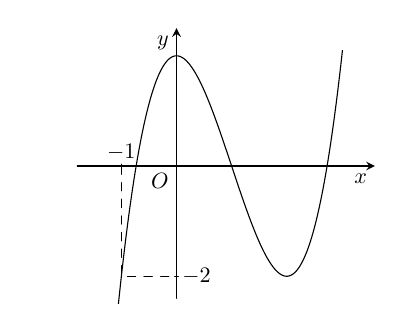
\begin{tikzpicture}[line join=round,line cap=round,>=stealth,scale=0.7]
		\tikzset{every  node/.style={scale=0.8}}
		\draw[->] (-1.8,0)--(3.6,0) node[below left]  {$x$};
		\draw[->]  (0,-2.4)--(0,2.5) node[below left] {$y$};
		\draw  (0,0) node [below left] {$O$};
		\foreach \x/\nx in  {-1/-1}
		 \draw[thin] (\x,1pt)--(\x,-1pt) node [above] {$\nx$};
		\foreach \y/\ny in  {-2/-2}
		\draw[thin] (1pt,\y)--(-1pt,\y) node [right] {$\ny$}; 
		\draw[dashed](-1,0)--(-1,-2)--(0,-2); 
		\begin{scope}
			\clip (-2.7,-2.5) rectangle (3.6,2.1); 
			\draw[samples=200,domain=-2:3.6,smooth,variable=\x] plot (\x,{1*(\x)^3-3*(\x)^2+2}); 
		\end{scope}
	\end{tikzpicture}
		 }
		{\True \begin{tikzpicture}[line join=round,line cap=round,>=stealth,scale=0.7]
		\tikzset{every  node/.style={scale=0.8}}
		 \draw[->] (-2.1,0)--(1.6,0) node[below left] {$x$};
		\draw[->] (0,-2.4)--(0,2.5)  node[below left] {$y$};
		\draw (0,0)  node [below left] {$O$};
		\foreach \x/\nx in {-1/-1} 
		\draw[thin] (\x,1pt)--(\x,-1pt) node  [below left] {$\nx$};
		\foreach \y/\ny in {-2/-2,1/1} 
		 \draw[thin] (1pt,\y)--(-1pt,\y) node [right] {$\ny$};
		 \draw[dashed](-1,0)--(-1,1)--(0,1);
		\begin{scope}
			\clip (-2.7,-2.5) rectangle  (3.6,2.1);
			\draw[samples=200,domain=-1:3.6,smooth,variable=\x]  plot (\x,{1*(\x)^3+3*(\x)^2-2});
			 \draw (-2,2)--(-1,1);
		\end{scope}
	\end{tikzpicture}
		 }
	 \loigiai{
		Xét  đồ thị
		\begin{center}
			\begin{tikzpicture}[>=stealth,x=1cm,y=1cm,scale=0.6]
					\draw[->,black]  (-2.2,0) -- (4,0) node[below] {$x$};
					\foreach \x in{-2,3} \draw[xshift=\x cm] (0pt,-2pt)--(0pt,2pt); 
					\draw[->,black]  (0,-2.5) -- (0,3.5) node[left] {$y$};
					\foreach \y  in{-2,-1,2,3} \draw[yshift=\y cm] (-2pt,0pt)--(2pt,0pt);
					\draw [-,black](-1,-2.5)--(-1,3.5); 
					 \draw (1,0) node[below]{$1$} circle (1pt);
					\draw (2,0) node[below]{$2$} circle  (1pt);
					\draw (-1,0) node[above left]{$-1$} circle  (1pt);
					\draw (0,1) node[left]{$1$} circle (1pt); 
					\draw (0,0) node[below right]{$O$} circle  (1pt);
					\draw [dashed] (1,0)--(1,1)--(0,1); 
					\draw[smooth,samples=100,domain=-0.8:3]  plot (\x,{ln((\x)+1)/ln(2)});
				\end{tikzpicture}0
		\end{center}
		Ta suy  ra $\lim\limits_{x\to -1^-}f(x)=1$ và $\lim\limits_{x\to -1^+}f(x)=0$.\\
		Suy ra $\lim\limits_{x\to -1^-}f(x)\ne  \lim\limits_{x\to -1^+}f(x)$.
	 }
\end{ex}

% từ: cau-hoi/lop11/1D3_Gioi_han_Ham_so_lien_tuc/1D3-3-2_Tinh_lien_tuc_the_hien_qua_do_thi.tex
\begin{ex}%[1D3B3-2]%[ma:280d4baf]
	Trong các dãy số được cho dưới đây, dãy số nào {\bf không}  phải là cấp số cộng?
	\choice 
		{ ${{u}_{n}}=-{{2}^{n}}+15$} 
		{ ${{u}_{n}}=-4n+9$} 
		 { ${{u}_{n}}=-2n-21$}
		 { \True ${{u}_{n}}=-2n+19$}
	\loigiai{ 
	Dãy số ${{u}_{n}}=-{{2}^{n}}+15$ không có dạng $an+b$ nên có không  phải là cấp số cộng.}
\end{ex}

% từ: cau-hoi/lop11/1D3_Gioi_han_Ham_so_lien_tuc/1D3-3-3_Ham_so_lien_tuc_tai_mot_diem.tex
\begin{ex}%[1D3N3-3]%[ma:ca12c85b]
	\immini[thm]{ 
	Hàm số $y=f(x)$ có đồ thị như  hình bên. Hàm số gián đoạn tại điểm có hoành độ bằng bao nhiêu?
	\choice 
		{$0$} 
		 {$2$}
		 {$3$}
		 {\True $1$}
		}{ 
		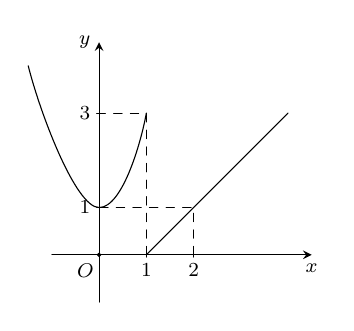
\begin{tikzpicture}[scale=0.6,font=\footnotesize,line join=round,line cap=round,>=stealth]
				\draw[->] (-1.0,0)  -- (4.5,0) node[below] {$x$};
				\foreach  \x in {1,2}
					{ 
				\draw (\x,-.05) -- (\x,.05); 
				 \draw (\x,0) node[below] {$\x$};}
				\draw[->] (0,-1.0) -- (0,4.5) node[left] {$y$}; 
				\foreach  \y in {1,3}
					{ 
				\draw (-.05,\y) -- (.05,\y); 
				\draw (0,\y) node[left]{$\y$}; 
				 }
				\draw 
					 (-1.5,4).. controls +(-76:1)
					and  +(180:.5)..(0,1).. controls +(0:.5)
					and +(-100:.6).. (1,3); 
				 \draw (1,0)--(4,3);
				\draw[dashed]  (1,0)|-(0,3)
					 (2,0)|-(0,1);
				\foreach \p/\q/\n/\g in {0/0/O/-130}\draw[fill] (\p,\q) circle (1pt)  node[shift={(\g:.3)}]{$\n$};
			\end{tikzpicture}
		 }
	\loigiai{ 
		 Dựa vào đồ thị của hàm số, ta thấy hàm số gián đoạn tại điểm có hoành độ bằng $1$.
	} 
\end{ex}

% từ: cau-hoi/lop11/1D3_Gioi_han_Ham_so_lien_tuc/1D3-3-4_Ham_so_lien_tuc_tren_khoang_doan.tex
\begin{ex}%[1D3K3-4]%[ma:1208e0c9]
	Biết các  số $\mathrm{C}_n^1$, $\mathrm{C}_n^2$, $\mathrm{C}_n^3$ theo thứ tự lập thành một cấp số cộng với $n>3$. Tìm $n$.
	\choice 
		{ $n=5$ } 
		 { $n=11$ }
		{  $n=9$ }
		{ \True  $n=7$ }
	 \loigiai{
		Ba số $\mathrm{C}_n^1$, $\mathrm{C}_n^2$, $\mathrm{C}_n^3$ theo thứ tự ${{u}_{1}},\,\,{{u}_{2}},\,\,{{u}_{3}}$ lập thành cấp số cộng nên 
		\begin{eqnarray*}
			&&{{u}_{1}}+{{u}_{3}}=2{{u}_{2}}\Leftrightarrow \mathrm{C}_n^1+\mathrm{C}_n^3=2\mathrm{C}_n^1\,\,(n\ge 3)\\ 
			 &\Leftrightarrow& n+\dfrac{(n-2)(n-1)n}{6}=2\cdot \dfrac{(n-1)n}{2}\Leftrightarrow 1+\dfrac{{{n}^2}-3n+2}{6}=n-1\\
			&\Leftrightarrow& {{n}^2}-9n+14=0\Leftrightarrow \hoac{ 
			& n=2  \\
			& n=7  \\
			}\Leftrightarrow  n=7\,(n\ge 3).
		\end{eqnarray*}
	\textbf{Nhận xét:}\\ Nếu ${{u}_{k-1}},\,\,{{u}_{k}},\,\,{{u}_{k+1}}$ là ba số hạng liên tiếp của một cấp số cộng thì  ta có ${{u}_{k-1}}+{{u}_{k+1}}=2{{u}_{k}}$.}
\end{ex}

% từ: cau-hoi/lop11/1D3_Gioi_han_Ham_so_lien_tuc/1D3-3-5_Bai_toan_phuong_trinh_co_nghiem.tex
\begin{ex}%[1D3H3-5]%[ma:7b98e1c5]
	Cho phương trình $2x^3-8x-1=0(1)$.  Khẳng định nào sai?
	\choice 
		{Phương  trình không có nghiệm lớn hơn $3$}
		{Phương trình có đúng $3$ nghiệm phân biệt} 
		{\True Phương trình có $2$ nghiệm lớn  hơn $2$}
		{Phương  trình có nghiệm trong khoảng $\left(-5;-1\right)$}
	 \loigiai{
		Hàm số $f(x)=2x^3-8x-1$ liên tục  trên $\mathbb{R}$.
		Do $f\left(-5\right)=-211$, $f\left(-1\right)=5> 0$, $f(2)=-1< 0$, $f(3)=29> 0$ nên phương trình có ít nhất $3$ nghiệm trên $\left(-5;-1\right)$,  $\left(-1;2\right)$, $\left(2;3\right)$.
		Mà phương trình bậc ba có tối đa $3$ nghiệm nên phương trình  có đúng $3$ nghiệm trên $\mathbb{R}$. Do đó C sai.
	} 
\end{ex}

% từ: cau-hoi/lop11/1D3_Gioi_han_Ham_so_lien_tuc/1D3-3-5_Bai_toan_phuong_trinh_co_nghiem.tex
\begin{ex}%[1D3H3-5]%[ma:89849a4f]
	Số nghiệm của phương  trình $x^3-3x-1=0$ là
	 \choice
		{$0$} 
		{\True $1$} 
		{$2$} 
		 {$3$}
	\loigiai{ 
		 Đặt $f(x)=x^3-3x-1$.\\
		Do $f(x)=x^3-3x-1$ là hàm đa thức có tập xác định là $\mathbb{R}$  nên liên tục trên $\mathbb{R}$.\\
		Do  đó hàm số liên tục trên mỗi khoảng $(-2;-1)$, $(-1;0)$, $(0;2)$.\\
		Ta có 
		\begin{itemize}
			\item $\heva{& f(-2)=-3 \\ & f(-1)=1} \Rightarrow f(-2)f(-1)<0 \Rightarrow$ phương trình đã cho có ít  nhất một nghiệm thuộc $(-2;-1).$
			\item $\heva{& f(-1)=1 \\ & f(0)=-1} \Rightarrow f(-1)f(0)<0 \Rightarrow$ phương trình đã cho có  ít nhất một nghiệm thuộc $(-1;0).$
			\item $\heva{& f(2)=1 \\ & f(0)=-1} \Rightarrow f(2)f(0)<0 \Rightarrow$ phương trình đã cho có ít nhất  một nghiệm thuộc $(0;2).$
		\end{itemize}
		Như vậy phương trình đã cho  có ít nhất ba thuộc khoảng $(-2;2)$.\\
		Tuy nhiên phương trình $f(x)=0$ là phương trình bậc ba có nhiều nhất  ba nghiệm.\\
		Vậy phương trình $f(x)=0$ có đúng $3$  nghiệm trên $\mathbb{R}$.
	} 
\end{ex}

% từ: cau-hoi/lop11/1D3_Gioi_han_Ham_so_lien_tuc/1D3-3-5_Bai_toan_phuong_trinh_co_nghiem.tex
\begin{bt}%[1D3V3-5]%[ma:43032179]
% nguon: Archive/SP_KhoLatex/ID6_old/15-OT-GioiHan-LienTuc.tex #2702
%[DGNL-DGTD-2022]%[Huỳnh Xuân Tín]
	Chứng minh phương trình $\left(m^2+1\right) x^3-2 m^2x^2-4 x+m^2+1=0$ có ba nghiệm phân biệt.
	\loigiai{
		Đặt $f(x) = \left(m^2+1\right) x^3-2 m^2x^2-4 x+m^2+1$, $f(x)$ liên tục với mọi $x \in \mathbb{R}$.\\
		Xét 
		\[f(-3) = \left(m^2+1\right) \cdot (-3)^3-2 m^2 \cdot (-3)^2-4 \cdot (-3)+m^2+1 = -44m^2 - 14<0.\]
		Xét 
		\[f(0) = \left(m^2+1\right) \cdot 0^3-2 m^2 \cdot 0^2-4 \cdot 0+m^2+1 = m^2+1>0.\]
		Xét 
		\[f(1) = \left(m^2+1\right) \cdot 1^3-2 m^2 \cdot 1^2-4 \cdot 1+m^2+1 = -2 < 0.\]
		Xét 
		\[f(2) = \left(m^2+1\right) \cdot 2^3-2 m^2 \cdot 2^2-4 \cdot 2+m^2+1 = m^2+1>0.\]
		Ta thấy $f(-3) \cdot f(0) < 0$, $f(0) \cdot f(1) <0$, $f(1) \cdot f(2) < 0$ nên phương trình $\left(m^2+1\right) x^3-2 m^2x^2-4 x+m^2+1=0$ có ít nhất $1$ nghiệm trong khoảng $(-3;0)$, ít nhất $1$ nghiệm trong khoảng $(0;1)$, ít nhất $1$ nghiệm trong khoảng $(1;2)$.\\
		Vậy phương trình $\left(m^2+1\right) x^3-2 m^2x^2-4 x+m^2+1=0$ có ba nghiệm phân biệt.
	}
\end{bt}

% từ: cau-hoi/lop11/1D3_Gioi_han_Ham_so_lien_tuc/1D3-3-5_Bai_toan_phuong_trinh_co_nghiem.tex
\begin{bt}%[1D3H3-5]%[ma:13559e87]
% nguon: Archive/SP_KhoLatex/ID6_old/1K5-17.tex #2836
%[Dự án 2 - TLDH - TeamTeXHoa - Nguyễn Thắng]
	Chứng minh rằng các phương trình sau có $3$ nghiệm phân biệt:
	\begin{enumerate}
		\item $x^3-3 x+1=0$
		\item $2 x+6 \sqrt[3]{1-x}=3$
	\end{enumerate}
	\loigiai
	{\begin{enumerate}
			\item Dễ thấy hàm $f(x)=x^3-3 x+1$ liên tục trên $\mathbb{R}$.\\
			Ta có
			\begin{itemize}
				\item  $\heva{&(-2)=-1 \\& f(-1)=3} \Rightarrow f(-2) \cdot f(-1)<0\\ \Rightarrow$ tồn tại một số $a_1 \in(-2 ;-1): f(a_1)=0\quad(1)$.
				\item $\heva{&f(0)=1 \\& f(1)=-1} \Rightarrow f(0) \cdot f(1)<0 \Rightarrow$ tồn tại một số $a_2 \in(0 ; 1): f\left(a_2\right)=0\quad(2)$.
				\item $\heva{&f(1)=-1 \\& f(2)=3} \Rightarrow f(1) \cdot f(2)<0 \Rightarrow$ tồn tại một số $a_3 \in(1 ; 2): f\left(a_3\right)=0\quad(3)$.
			\end{itemize}
			Từ (1), (2), (3) và ba khoảng $(-2 ;-1)$, $(0 ; 1)$ và $(1 ; 2)$ đôi một không giao nhau nên phương trình $x^3-3 x+1=0$ có ít nhất $3$ nghiệm phân biệt.\\
			Mà phương trình bậc $3$ thì chỉ có tối đa là $3$ nghiệm nên $x^3-3 x+1=0$ có đúng $3$ nghiệm phân biệt.
			\item  Đặt $\sqrt[3]{1-x}=t \Leftrightarrow x=1-t^3 \Rightarrow 2 t^3-6 t+1=0$.\\
			Xét hàm số $f(t)=2 t^3-6 t+1$ liên tục trên $\mathbb{R}$.\\
			Ta có $\heva{&f(-2) \cdot f(-1)=-3 \cdot 5<0 \\& f(0) \cdot f(1)=1 \cdot(-3)<0 \\& f(1) \cdot f(2)=-3 \cdot 5<0} \Rightarrow$ tồn tại $3$ số $t_1$, $t_2$ và $t_3$ lần lượt thuộc $3$ khoảng đôi một không giao nhau là $(-2 ;-1)$, $(0 ; 1)$ và $(1 ; 2)$ sao cho $f\left(t_1\right)=f\left(t_2\right)=f\left(t_3\right)=0$ và do đây là phương trình bậc $3$ nên $f(t)=0$ có đúng $3$ nghiệm phân biệt.\\
			Ứng với mỗi giá trị $t_1$, $t_2$ và $t_3$ ta tìm được duy nhất một giá trị $x$ thỏa mãn $x=1-t^3$ và hiển nhiên $3$ giá trị này khác nhau nên PT ban đầu có đúng $3$ nghiệm phân biệt.	
		\end{enumerate}
	}
\end{bt}

% từ: cau-hoi/lop11/1D3_Gioi_han_Ham_so_lien_tuc/1D3-3-5_Bai_toan_phuong_trinh_co_nghiem.tex
\begin{bt}%[1D3H3-5]%[ma:afc9fe58]
% nguon: Archive/SP_KhoLatex/ID6_old/1K5-17.tex #2837
%[Dự án 2 - TLDH - TeamTeXHoa - Nguyễn Thắng]
	Chứng minh rằng các phương trình sau luôn có nghiệm:
	\begin{enumerate}
		\item $x^5-3 x+3=0$.
		\item $x^4+x^3-3 x^2+x+1=0$.
	\end{enumerate}
	\loigiai
	{\begin{enumerate}
			\item Xét $f(x)=x^5-3 x+3$.\\
			Ta có
			$\lim\limits_{x \rightarrow+\infty} f(x)=+\infty \Rightarrow$ tồn tại một số $x_1>0$ sao cho $f\left(x_1\right)>0$.\\
			Và $\lim\limits_{x \rightarrow-\infty} f(x)=-\infty \Rightarrow$ tồn tại một số $x_2<0$ sao cho $f\left(x_2\right)<0$.\\
			Từ đó $f\left(x_1\right) \cdot f\left(x_2\right)<0 \Rightarrow$ luôn tồn tại một số $x_0 \in\left(x_2 ; x_1\right): f\left(x_0\right)=0$ nên phương trình $x^5-3 x+3=0$ luôn có nghiệm.
			\item Xét $f(x)=x^4+x^3-3 x^2+x+1$ liên tục trên $\mathbb{R}$\\
			Ta có $f(-1)=-3<0$,
			$\lim\limits_{x \rightarrow+\infty} f(x)=+\infty \Rightarrow$ tồn tại một số $a>0$ sao cho $f(a)>0$.\\
			$\Rightarrow x^2-x-3=0$ nên luôn tồn tại một số $x_0 \in(0 ; a)$ thỏa mãn $f\left(x_0\right)=0$ nên phương trình $x^4+x^3-3 x^2+x+1=0$ luôn có nghiệm.	
		\end{enumerate}
	}
\end{bt}

% từ: cau-hoi/lop11/1D5_Cac_so_dac_trung_do_xu_the_trung_tam_cho/1D5-1-1_Cau_hoi_ly_thuyet.tex
\begin{ex}%[1D5Y1-1]%[ma:5868a78d]
	Cho hàm số $ f\left( x \right)  $ liên tục trên khoảng $ (a;b) $, $ x_0 \in (a;b) $. Tính $ f'\left( x_0 \right) $ bằng định nghĩa ta cần tính
	 \choice
		 {$ \mathop {\lim }\limits_{x \to 0} \dfrac{{\Delta y}}{{\Delta x}} $}
		 {\True $ \mathop {\lim }\limits_{\Delta x \to 0} \dfrac{{\Delta y}}{{\Delta x}} $}
		{$ \mathop {\lim }\limits_{\Delta x \to 0}  \dfrac{{\Delta x}}{{\Delta y}} $}
		{$ \mathop {\lim }\limits_{x \to 0}  \dfrac{{\Delta y}}{{x}} $}
	\loigiai{ 
		Theo định nghĩa đạo hàm ta có  $ f'\left( x_0 \right) = \mathop {\lim }\limits_{\Delta x \to 0} \dfrac{{\Delta y}}{{\Delta x}} $.
	} 
\end{ex}

% từ: cau-hoi/lop11/1D5_Cac_so_dac_trung_do_xu_the_trung_tam_cho/1D5-2-1_Cau_hoi_ly_thuyet.tex
\begin{ex}%[1D5K2-1]%[ma:eeeaed18]
	Biết đạo hàm của hàm số $y=\dfrac{x-1}{\sqrt{x^{2}+1}}$ là $y'=\dfrac{ax+b}{\sqrt{\left(x^{2}+1\right)^{c}}}$ với $a$, $b$, $c$ là các số nguyên dương. Khi đó giá trị của $2a+b+c$ bằng: 
	\choice 
		 {$5$}
		 {\True $6$}
		{$7$} 
		{$4$} 
	 \loigiai{
		Ta có $y\cdot \sqrt{x^2+1} = x-1$.\\ 
		Lấy đạo hàm hai vế ta có $y'\sqrt{x^2+1}+y\cdot \left(\sqrt{x^2+1}\right)'=1 \Leftrightarrow y'\sqrt{x^2+1}+y\cdot  \dfrac{x}{\sqrt{x^2+1}}=1$.\\
		Suy ra  $y'\sqrt{x^2+1}=1-y\cdot \dfrac{x}{\sqrt{x^2+1}}=1-\dfrac{x^2-x}{x^2+1} = \dfrac{x+1}{x^2+1}$\\
		$\Rightarrow y'  = \dfrac{x}{(x^2+1)\sqrt{x^2+1}}=\dfrac{x}{\sqrt{(x^2+1)^3}}$.\\
		Vậy $a=1,b=0,c=3  \Rightarrow 2a+b+c=6$.
	 }
\end{ex}

% từ: cau-hoi/lop11/1D5_Cac_so_dac_trung_do_xu_the_trung_tam_cho/1D5-2-1_Cau_hoi_ly_thuyet.tex
\begin{ex}%[1D5B2-1]%[ma:0bcd9141]
	Đạo hàm của hàm số $f(x)=5x^3-x^2-1$ trên khoảng $(-\infty;+\infty)$ là 
	 \choice
		{$0$} 
		{$15x^2-2x-1$} 
		 {$15x^2+2x$}
		{\True $15x^2-2x$} 
	\loigiai{Ta  có
		$f'(x)=5\cdot  3x^2-2x=15x^2-2x$.
	} 
\end{ex}

% từ: cau-hoi/lop11/1D5_Cac_so_dac_trung_do_xu_the_trung_tam_cho/1D5-2-1_Cau_hoi_ly_thuyet.tex
\begin{ex}%[1D5B2-1]%[ma:24048ead]
	Cho hàm số $f(x)=x^3-2x^2+x-4$. Biết tập nghiệm của bất phương  trình $f'(x)\le 0$ là đoạn $[a;b]$. Tính $P=3a-4b$.
	\choice 
		 {\True $ -3 $}
		{$ -1  $}
		{$  25 $}
		{$  -\dfrac{5}{3} $}
	\loigiai{ 
		Ta có $f'(x)=3x^2-4x+1$.\\ 
		$f'(x)\le  0 \Leftrightarrow x\in \left[\dfrac{1}{3};1\right]$.\\
		Khi đó $a=\dfrac{1}{3}$,  $b=1$.\\
		 Vậy $P=3a-4b=1-4=-3$.
	} 
\end{ex}

% từ: cau-hoi/lop11/1D5_Cac_so_dac_trung_do_xu_the_trung_tam_cho/1D5-2-1_Cau_hoi_ly_thuyet.tex
\begin{ex}%[1D5Y2-1]%[ma:aabdd9f8]
	Hàm số $y=\sqrt{x^4+1}$ có đạo  hàm $y'$ bằng
	\choice 
		{$\dfrac{1}{\sqrt{x^4+1}}$} 
		{$\dfrac{4x^3}{\sqrt{x^4+1}}$} 
		{\True  $\dfrac{2x^3}{\sqrt{x^4+1}}$}
		 {$\dfrac{x^4}{2\sqrt{x^4+1}}$}
	 \loigiai{
	Ta  có $y'=\dfrac{(x^4+1)'}{2\sqrt{x^4+1}}=\dfrac{4x^3}{2\sqrt{x^4+1}}=\dfrac{2x^3}{\sqrt{x^4+1}}$.
	 }
\end{ex}

% từ: cau-hoi/lop11/1D5_Cac_so_dac_trung_do_xu_the_trung_tam_cho/1D5-2-1_Cau_hoi_ly_thuyet.tex
\begin{ex}%[1D5Y2-1]%[ma:a406ffca]
	Tính đạo hàm  của hàm số $y=x+\cot x-3 $.
	\choice 
		{$y'=1+\dfrac 1{\sin^2x}$} 
		 {\True $y'=1-\dfrac 1{\sin^2x}$}
		{$y'=1-\dfrac 1{\cos^2x}$} 
		{$y'=1+\dfrac  1{\cos^2x}$}
	\loigiai{ 
		Ta  có $y'=(x+\cot x-3)'=1-\dfrac 1{\sin^2x}$.
	 }
\end{ex}

% từ: cau-hoi/lop11/1D5_Cac_so_dac_trung_do_xu_the_trung_tam_cho/1D5-2-2_Trung_vi.tex
\begin{ex}%[1D5Y2-2]%[ma:5d7cb405]
	Hệ số góc $k$ của tiếp tuyến  đồ thị hàm số $y = x^3 + 1$ tại điểm $M(1; 2)$ là
	 \choice
		 {$k = 12$}
		 {\True $k = 3$}
		 {$k = 5$}
		{$k  = 4$}
	\loigiai{Ta có $y' =  3x^2$. Tại điểm $M$ có hoành độ $x = 1$ thì $k = y'(1) = 3\cdot 1^2 = 3$.
	 }
\end{ex}

% từ: cau-hoi/lop11/1D5_Cac_so_dac_trung_do_xu_the_trung_tam_cho/1D5-2-2_Trung_vi.tex
\begin{ex}%[1D5Y2-2]%[ma:46ebce40]
	Nếu hàm số $y=f\left( {x} \right)$ có đạo hàm tại  $x_0$ thì phương trình tiếp tuyến của đồ thị hàm số tại điểm $M_0\left( {x_0;f\left( {x_0} \right)} \right)$ là
	 \choice
		 {$y=f'\left( {x} \right)\left( {x-x_0} \right)+f\left( {x_0} \right)$}
		{$y=f'\left( {x}  \right)\left( {x-x_0} \right)-f\left( {x_0} \right)$}
		{\True $y=f'\left(  {x_0} \right)\left( {x-x_0} \right)+f\left( {x_0} \right)$}
		{$y=f'\left( {x_0} \right)\left(  {x-x_0} \right)-f\left( {x_0} \right)$}
	\loigiai{Theo ý nghĩa hình học của đạo hàm, phương  trình tiếp tuyến của đồ thị hàm số tại điểm $M\left( {x_0;f\left( {x_0} \right)} \right)$ là $y=f'\left( {x_0} \right)\left( {x-x_0} \right)+f\left( {x_0} \right)$.}
\end{ex}

% từ: cau-hoi/lop11/1D6_Ham_so_mu_va_ham_so_logarit/1D6-1-1_Tinh_gia_tri_cua_bieu_thuc_chua_luy_thua.tex
\begin{bt}%[1D6H1-1]%[ma:37482be7]
	Biết  $4^x+4^{-x}=23$, tính giá trị biểu thức $P=2^x+2^{-x}$.
	 \loigiai{
		Đặt $P=2^x+2^{-x} \Rightarrow P >  0$.\\
		Ta có  $P^2=\left(2^x+2^{-x} \right)^2=4^x+4^{-x}+2\cdot 2^x \cdot 2^{-x}=23+2=25$.\\
		Do đó  $P=5$.
	 }
\end{bt}

% từ: cau-hoi/lop11/1D6_Ham_so_mu_va_ham_so_logarit/1D6-2-2_Bien_doi_bieu_dien_bieu_thuc_chua_logarit.tex
\begin{ex}%[1D6V2-2]%[ma:369cc583]
 Cho hàm số $y = x + \dfrac{4}{x -  3}$ có đồ thị $(C)$ và đường thẳng $d\colon y = -3x + 2$. Khi đó
 \choiceTF 
  {Điểm $N(-1;0)$ thuộc đồ thị $(C)$} 
  {Đồ thị $(C)$ và đường thẳng $d$ cắt nhau tại hai điểm có tích hoành độ giao  điểm bằng $-\dfrac{5}{2}$}
  {\True Tiếp  tuyến của đồ thị $(C)$ tại điểm có hoành độ bằng $1$ song song với trục hoành}
  {\True $M_1(2;-2),M_2(4;8)$ là hai điểm thuộc đồ thị $(C)$ mà tiếp tuyến của $(C)$ tại đó song song với đường thẳng $d$} 
 \loigiai{ 
  \begin{itemchoice}
   \itemch  Sai.\\
   Với $x=-1$  thì $y=-2$ nên điểm $N(-1;0)$ không thuộc đồ thị $(C)$.
   \itemch Sai\\ 
   Phương trình hoành độ giao điểm của $(C)$ và $(d)$  là
   \begin{eqnarray*}
     && x + \dfrac{4}{x - 3}=-3x+2\\
    &\Leftrightarrow &  \heva{&x\ne 3\\&4x-2+\dfrac{4}{x-3}=0}\\
    &\Leftrightarrow  & \heva{& x\ne 3\\& (4x-2)(x-3)+4=0}\\
    &\Leftrightarrow & \heva{&x\ne 3\\&2x^2-7x+5=0.} 
   \end{eqnarray*}
   Phương trình này có $\Delta=9>0$ nên có hai nghiệm. Theo định lý Viète tích hai  nghiệm bằng $\dfrac{5}{2}$.
   \itemch Đúng.\\ 
   Với $x=1$ thì $y=-1$ nên  điểm $K(1;-1)$ không thuộc trục $Ox$.\\
   Lại có $y'=1-\dfrac{4}{(x-3)^2}$ nên  $y'(1)=0$. Do đó tiếp tuyến của $(C)$ tại $K(1;-1)$ song song với trục hoành.
   \itemch Đúng.\\ 
   Đặt $f(x)=x +  \dfrac{4}{x - 3}$.
   Ta có $f'(x) = 1 - \dfrac{4}{\left(x - 3 \right)^2}$. \\ 
   Gọi $M\left(x_0; f\left(x_0 \right)  \right)$ là tọa độ tiếp điểm. \\
   Hệ số góc của tiếp tuyến tại điểm $\left(x_0; f\left(x_0 \right) \right)$ là $y'(x_0)  = \dfrac{x^2_0 - 6x_0 + 5}{\left(x_0 - 3 \right)^2}$. \\
   Vì tiếp tuyến song song với đường thẳng $d:y = -3x +  2 $ nên
   $$y'(x_0) = - 3 \Leftrightarrow \heva{&4x^2_0 - 24x_0 + 32 = 0 \\ &x_0 \neq 3}  \Leftrightarrow \hoac{&x_0 = 4 \\ &x_0 = 2.}$$
   Với $x_0=2$, suy ra  tiếp điểm $M_1(2;-2)$ và $f'(2)=-3$. Phương trình tiếp tuyến tại $M_1$ là
   \[y+2=-3(x-2)\Leftrightarrow  y=-3x+4.\]
    Với $x_0=4$, suy ra tiếp điểm $M_2(4;8)$ và $f'(4)=-3$. Phương trình tiếp tuyến tại $M_1$ là
    \[y-8=-3(x-4)\Leftrightarrow y=-3x+20.\]
   Cả hai tiếp  tuyến đều song song với đường thẳng $d$. Suy ra có hai tiếp điểm thỏa yêu cầu bài $M_1(2;-2),M_2(4;8)$.
  \end{itemchoice}
  }
\end{ex}

% từ: cau-hoi/lop11/1D6_Ham_so_mu_va_ham_so_logarit/1D6-3-1_Cau_hoi_ly_thuyet_ham_so_luy_thua_mu_logarit.tex
\begin{ex}%[1D6N3-1]%[ma:e8ac35e6]
	Cho $a$ là  số thực dương và khác $1$. Mệnh đề nào sau đây là \textbf{sai}?
	 \choice
		{$\log_a\left(\dfrac{x}{y}\right)=\log_a x-\log_a y,\forall  x>0,y>0$}
		{$\log_a(xy)=\log_a  x+\log_a y,\forall x>0,y>0$}
		 {\True $\log_a x^2=\dfrac{1}{2}\log_a x,\forall x>0$}
		{$\log a=\dfrac{1}{\log_a 10}$} 
	\loigiai{Với $0<a\neq 1$, $x>0$ ta có $\log_a  x^2=2\log_a x$ nên mệnh đề $\log_a x^2=\dfrac{1}{2}\log_a x,\forall x>0$ sai.}
\end{ex}

% từ: cau-hoi/lop11/1D6_Ham_so_mu_va_ham_so_logarit/1D6-3-4_So_sanh_cac_luy_thua_va_logarit.tex
\begin{ex}%[1D6H3-4]%[ma:89255772]
	Cho $a$ và $b$ là các số thực dương tùy ý. Nếu $a^2>a^3$ và  $\log_b\dfrac{1}{3}<\log_b\dfrac{1}{4}$ thì
	 \choice
		{\True  $a>1$, $0<b<1$}
		{$0<a<1$,  $0<b<1$}
		{$a>1$, $b>1$} 
		 {$0<a<1$, $b>1$}
	\loigiai{ 
		Ta có $\dfrac{1}{2}>\dfrac{1}{3}$  mà $a^2>a^3$ nên $a>1$.\\
		Mặt khác, $\dfrac{1}{3}>\dfrac{1}{4}$ mà  $\log_b\dfrac{1}{3}<\log_b\dfrac{1}{4}$ nên $0<b<1$.
	} 
\end{ex}

% từ: cau-hoi/lop11/1D6_Ham_so_mu_va_ham_so_logarit/1D6-4-2_Phuong_trinh_mu_logarit_co_ban.tex
\begin{ex}%[1D6H4-2]%[ma:2a520207]
	 Cho $a$, $b$, $c$ là ba số dương khác $1$. Đồ thị các hàm số $y=\log_a x$, $y=\log_b x$, $y=\log_c x$ được cho trong hình vẽ bên.
	\begin{center}
		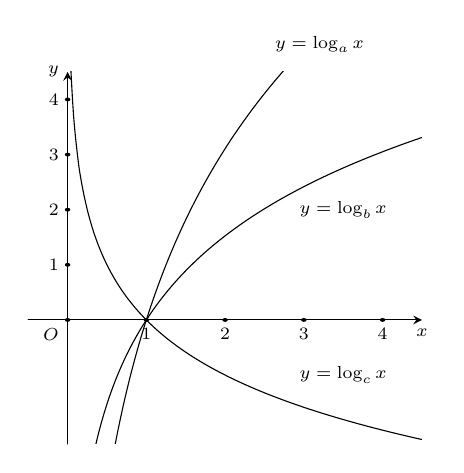
\begin{tikzpicture}[scale=1,>=stealth,font=\scriptsize,line join=round,line cap=round,yscale=.7]
				\draw[->] (-0.5,0)--(4.5,0) node[below] {$x$}; 
				\draw[->] (0,-2.25)--(0,4.5) node[left] {$y$}; 
				\fill (0,0) circle (1pt) node[below  left]{$O$};
				\node at (3.2,5) {$y=\log_a  x$};
				\node at (3.5,2) {$y=\log_b  x$};
				\node at (3.5,-1) {$y=\log_c x$}; 
				\clip (-0.5,-2.25)  rectangle (4.5,4.5);
				\foreach  \x in {1,2,3,4}{\fill (\x,0) circle (1pt) node[below]{$\x$};}
				\foreach \y in {1,2,3,4}{\fill (0,\y) circle (1pt) node[left]{$\y$};} 
				 \draw[domain=0.01:4.5,samples=200,smooth]
					plot (\x,{ln (\x)/ln  (1.25)});
				 \draw[domain=0.01:4.5,samples=200,smooth]
					 plot (\x,{ln (\x)/ln (3.91^(1/3))});
				 \draw[domain=0.01:4.5,samples=200,smooth]
					plot (\x,{ln (\x)/ln  (0.5)});
			\end{tikzpicture}
	\end{center}
	\choiceTF 
		{\True Trong các hàm số $y=\log_a x$, $y=\log_b x$, $y=\log_c x$ (đồ thị trên hình vẽ), có đúng hai hàm số đồng biến trên các  tập xác định của nó}
		{\True $\log_c x > \log_c 2  \Rightarrow x<2$}
		 {$c<b<a$}
		{Đường thẳng $y=3$ cắt trục $Oy$ và cắt đồ  thị các hàm số $y=\log_a x$, $y=\log_b x$ lần lượt tại các điểm $M$, $N$, $P$ sao cho $N$ là trung điểm của $MP$. Khi đó $a^3=2b^3$}
	\loigiai{ 
		\begin{itemchoice}
			\itemch Hàm số $y=\log_a x$, $y=\log_b x$ đồng  biến, $y=\log_c x$ nghịch biến.
			\itemch Hàm $y=\log_c  x$ nghịch biến nên $\log_c x > \log_c 2 \Rightarrow x<2$.
			\itemch Vì $y=\log_a x$, $y=\log_b x$ đồng biến, nên $a>1$, $b>1$.\\ Vì $y=\log_c x$ nghịch biến, nên $0<c<1$. Kẻ đường $y=1$ cắt  các đồ thị, ta thấy hoành độ của giao điểm với $y=\log_a x$ nhỏ hơn của $y=\log_b x$, tức là $a<b$.\\
			 Vậy $c<a<b$.
			 \itemch
			\begin{center}
				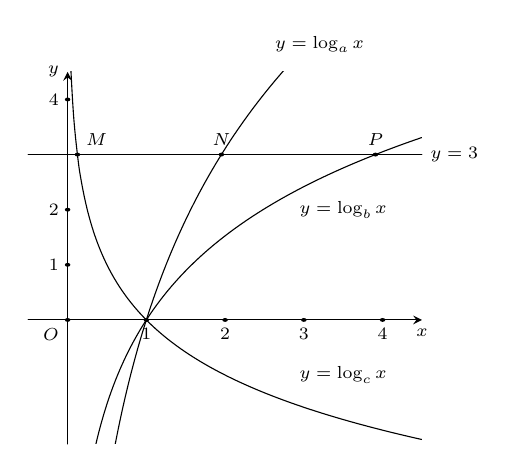
\begin{tikzpicture}[scale=1,>=stealth,font=\scriptsize,line join=round,line cap=round,yscale=.7]
						\draw[->]  (-0.5,0)--(4.5,0) node[below] {$x$};
						\draw[->] (0,-2.25)--(0,4.5) node[left]  {$y$};
						 \fill (0,0) circle (1pt) node[below left]{$O$};
						\node at (3.2,5) {$y=\log_a x$}; 
						\node at (3.5,2) {$y=\log_b x$}; 
						\node at (3.5,-1)  {$y=\log_c x$};
						\draw (-0.5,3)--(4.5,3) node[right]{$y=3$}; 
						\fill ({0.5^3},3) circle (1pt)  node[above right]{$M$}
						({1.25^3},3) circle (1pt) node[above]{$N$} 
						(3.91,3)  circle (1pt) node[above]{$P$};
						\clip (-0.5,-2.25) rectangle (4.5,4.5); 
						 \foreach \x in {1,2,3,4}{\fill (\x,0) circle (1pt) node[below]{$\x$};}
						\foreach \y in {1,2,4}{\fill  (0,\y) circle (1pt) node[left]{$\y$};}
						 \draw[domain=0.01:4.5,samples=200,smooth]
						 plot (\x,{ln (\x)/ln (1.25)});
						\draw[domain=0.01:4.5,samples=200,smooth] 
						plot (\x,{ln  (\x)/ln (3.91^(1/3))});
						\draw[domain=0.01:4.5,samples=200,smooth] 
						plot (\x,{ln (\x)/ln (0.5)}); 
					\end{tikzpicture}
			\end{center}
			Đường thẳng $y=3$ cắt trục $Oy$ và cắt đồ  thị các hàm số $y=\log_a x$, $y=\log_b x$ lần lượt tại các điểm $M(0;3)$, $N(a^3;3)$, $P(b^3;3)$.\\
			Vì $N$ là trung điểm của $MP$ nên \[x_N=\dfrac{x_M+x_P}{2} \Leftrightarrow  a^3=\dfrac{0+b^3}{2} \Leftrightarrow 2a^3=b^3.\]
		\end{itemchoice}
	} 
\end{ex}

% từ: cau-hoi/lop11/1D6_Ham_so_mu_va_ham_so_logarit/1D6-4-3_Bat_phuong_trinh_mu_logarit_co_ban.tex
\begin{ex}%[1D6H4-3]%[ma:79497fb3]
	Cho các số thực $a$, $b$ thỏa mãn $a>b>1$ và $\dfrac{1}{\log_{b} a}+\dfrac{1}{\log_{a} b}=\sqrt{2023}$. Giá trị của biểu thức $P=\dfrac{1}{\log_{ab} b}-\dfrac{1}{\log_{ab} a}$ bằng (kết quả làm  tròn đến hàng phần mười)
	 \shortans{44,9}
	\loigiai{ 
		Do $a>b>1$  nên $\log_{b} a > 0$, $\log_{a} b > 0$ và $\log_{b} a > \log_{a} b$. \\
		Ta  có
		\begin{align*}
			 \dfrac{1}{\log_{b} a} + \dfrac{1}{\log_{a} b} = \sqrt{2023}
			&\Leftrightarrow \log_{a} b  + \log_{b} a = \sqrt{2023}\\
			&\Leftrightarrow \log_{a}^2  b + \log_{b}^2 a + 2 = 2023\\
			&\Leftrightarrow  \log_{a}^2 b + \log_{b}^2 a = 2021
		\end{align*}
		Khi  đó,
		\begin{align*}
			P &= \log_{b} ab - \log_{a}  ab \\
			&= \log_{b} a + \log_{b} b  - \log_{a} a - \log_{a} b \\
			&=  \log_{b} a - \log_{a} b
		\end{align*}
		Suy  ra
		$$ 
		P^2 =(\log_{b} a - \log_{a} b)^2 = \log_{b}^2 a + \log_{a}^2  b - 2 = 2021 - 2 = 2019.
		$$ 
		Vậy, $P =  \sqrt{2019}$.
	} 
\end{ex}

% từ: cau-hoi/lop11/1D6_Ham_so_mu_va_ham_so_logarit/1D6-4-4_Phuong_trinh_mu_logarit_dua_ve_cung_co_so.tex
\begin{ex}%[1D6V4-4]%[ma:4d0ebeb1]
	Cho phương trình $9^x-(m-1)\cdot  3^x-m-1=0\quad(*)$ với $m$ là tham số.
	 \choiceTF
		{Phương trình $(*)$ có thể  có $3$ nghiệm}
		{Khi $m=0$ phương  trình $(*)$ có hai nghiệm trái dấu}
		{Khi $m=1$ phương  trình $(*)$ có hai nghiệm phân biệt}
		{\True Số giá trị nguyên của $m$ để phương trình $(*)$ có hai nghiệm phân  biệt là $0$}
	\loigiai{ 
		\begin{itemchoice}
			 \itemch
			Đặt $t=3^x$, $t>0$ khi  đó $(*)$ trở thành $t^2-\left(m-1\right)t-m-1=0\quad(**)$.\\
			Phương trình $(**)$ là phương trình bậc hai theo $t$ nên có thể có nhiều nhất là hai nghiệm $t$, mà $t=3^x$ nên một giá trị $t$ có thể cho nhiều nhất một nghiệm $x$. Vậy  phương trình $(*)$ có thể có nhiều nhất là hai nghiệm.
			 \itemch
			Khi $m=0$ phương  trình trở thành $9^x+3^x-1=0$.\\
			Đặt  $t=3^x$, $t>0$ khi đó $(*)\Rightarrow t^2+t-1=0\quad(1)$.\\
			Theo định lí Vi-et thì phương trình $(1)$ có hai nghiệm trái dấu nên có một  nghiệm dương từ đó suy ra phương trình $(*)$ có một nghiệm $x$ khi $m=0$.
			\itemch 
			Khi $m=1$ phương trình  trở thành $9^x-2=0\Leftrightarrow x=\log_9 2$.
			\itemch 
			Đặt $t=3^x$, $t>0$ khi đó $(*)\Rightarrow t^2-(m-1)t-m-1=0 \quad(2)$.\\ 
			Phương trình $(*)$ có hai nghiệm phân biệt  khi và chỉ khi phương trình $(2)$ phải có hai nghiệm dương $t_1$, $t_2$ phân biệt
			\begin{eqnarray*}
				\Leftrightarrow \heva{&\Delta  > 0\\& S=t_1+t_2 > 0\\&P=t_1 \cdot t_2 > 0} &\Leftrightarrow &\heva{&(m+1)^2+4> 0\\& m-1> 0\\& -m-1> 0}\\
				 &\Leftrightarrow & \heva{& m > 1\\& m <-1} \Leftrightarrow m\in \varnothing.
			\end{eqnarray*}
			Từ  đó suy ra không có giá trị nguyên của $m$ để phương trình có hai nghiệm phân biệt.
		\end{itemchoice}
	} 
\end{ex}

% từ: cau-hoi/lop11/1D6_Ham_so_mu_va_ham_so_logarit/1D6-4-4_Phuong_trinh_mu_logarit_dua_ve_cung_co_so.tex
\begin{ex}%[1D6V4-4]%[ma:86503d1d]
	Cho  phương trình $4^x-m\cdot 2^{x+1}+2m=0\quad(1)$
	 \choiceTF
		{\True Khi đặt $2^x=t>0$, phương trình $(1)$ trở thành phương trình $t^2-2m\cdot  t+2m=0$}
		 {Khi $m=0$ phương trình $(1)$ có hai nghiệm trái dấu}
		{Phương trình $4^x-m\cdot 2^{x+1}+2m=0$ có hai nghiệm phân  biệt khi và chỉ khi $m\ge 2$}
		{Phương trình $4^x-m\cdot 2^{x+1}+2m=0$ có hai nghiệm $x_1$, $x_2$ với thỏa mãn $x_1+x_2=3$  khi $m\in (4;5)$}
	\loigiai{ 
		\begin{itemchoice}
			\itemch Khi đặt $2^x=t>0$, phương trình $(1)$  trở thành phương trình $t^2-2m\cdot t+2m=0$
			 \itemch
			Khi $m=0$ phương trình $(1)$ trở thành $4^x=0$, phương  trình vô nghiệm.
			 \itemch
			Đặt  $2^x=t>0$, phương trình $(1)$ trở thành phương trình $t^2-2m\cdot t+2m=0\quad(2)$.\\
			$(1)$ có $2$ nghiệm phân  biệt khi $(2)$ có $2$ nghiệm dương phân biệt. Khi đó
			\[\heva{&\Delta'=(-m)^2-2m=m^2-2m>0\\&S=2m>0\\& P=2m > 0}  \Leftrightarrow m > 2.\]
			 \itemch
			Ta có $x_1+x_2=3$ hay  $2^{x_1+x_2}=2^3$.\\
			Đặt $2^x=t > 0$, phương trình $(1)$  trở thành phương trình $t^2-2mt+2m=0\quad(2)$.\\
			Suy ra  ta cần tìm $m$ để phương trình $(2)$ có hai nghiệm $t_1$, $t_2$ thỏa mãn $t_1\cdot t_2=8$.\\ Theo viet ta có $t_1\cdot t_2=8=2m\Leftrightarrow m=4$.\\ Thử lại ta được $m=4$ thỏa mãn.
		\end{itemchoice}
	} 
\end{ex}

% từ: cau-hoi/lop11/1D6_Ham_so_mu_va_ham_so_logarit/1D6-4-5_Bat_phuong_trinh_mu_logarit_dua_ve_cung_co_so.tex
\begin{ex}%[1D6H4-5]%[ma:4996087d]
	Số tự nhiên $3^{2023}$ có bao nhiêu chữ số? 
	\shortans{966} 
	\loigiai{ 
		Đặt $n=3^{2023} \Rightarrow \log n=2023 \log  3 \approx 965,216$.\\
		Suy ra $965<\log n<966 \Rightarrow  10^{965}<n<10^{966}$.\\
		Ta biết  $10^{965}$ có 966 chữ số nên $10^{966}$ có $967$ chữ số mà $n\in(10^{965}; 10^{966})$ nên có $966$ giá trị của $n$.\\
		Lưu ý $10^n \Rightarrow n+1$ chữ số. Ví dụ $10^2=100 \Rightarrow 2+1$ chữ  số.
	 }
\end{ex}

% từ: cau-hoi/lop11/1D7_Dao_ham/1D7-2-1_Tinh_dao_ham.tex
\begin{ex}%[1D7N2-1]%[ma:67d77ba7]
	Khẳng định nào  sau đây là \textbf{sai}?
	\choice 
		{$(\sin x)'=\cos  x$}
		 {$(\cot x)'=\dfrac{-1}{\sin^2x}$}
		{\True  $(\tan x)'=\dfrac{1}{\sin^2x}$}
		 {$(\cos x)'=-\sin x$}
	 \loigiai{
		Theo công thức tính đạo hàm của hàm số lượng giác,  khẳng định $(\tan x)'=\dfrac{1}{\sin^2x}$ là sai. Công thức đúng là $(\tan x)'=\dfrac{1}{\cos^2x}$.
	} 
\end{ex}

% từ: cau-hoi/lop11/1D7_Dao_ham/1D7-2-1_Tinh_dao_ham.tex
\begin{ex}%[1D7H2-1]%[ma:d0d5d996]
 Cho hàm số  $y=\cos^2 x$. Xét tính đúng sai của các khẳng định sau.
  \choiceTF
   {$y(0)=0$}
  {\True $y'=-\sin  2x$}
  {$y'\left(\dfrac{\pi}{2}\right)=-1$} 
  {\True Phương  trình $y'=-1$ có nghiệm là $x=\dfrac{\pi}{4}+k\pi,\ k\in\mathbb{Z}$}
  \loigiai{
  Ta có $y'= \left(\cos^2 x\right)'=2\cos x\cdot (-\sin x)=-\sin  2x$.
  \begin{itemchoice}
    \itemch Sai vì $y(0)=\cos^2 0=1$.
   \itemch Đúng vì $y'=2.\cos x.(-\sin  x)=-\sin 2x$.
   \itemch Sai  vì $y'\left(\dfrac{\pi}{2}\right)=-\sin\left(2.\dfrac{\pi}{2}\right)=0$.
   \itemch Đúng vì phương trình $y'=-1\Leftrightarrow -\sin  2x=-1\Leftrightarrow x=\dfrac{\pi}{4}+k\pi,\ k\in\mathbb{Z}.$
  \end{itemchoice}
 } 
\end{ex}

% từ: cau-hoi/lop11/1D7_Dao_ham/1D7-2-6_Gioi_han_ham_so_luong_giac_ham_so_mu_logarit.tex
\begin{ex}%[1D7V2-6]%[ma:d9c4b3b3]
	Tìm giới hạn $L=\lim\limits_{x \to 0} \dfrac{\ln  (\sqrt[3]{3 x+1}+1)-\ln (\sqrt{x+1}+1)}{x}$.
	\loigiai{\allowdisplaybreaks 
		\begin{eqnarray*}
			& L&=\lim\limits_{x \to 0} \dfrac{\ln \left(\sqrt[3]{3  x+1}+1\right)-\ln \left(\sqrt{x+1}+1\right)}{x}\\
			& &=\lim\limits_{x \to 0} \dfrac{\ln \left(\sqrt[3]{3 x+1}+1\right)-\ln 2-\left[\ln  \left(\sqrt{x+1}+1\right)-\ln 2\right]}{x}\\
			& &=\lim\limits_{x \to  0}\left[\dfrac{\ln \left(1+\dfrac{\sqrt[3]{3 x+1}-1}{2}\right)}{x}-\dfrac{\ln \left(\dfrac{\sqrt{x+1}-1}{2}+1\right)}{x}\right].
		\end{eqnarray*}
		 Ta có\allowdisplaybreaks
		\begin{eqnarray*}
			&&\lim\limits_{x \to 0} \dfrac{\ln \left(1+\dfrac{\sqrt[3]{3 x+1}-1}{2}\right)}{x}\\ 
			&=&\lim\limits_{x \to 0} \dfrac{\ln \left(1+\dfrac{1}{2}\cdot \dfrac{3 x}{\sqrt[3]{(3 x+1)^2}+\sqrt[3]{3 x+1}+1}\right)}{\dfrac{2}{3}\cdot \left(\sqrt[3]{(3  x+1)^2}+\sqrt[3]{3 x+1}+1\right) \cdot \dfrac{1}{2}\cdot \dfrac{3 x}{\left(\sqrt[3]{(3 x+1)^2}+\sqrt[3]{3 x+1}+1\right)}}\\
			&=&\dfrac{1}{2}. 
		\end{eqnarray*}
		Và $\lim\limits_{x \to 0} \dfrac{\ln \left(\dfrac{\sqrt{x+1}-1}{2}+1\right)}{x}=\lim\limits_{x \to 0} \dfrac{\ln \left(\dfrac{1}{2} \cdot  \dfrac{x}{\sqrt{x+1}+1}+1\right)}{2\left(\sqrt{x+1}+1\right)\cdot \dfrac{1}{2} \cdot \dfrac{x}{\sqrt{x+1}+1}}=\dfrac{1}{4}$.\\
		Vậy $L=\dfrac{1}{2}-\dfrac{1}{4}=\dfrac{1}{4}$. 
	 }
\end{ex}

% từ: cau-hoi/lop11/1D7_Dao_ham/1D7-2-6_Gioi_han_ham_so_luong_giac_ham_so_mu_logarit.tex
\begin{bt}%[1D7V2-6]%[ma:5337975a]
% nguon: Archive/SP_KhoLatex/ID6_old/15-OT-GioiHan-LienTuc.tex #2696
%[DGNL-DGTD-2022]%[Huỳnh Xuân Tín]
	Tính giới hạn $A=\underset{x \rightarrow 0}{\lim} \dfrac{\sin 2x}{1-\sin 2x-\cos 2x}$.
	\loigiai{
		\allowdisplaybreaks
		\begin{eqnarray*}
			A&=& \underset{x \rightarrow 0}{\lim} \dfrac{\sin 2x}{1-\sin 2x-\cos 2x}=\underset{x \rightarrow 0}{\lim} \dfrac{2\sin x\cos x}{1-2\sin x\cos x-\left(\cos ^2-\sin ^2x\right)}\\
			&=&\underset{x \rightarrow 0}{\lim} \dfrac{2\sin x\cos x}{2\sin ^2x-2\sin x\cos x}=\underset{x \rightarrow 0}{\lim} \dfrac{2\sin x\cos x}{2\sin x\left(\sin x-\cos x\right)}=\underset{x \rightarrow 0}{\lim} \dfrac{\cos x}{\sin x-\cos x}=-1.
		\end{eqnarray*}
	}
\end{bt}

% từ: cau-hoi/lop11/1D7_Dao_ham/1D7-2-6_Gioi_han_ham_so_luong_giac_ham_so_mu_logarit.tex
\begin{bt}%[1D7V2-6]%[ma:9d2c1d8e]
% nguon: Archive/SP_KhoLatex/ID6_old/15-OT-GioiHan-LienTuc.tex #2697
%[DGNL-DGTD-2022]%[Huỳnh Xuân Tín]
	Tính giới hạn $B=\underset{x \rightarrow 0}{\lim} \dfrac{\tan x-\sin x}{\sin ^3x}$.
	\loigiai{
		\allowdisplaybreaks
		\begin{eqnarray*}
			B&=&\underset{x \rightarrow 0}{\lim} \dfrac{\tan x-\sin x}{\sin ^3x}=\underset{x \rightarrow 0}{\lim} \dfrac{\dfrac{\sin x}{\cos x}-\sin x}{\sin ^3x}=\underset{x \rightarrow 0}{\lim} \dfrac{\sin x-\sin x\cos x}{\sin ^3x\cos x}\\
			&=&\underset{x \rightarrow 0}{\lim} \dfrac{1-\cos x}{\sin ^2x\cos x}=\underset{x \rightarrow 0}{\lim} \dfrac{2\sin ^2\dfrac{x}{2}}{4\sin ^2\dfrac{x}{2}\cos ^2\dfrac{x}{2}\cos x}=\underset{x \rightarrow 0}{\lim} \dfrac{1}{2\cos ^2\dfrac{x}{2}\cos x}=\dfrac{1}{2}.
		\end{eqnarray*}
	}
\end{bt}

% từ: cau-hoi/lop11/1D7_Dao_ham/1D7-2-8_Toan_thuc_te_ap_dung_quy_tac_dao_ham.tex
\begin{ex}%[1D7N2-8]%[ma:517601a0]
	Một vật chuyển động có phương trình $S=t^4-3t^3-3t^2+2t+1$ (m) $t$ là thời gian tính bằng giây. Gia tốc của  vật tại thời điểm $t=3$ s là
	 \choice
		{\True  $48$ m/s$^2$}
		{$28$  m/s$^2$}
		{$18$ m/s$^2$} 
		{$54$  m/s$^2$}
	\loigiai{ 
		 $S=f\left(t\right)=t^4-3t^3-3t^2+2t+1$.\\
		$\Rightarrow  f'\left(t\right)=4t^3-9t^2-6t+2$.\\
		$\Rightarrow a\left(t\right)=f''\left(t\right)=12t^2-18t-6$.\\ 
	Gia tốc của vật tại thời điểm $t=3$ là $a\left(3\right)=12\cdot 3^2-18\cdot 3-6=48$ m/s$^2$.} 
\end{ex}

% từ: cau-hoi/lop11/1D7_Dao_ham/1D7-2-8_Toan_thuc_te_ap_dung_quy_tac_dao_ham.tex
\begin{ex}%[1D7V2-8]%[ma:f120cf18]
 Một vật chuyển động  trên đường thẳng được xác định bởi công thức $s(t)=t^3-t^2+5t+2$, trong đó $t$ là thời gian tính bằng giây và $s$ là quãng đường chuyển động của vật tính bằng mét. Các mệnh đề sau đúng hay sai?
 \choiceTF 
  {Vận tốc của vật tại thời điểm $t=2$ là $9$  (m/s)}
  {\True Gia tốc của vật tại thời điểm $t=3$ là $16$  (m/s$^2$)}
  {\True Quãng đường chuyển động của vật tại  thời điểm mà vận tốc của vật bằng $45$ (m/s) là 70(m)}
  {\True Vận tốc của  vật tại thời điểm mà gia tốc của vật bằng $34$ (m/s$^2$) là $101$ (m/s)}
 \loigiai{ 
  \begin{itemchoice}
   \itemch  \textbf{Sai}.\\
   Vận tốc của vật tại  thời điểm $t$ là $v(t)=s'(t)=3t^2-2t+5$.\\
   Vận tốc  của vật tại thời điểm $t=2$ là $v(2)=3\cdot 2^2-2\cdot 2+5=13$ (m/s).
   \itemch \textbf{Đúng}.\\ 
   Gia tốc  của vật tại thời điểm $t$ là $a(t)=s''(t)=6t-2$.\\
   Vận tốc của vật tại thời điểm $t=3$ là $a(3)=6\cdot  3-2=16$ (m/s$^2$).
   \itemch  \textbf{Đúng}.\\
   Vận  tốc của vật bằng $45$ (m/s) tại thời điểm $t$ suy ra $$v(t)=45\Leftrightarrow 3t^2-2t+5=45\Leftrightarrow\hoac{&t=4 \,(\text{thỏa mãn})\\&t=-\dfrac{10}{3}\quad(\text{loại}).}$$
   Quãng đường chuyển động của vật  tại thời điểm $t=4$ là\\ $s(4)=4^3-4^2+5\cdot 4+2=70$ (m).
   \itemch  \textbf{Đúng}.\\
   Gia tốc của vật bằng $34$ (m/s$^2$) tại thời điểm $t$  suy ra $$a(t)=34\Leftrightarrow 6t-2=34\Leftrightarrow t=6.$$
   Vận tốc của vật tại thời điểm $t=6$ là $v(6)=3\cdot 6^2-2\cdot 6+5=101$ (m/s). 
 \end{itemchoice}}
\end{ex}

% từ: cau-hoi/lop11/1D7_Dao_ham/1D7-2-8_Toan_thuc_te_ap_dung_quy_tac_dao_ham.tex
\begin{ex}%[1D7V2-8]%[ma:025144f8]
 Một vật chuyển động trên đường thẳng được xác định bởi công thức $s(t)=t^3-3t^2+7t-2$, trong đó $t>0$ và tính bằng giây và $s$ là quãng đường chuyển động được của vật  trong $t$ giây tính bằng mét. Khi đó
  \choiceTF
  {\True Tốc độ của vật tại thời điểm $t=2$  là $7$ (m/s)}
  {\True Gia tốc  của vật tại thời điểm $t=2$ là $6$ (m/s$^2$)}
  {Gia tốc của vật tại thời điểm mà vận  tốc của chuyển động bằng $16$ (m/s) là $10$ (m/s$^2$)}
  {\True Thời điểm $t=1$ (s), tại đó vận tốc của chuyển động đạt giá trị  nhỏ nhất}
 \loigiai{ 
  Ta  có $s'(t)=3t^2-6t+7$ và $s''(t)=6t-6$.
  \begin{itemchoice}
   \itemch \textbf{Đúng}.\\ 
   Vận tốc của vật tại thời điểm $t=2$ là $v(2)=s'(2)=3\cdot 2^2-6\cdot 2+7=7$  (m/s).
    \itemch \textbf{Đúng}.\\
   Gia tốc của vật tại thời điểm $t=2$  là $a(2)=v'(2)=s''(2)=6\cdot 2-6=6$ (m/s$^2$).
   \itemch  \textbf{Sai}.\\
   Vận tốc của chuyển động bằng  $16$ (m/s$^2$) tại thời điểm $t$ nghĩa là
   $$v(t)=s'(t)=16\Leftrightarrow 3t^2-6t+7=16\Leftrightarrow\hoac{&t=3  (\text{thỏa mãn})\\&t=-1 (\text{loại}).}$$
    Gia tốc của vật tại thời điểm $t=3$ là $a(3)=v'(3)=s''(3)=6\cdot 3-6=12$ (m/s$^2$).
   \itemch  \textbf{Đúng}.\\
    Vận tốc của chuyển động có phương trình $v(t)=3t^2-6t+7$ là một parabol, có đỉnh là
   $S\left(-\dfrac{b}{2a};-\dfrac{\Delta}{4a}\right)\Rightarrow S(1;4)$ và hệ số $a=3>0$ nên hàm số có giá trị nhỏ  nhất bằng 4 tại $t=1$
   (hoặc sử dụng  máy tính Casio để tìm min).\\
   Vậy tại thời  điểm $t=1$ thì vận tốc của chuyển động đạt giá trị nhỏ nhất bằng $4$ (m/s).
 \end{itemchoice}}
\end{ex}

% từ: cau-hoi/lop11/1D7_Dao_ham/1D7-2-8_Toan_thuc_te_ap_dung_quy_tac_dao_ham.tex
\begin{ex}%[1D7V2-8]%[ma:9eea17cb]
	Một vật chuyển động thẳng được xác định bởi phương trình $s(t)=t^3-2t^2+2t$, trong đó $t$ tính bằng giây và $s$ tính bằng mét. Tính gia tốc của vật tại  thời điểm mà vận tốc của vật bằng $17$ (m/s).
	 \shortans{14}
	\loigiai{ 
		Ta có vận tốc  của vật tại thời điểm $t$ là $v(t)=s'(t)=3t^2-4t+2$.\\
		 Gia tốc của vật tại thời điểm $t$ là $a(t)=s''(t)=6t-4$.\\
		Vận tốc của vật bằng $17$ (m/s) tại thời điểm $t$ suy  ra $$v(t)=17\Leftrightarrow 3t^2-4t+2=17\Leftrightarrow\hoac{&t=3 (\text{thỏa mãn})\\&t=-\dfrac{5}{3}\quad(\text{loại}).}$$
	Gia tốc của  vật tại thời điểm $t=3$ là $a(3)=6\cdot 3-4=14$ (m/s$^2$).}
\end{ex}

% từ: cau-hoi/lop11/1D7_Dao_ham/1D7-2-8_Toan_thuc_te_ap_dung_quy_tac_dao_ham.tex
\begin{bt}%[1D7V2-8]%[ma:65000f27]
% nguon: Archive/2025-Sangtac/Khoi11/HK2/Data/1-CD/CD_1-OTHK2_De05.tex #4506

	Một vật chuyển động với vận tốc $v$ (m/s) phụ thuộc thời gian $t$ (s) có đồ thị là một phần của đường parabol với đỉnh $I(1; 5)$ như hình vẽ.
	\begin{center}
		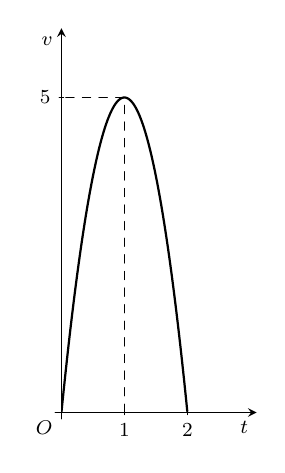
\begin{tikzpicture}[line join=round, line cap=round,>=stealth,font=\footnotesize,scale=0.8]
			\tikzset{every node/.style={scale=0.9}}
			\draw[->] (-0.1,0)--(3.1,0) node[below left] {$t$};
			\draw[->] (0,-0.1)--(0,6.1) node[below left] {$v$};
			\draw (0,0) node [below left] {$O$};
			\foreach \x/\nx in {1/1,2/2}
			\draw[thin] (\x,1pt)--(\x,-1pt) node [below] {$\nx$};
			\foreach \y/\ny in {5/5}
			\draw[thin] (1pt,\y)--(-1pt,\y) node [left] {$\ny$};
			\draw[dashed,thin](1,0)--(1,5)--(0,5);
			\begin{scope}
				\clip (0,0) rectangle (3,6);
				\draw[samples=200,domain=0:2,smooth,thick,variable=\x] plot (\x,{-5*(\x)^2+10*(\x)+0});
			\end{scope}
		\end{tikzpicture}
	\end{center}
	Gia tốc của vật tại thời điểm $t=1{,}5$ (s) bằng
	\shortans{$-5$}
	\loigiai{
		Giả sử đường parabol đi qua gốc tọa độ có dạng $y=at^2+bt$.\\
		Vì parabol đi qua các điểm $(2;0)$ và $(1;5)$ nên ta có hệ
		$$\heva{& 4a+2b=0 \\ & a+b=5}\Leftrightarrow \heva{& a=-5 \\ & b=10.}$$
		Vậy $v(t)=-5t^2+10t$, suy ra $a(t)=v'(t)=-10t+10$.\\
		Tại $t=1{,}5$ (s) thì $a\left(1{,}5\right)=-10\cdot 1{,}5+10=-5$ (m/s$^2$).
	}
\end{bt}

% từ: cau-hoi/lop11/1D9_Xac_suat/1D9-2-3_Quy_tac_cong_cho_hai_bien_co_xung_khac.tex
\begin{ex}%[1D9H2-3]%[ma:34beac35]
 Từ tập  hợp $X=\left\{0;2;3;4;5;8\right\}$. Các khẳng định sau đây, khẳng định nào đúng, khẳng định nào sai?
 \choiceTF 
  {Số các số tự nhiên có bốn  chữ số là $4^6$}
  {Số các số tự nhiên có bốn chữ số đôi một khác nhau là  $\mathrm{A}_6^4$}
  {\True Số các số tự nhiên chẵn có  bốn chữ số đôi một khác nhau là $108$}
  {\True Số các số tự  nhiên chẵn có bốn chữ số đôi một khác nhau và nhỏ hơn $2024$ là $50$}
 \loigiai{ 
  \begin{itemchoice}
   \itemch Gọi số có dạng $\overline{abcd}$.\\ 
   Có $5$ cách chọn cho $a$. Có  $6$ cách chọn cho mỗi vị trí $b$, $c$, $d$.\\
   Theo quy tắc nhân, ta có $5\cdot 6\cdot 6\cdot  6=1080$ số thỏa mãn.
   \itemch  Gọi số có dạng $\overline{abcd}$.\\
   Số các số tự nhiên có bốn chữ số đôi một khác nhau  là $\mathrm{A}_6^4-\mathrm{A}_5^3=300$.
   \itemch Gọi  số có dạng $\overline{abcd}$.
   \begin{itemize}
    \item Nếu $d=0$ thì có $\mathrm{A}_5^3=60$  số thỏa mãn.
    \item Nếu $d\in \left\{2;4;8\right\}$ suy ra có $3$ cách chọn cho $d$, có $4$ cách chọn cho $a$ và có $\mathrm{A}_4^2$ cách chọn $b,c$.\\ 
    Theo quy tắc  nhân, ta có $4\cdot 4\cdot \mathrm{A}_4^2=48$ số thỏa mãn.
   \end{itemize}
   Vậy theo quy  tắc cộng, ta có $60+48=108$ số thỏa mãn.
   \itemch Gọi số  có dạng $\overline{abcd}$.
   \begin{itemize}
    \item Nếu  $a=1$ thì $d$ có $4$ cách chọn và $b,c$ có $\mathrm{A}_4^2$ cách chọn.\\
    Theo quy tắc nhân, ta có $1\cdot 4\cdot 4\cdot 3=48$ số thỏa mãn. 
     \item Nếu $a=2$ thì $\heva{&b=0\\ &c=1}\Rightarrow d\in \left\{4;8\right\}.$\\
    Theo quy tắc  nhân, ta có $1\cdot 1\cdot 1\cdot 2=2$ số thỏa mãn.
   \end{itemize}
   Vậy theo quy tắc cộng, ta có  $48+2=50$ số thỏa mãn.
  \end{itemchoice}
 } 
\end{ex}

% từ: cau-hoi/lop11/1H4_Duong_thang_mat_phang_Quan_he_song_song/1H4-5-1_Cau_hoi_ly_thuyet.tex
\begin{ex}%[1H4N5-1]%[ma:4662d248]
	Phát  biểu nào dưới đây là đúng về phép chiếu song song?
	 \choice
		{\True Phép chiếu  song song biến hai đường thẳng song song thành hai đường thẳng song song hoặc trùng nhau}
		{Phép chiếu song  song biến hai đường thẳng trùng nhau thành hai đường thẳng song song}
		{Phép chiếu song song biến hai đường thẳng bất kỳ thành hai  đường thẳng song song}
		{Phép chiếu  song song biến hai đường thẳng song song thành hai đường thẳng bất kỳ}
	\loigiai{ 
		Phép chiếu song song biến  hai đường thẳng song song thành hai đường thẳng song song hoặc trùng nhau.
	} 
\end{ex}

% từ: cau-hoi/lop12/2D1_Ung_dung_dao_ham_de_khao_sat_ham_so/2D1-1-1_Xet_tinh_don_dieu_cua_ham_so_cho_boi_cong_thu.tex
\begin{bt}%[2D1H1-1]%[ma:eb99c57f]
% nguon: Archive/2024/0. [LVH] BG - 12 New - 4in1-20240625T224301Z-001/0. [LVH] BG - 12 New - 4in1/2. [LVH] TEX SGK 12 NEW-20240418T074833Z-001/2. [LVH] TEX SGK 12 NEW/[LVH] SGK-12-KNTT/data/C1/12-SGK-KNTT-1-3.tex #1101

	Tìm các tiệm cận của đồ thị các hàm số sau:
	\begin{enumerate}[a)]
		\item $y=\dfrac{3-x}{2 x+1}$
		\item $y=\dfrac{2 x^2+x-1}{x+2}$.
	\end{enumerate}
	\loigiai{\begin{enumerate}[a)]
			\item \begin{itemize}
				\item 
				Ta có: $\lim _{x \rightarrow+\infty} f(x)=\lim _{x \rightarrow+\infty} \dfrac{3- x}{2x+1}=\lim _{x \rightarrow+\infty} \dfrac{\dfrac{3}{x}-1}{2+\dfrac{1}{x}}=-\dfrac{1}{2}$. Tương tự, $\lim _{x \rightarrow-\infty} f(x)=-\dfrac{1}{2}$.\\
				Vậy đồ thị hàm số $f(x)$ có tiệm cận ngang là đường thẳng $y=3$.
				\item Ta có: $\lim _{x \rightarrow-\dfrac{1}{2}^{+}} f(x)=\lim _{x \rightarrow-\dfrac{1}{2}^{+}} \dfrac{3-x}{2x+1}=+\infty$. Tương tự, $\lim _{x \rightarrow-\dfrac{1}{2}^{-}} f(x)=-\infty$. Vậy đồ thị hàm số $f(x)$ có tiệm cận đứng là đường thẳng $x=-\dfrac{1}{2}$.
			\end{itemize}
			\item \begin{itemize}
				\item 	Ta có: $\lim _{x \rightarrow+\infty} f(x)=\lim _{x \rightarrow+\infty} \dfrac{2 x^2+x-1}{x+2}=+\infty$. Tương tự, $\lim _{x \rightarrow+\infty} f(x)=\lim _{x \rightarrow-\infty} \dfrac{2 x^2+x-1}{x+2}=-\infty$.\\
				Vậy đồ thị hàm số $f(x)$ không có tiệm cận ngang.
				\item Ta có: $\lim _{x \rightarrow -2^{+}} f(x)=\lim _{x \rightarrow -2^{+}} \dfrac{2 x^2+x-1}{x+2}=+\infty$. Tương tự, $\lim _{x \rightarrow -2^{-}} f(x)=-\infty$.\\
				Vậy đồ thị hàm số $f(x)$ có tiệm cận đứng là đường thẳng $x=-2$.
				\item 	Ta có:
				$$
				\begin{aligned}
					& a=\lim _{x \rightarrow+\infty} \dfrac{f(x)}{x}=\lim _{x \rightarrow+\infty} \dfrac{2 x^2+x-1}{x^2+2x}=2 ; \\
					& b=\lim _{x \rightarrow+\infty}[f(x)-2x]=\lim _{x \rightarrow+\infty} \dfrac{-3 x-1}{x+2}=-3 .
				\end{aligned}
				$$
				(Tương tự, $\lim _{x \rightarrow-\infty} \dfrac{f(x)}{x}=2, \lim _{x \rightarrow-\infty}[f(x)+x]=-3$.)\\
				Vậy đồ thị hàm số $f(x)$ có tiệm cận xiên là đường thẳng $y=2x-3$.
			\end{itemize}
	\end{enumerate}}
\end{bt}

% từ: cau-hoi/lop12/2D1_Ung_dung_dao_ham_de_khao_sat_ham_so/2D1-1-4_Ung_dung_tinh_don_dieu_de_chung_minh_bat_dang.tex
\begin{bt}%[2D1H1-4]%[ma:9b53fe1c]
% nguon: Archive/2024/TaiLieuGiangDay/1.HamSo/1. K12 - 4in1 - Hamso/ThubaiGoc/Bai1-Dang4.tex #2655
[Mức độ 2]%[Dự án bài giảng new 4in1, Trần Quang Thạnh]
	Giải bất phương trình $\log x  > \log (2x-1) + x-1$.
	\loigiai{
	Điều kiện $x>\dfrac{1}{2}$.\\
	Bất phương trình đã cho tương đương với
	$\log x + x > \log(2x-1) +2x-1$.\\
	Vì hàm số $y=f(t)=\log t + t$ có $y'=\dfrac{1}{t\ln10}+1>0$, với mọi $t>0$ nên hàm số $y=f(t)$ đồng biến trên $(0;+\infty)$.\\
	Do đó, từ bất phương trình đã cho ta được
	$$f(x) > f(2x-1) \Leftrightarrow x>2x-1 \Leftrightarrow x<1.$$
	Kết hợp điều kiện, ta có tập nghiệm bất phương trình là $S=\left(\dfrac{1}{2};1\right)$.
	}
\end{bt}

% từ: cau-hoi/lop12/2D1_Ung_dung_dao_ham_de_khao_sat_ham_so/2D1-3-1_GTLN_GTNN_tren_doan.tex
\begin{ex}%[2D1N3-1]%[ma:dc0c3cfd]
	\immini 
	{Cho đồ thị hàm số $y =  f(x)$ có đồ thị như hình vẽ. Khẳng định nào là đúng?
	\choice 
		{Đồ thị hàm số chỉ có 2 đường tiệm cận đứng là các đường  thẳng $x=-1$ và $x=1$}
		{\True Đồ thị  hàm số có 3 đường tiệm cận}
		{Đồ thị hàm số  có 4 đường tiệm cận}
		{Đồ thị hàm số có  2 đường tiệm cận đứng và 1 đường tiệm cận xiên}
		} 
		{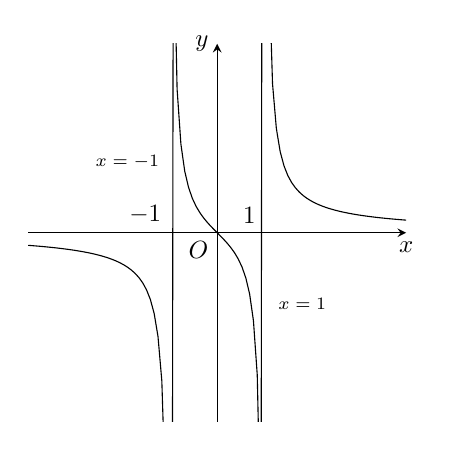
\begin{tikzpicture}[>=stealth,scale=0.6]
		\draw[->]  (-4,0) --(4,0);
		 \draw[->](0,-4)--(0,4);
		\draw (0,0)  node[below left]{$O$};
		 \draw (4,0) node[below]{$x$};
		\draw (0,4) node[left]{$y$}; 
		 \draw (1,0) node[above left]{$1$};
		\draw (-1,0)  node[above left]{$-1$};
		\clip (-4,-4)  rectangle (4,4);
		\draw[samples=100]  plot[domain=-4:4]
			(\x,{(\x)/((\x)^(2)-1)}); 
		\draw (-1.9,1.5) node {\scriptsize $x=-1$}; 
		\draw  (1.8,-1.5) node {\scriptsize $x=1$};
	\end{tikzpicture}
		} 
	\loigiai{Đồ thị hàm số có 2 đường tiệm cận đứng $x=-1$ và $x=1$ và một đường tiệm cận ngang $y=0$, hàm số không có  đường tiệm cận xiên.}
\end{ex}

% từ: cau-hoi/lop12/2D1_Ung_dung_dao_ham_de_khao_sat_ham_so/2D1-3-1_GTLN_GTNN_tren_doan.tex
\begin{ex}%[2D1V3-1]%[ma:5bf782f2]
	Biết rằng đồ thị hàm số $y =  \dfrac{(a - 3)x + a + 2025}{x - (b + 3)}$ nhận trục hoành làm tiệm cận ngang và trục tung làm tiệm cận đứng. Khi đó giá của $a + b$ là
	 \choice
		{$3$} 
		{$-3$} 
		{\True  $0$}
		{$6$} 
	\loigiai{Ta có $\heva{&\lim\limits_{x \to +\infty} \dfrac{(a-3)x + a + 2025}{x-(b+3)} =a-3&\\&\lim\limits_{x \to -\infty}\dfrac{(a-3)x+a+2025}{x-(b+3)}  = a - 3.}$\\
		Mặt khác $\heva{&\lim\limits_{x\to (b+3)^-} \dfrac{(a-3)x+a+2025}{x-(b+3)} = +\infty\\&\lim\limits_{x \to (b+3)^+} \dfrac{(a-3)x+a+2025}{x-(b+3)} = -\infty.}$\\ 
		Suy ra đồ thị hàm số có tiệm cận ngang là đường  thẳng $y=a-3$, tiệm cận đứng là đường thẳng $x=b+3$.\\
		Theo bài ra, ta có $\heva{&a -3 =0 \\&b + 3 = 0} \Rightarrow  \heva{&a = 3\\&b = -3} \Rightarrow a+b=0$.
	} 
\end{ex}

% từ: cau-hoi/lop12/2D1_Ung_dung_dao_ham_de_khao_sat_ham_so/2D1-3-1_GTLN_GTNN_tren_doan.tex
\begin{ex}%[2D1V3-1]%[ma:deec5a80]
	Giao điểm của hai đường tiệm cận của đồ thị hàm  số nào dưới đây nằm trên đường thẳng $d\colon y = x$?
	\choice 
		{$y = \dfrac{2x-1}{x+3}$} 
		{\True$y = \dfrac{x+4}{x-1}$} 
		{$y  = \dfrac{2x+1}{x+2}$}
		{$y =  \dfrac{1}{x+3}$}
	\loigiai{ 
		Đồ thị hàm  số $y = \dfrac{2x-1}{x+3}$ có giao điểm hai đường tiệm cận là $(-3; 2) \notin d$.\\
		Đồ thị hàm số $y = \dfrac{x+4}{x-1}$ có giao điểm hai đường tiệm cận là $(1;  1) \in d$.\\
		Đồ thị hàm số $y = \dfrac{2x+1}{x+2}$ có giao điểm hai đường  tiệm cận là $(-2; 2) \notin d$.\\
		Đồ thị hàm số $y = \dfrac{1}{x+3}$ có giao điểm hai đường tiệm cận là  $(-3; 0) \notin d$.\\
	} 
\end{ex}

% từ: cau-hoi/lop12/2D1_Ung_dung_dao_ham_de_khao_sat_ham_so/2D1-3-1_GTLN_GTNN_tren_doan.tex
\begin{ex}%[2D1H3-1]%[ma:326ac91b]
	\immini 
	{Cho đồ thị của hàm số $f(x)$ như  hình bên.
	 \choiceTF
		{Đường thẳng $y=x+1$ là đường tiệm cận ngang của đồ thị hàm  số $f(x)$}
		 {\True Đồ thị hàm số $f(x)$ có một đường tiệm cận đứng và một đường tiệm cận xiên }
		{\True Hàm số có phương  trình là $f(x)=\dfrac{x^2+2x+2}{x+1}$}
		{\True Đồ thị hàm số $f(x)$  có đường tiệm cận xiên là đường thẳng $y=x+1$}
		 }
		{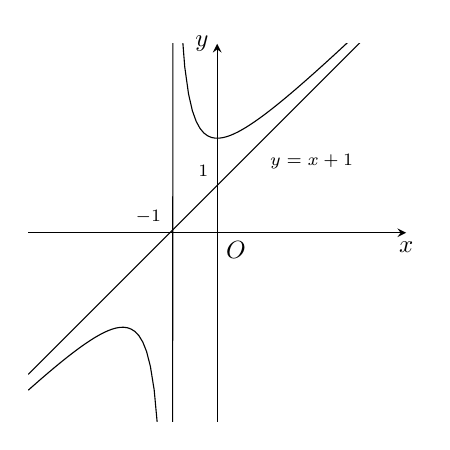
\begin{tikzpicture}[>=stealth,scale=0.6]
		\draw[->] (-4,0) --(4,0); 
		 \draw[->](0,-4)--(0,4);
		\draw (0,0)  node[below right]{$O$};
		\draw  (4,0) node[below]{$x$};
		\draw (0,4) node[left]{$y$}; 
		\draw  (-1,0) node[above left]{\scriptsize $-1$};
		\draw (0,1) node[above left]{\scriptsize $1$}; 
		\clip (-4,-4) rectangle  (4,4);
		\draw[samples=100] plot[domain=-4:4] 
			(\x,{((\x)^2+2*\x+2)/((\x)+1)}); 
		\draw[samples=100] plot[domain=-4:4] 
			 (\x,{\x+1});
		\draw (2,1.5)  node {\scriptsize $y=x+1$};
	\end{tikzpicture}
		} 
	 \loigiai{
		\begin{itemchoice}
			\itemch Dựa vào đồ thị hàm số của $f(x)$, đồ thị hàm số không có tiệm cận  ngang.
			\itemch Dựa vào đồ thị hàm số của $f(x)$, đồ thị hàm  số có đường tiệm cận đứng $x=-1$.
			\itemch Gọi $y=ax+b,a\neq0$ là phương trình đường tiệm  cận xiên của đồ thị hàm số $f(x)$.\\
			$a = \lim\limits_{x \to +\infty} \dfrac{f(x)}{x} = \lim\limits_{x \to +\infty} \dfrac{\dfrac{x^2+2x+2}{x+1}}{x} = \lim\limits_{x  \to +\infty} \dfrac{x^2+2x+2}{x(x+1)} = 1$.\\
			$b = \lim\limits_{x  \to +\infty}[f(x)-ax] = \lim\limits_{x \to +\infty} \left[\dfrac{x^2 + 2x + 2}{x + 1} - x\right]=1$.\\
			Vậy đường thẳng $y=x+1$ là  đường tiệm cận xiên của đồ thị hàm số $f(x)$.\\
			Ta có  $\heva{&\lim\limits_{x \to -1^+} \dfrac{x^2+2x+2}{x+1} = +\infty\\&
			\lim\limits_{x \to  -1^-} \dfrac{x^2+2x+2}{x+1}= -\infty.}$\\
			Vậy $x=-1$  là phương trình đường tiệm cận đứng.
			\itemch  Dựa vào đồ thị, đường thẳng $y=x+1$ là đường tiệm cận xiên của đồ thị hàm số $f(x)$.
		\end{itemchoice}
	 }
\end{ex}

% từ: cau-hoi/lop12/2D1_Ung_dung_dao_ham_de_khao_sat_ham_so/2D1-3-1_GTLN_GTNN_tren_doan.tex
\begin{bt}%[2D1V3-1]%[ma:88d3ebe3]
	Cho hàm  số $f(x)$ xác định và liên tục trên $\mathbb{R}\setminus\{-1\}$, có bảng biến thiên như sau:
	\begin{center}
		
\begin{tikzpicture}
			 \tkzTabInit[lgt=1.5,espcl=3,deltacl=.5]
				{$x$/0.7,$f’(x)$/0.7,$f (x)$/2} 
				{$-\infty$,$-1$,$+\infty$} 
			 \tkzTabLine{,-,d,-,}
			\tkzTabVar{+/$2$,-D+/$-\infty$/$+\infty$,-/$-2$} 
		\end{tikzpicture}
	\end{center}
	Hỏi đồ thị hàm số $y=\dfrac{1}{f(x)}$ có  tất cả bao nhiêu đường tiệm cận đứng và tiệm cận ngang?
	 \shortans{4}
	 \loigiai{Dựa vào bảng biến thiên ta có
		$$\lim\limits_{x\to  -\infty}f(x)=2, \lim\limits_{x\to +\infty} f(x) = -2, \lim\limits_{x\to -1^-} f(x) = -\infty, \lim\limits_{x\to -1^+} f(x) = +\infty.$$
		Đặt $y=g(x)=\dfrac{1}{f(x)}$. Ta  có $\lim\limits_{x\to +\infty}g(x) = \lim\limits_{x \to +\infty} \dfrac{1}{f(x)} = \dfrac{-1}{2} \Rightarrow$ đường thẳng $y = -\dfrac{1}{2}$ là tiệm cận ngang của đồ thị hàm số $y=g(x)=\dfrac{1}{f(x)}$.\\
		Vì $\lim\limits_{x\to -\infty} g(x) = \lim\limits_{x \to -\infty} \dfrac{1}{f(x)} = \dfrac{1}{2}\Rightarrow$ đường thẳng  $y = \dfrac{1}{2}$ là tiệm cận ngang của đồ thị hàm số $y=g(x)=\dfrac{1}{f(x)}$.\\
		Mặt khác  $\lim\limits_{x \to -1} g(x) = \lim\limits_{x \to -1} \dfrac{1}{f(x)} = 0 \Rightarrow$ đường thẳng $x=-1$ không là tiệm cận đứng của đồ thị hàm số $y = g(x) = \dfrac{1}{f(x)}$.\\
		Xét phương trình $f(x)=0$, ta  có
		\begin{center}
			\begin{tikzpicture}
				 \tkzTabInit[lgt=1.5,espcl=3,deltacl=.5]
					 {$x$/0.7,$f’(x)$/0.7,$f (x)$/2}
					{$-\infty$,$-1$,$+\infty$} 
				 \tkzTabLine{,+,d,-,}
				 \tkzTabVar{+/$2$,-D+/$-\infty$/$+\infty$,-/$-2$}
				\draw[red] (2,-2.3)--(8,-2.3) node[above]{$y=0$}; 
			\end{tikzpicture}
		\end{center}
		Dựa vào BBT ta thấy phương trình  có hai nghiệm phân biệt thỏa mãn khác $-1$.\\
		 Do đó đồ thị hàm số $y=g(x)=\dfrac{1}{f(x)}$ có $2$ tiệm cận đứng.\\
		Vậy  đồ thị hàm số $y=g(x)=\dfrac{1}{f(x)}$ có tất cả $4$ đường tiệm cận.
	} 
\end{bt}

% từ: cau-hoi/lop12/2D1_Ung_dung_dao_ham_de_khao_sat_ham_so/2D1-4-1_Bai_toan_xac_dinh_cac_duong_tiem_can_cua_ham.tex
\begin{ex}%[2D1N4-1]%[ma:3c351e5e]
	\immini{Cho hàm số $f(x)$ có đồ thị như hình bên. Biết rằng  một trong bốn điểm sau đây là tâm đối xứng của đồ thị hàm số, điểm đó là điểm nào?
	 \choice
		 {$M(0;1)$}
		{\True  $N(-1;2)$}
		{$P(-2;3)$} 
		 {$Q(0;3)$}
		}{\resizebox{!}{5cm}{\begin{tikzpicture}[line join=round,line cap=round,>=stealth]
		 \tikzset{label style/.style={font=\footnotesize}}
		 \draw[->] (-4.1,0)--(3.1,0) node[below left] {$x$};
		\draw[->] (0,-2.1)--(0,5.1) node[below  left] {$y$};
		\draw (0,0)  node [below left] {$O$};
		\foreach \x  in {-3,-2,-1,1,2}
		\draw (\x,1pt)--(\x,-1pt) node [below]  {$\x$};
		\foreach  \y in {-2,-1,1,2,3,4}
		\draw (1pt,\y)--(-1pt,\y) node [left] {$\y$}; 
		\begin{scope}
			\clip  (-4,-2) rectangle (3,5);
			\draw[samples=100,domain=-4:-1.01,smooth,variable=\x] plot  (\x,{(2*(\x)+1)/((\x)+1)});
			 \draw[samples=100,domain=-0.99:3,smooth,variable=\x] plot (\x,{(2*(\x)+1)/((\x)+1)});
		\end{scope}
	\end{tikzpicture}
		 }}
	\loigiai{Đồ thị hàm số có tiệm cận đứng $x=-1$, và tiệm cận ngang là  $y=2$ nên tâm đối xứng là $N\left(-1;2\right)$.}
\end{ex}

% từ: cau-hoi/lop12/2D1_Ung_dung_dao_ham_de_khao_sat_ham_so/2D1-5-1_Nhan_dang_do_thi.tex
\begin{ex}%[2D1H5-1]%[ma:43d9abff]
	Cho hàm  số $y=\dfrac{mx-1}{2x+m}$ có đồ thị là $\left(C_m \right)$ với $m$ là tham số
	\choiceTF 
		{\True Khi $m=2$ thì đồ thị hàm số  có đường tiệm cận ngang $y=1$}
		{Khi $m=2$  thì giao điểm của các đường tiệm cận có toạ độ $I\left(1;-1\right)$}
		{\True Đường tiệm cận đứng của đồ  thị hàm số đi qua điểm $A\left(-1; \sqrt{2} \right)$ thì $m=2$}
		{\True Với mọi giá trị của tham số $m$ thì hàm số luôn đồng biến trên mỗi khoảng  xác định của nó}
	\loigiai{ 
		\begin{itemchoice}
			 \itemch
			Khi $m=2$ thì đồ thị  hàm số có đường tiệm cận ngang $y=1$.
			\itemch 
			Khi $m=2$ thì giao điểm của các đường  tiệm cận có toạ độ $I\left(-1; 1\right)$.
			 \itemch
			Đồ thị hàm số có tiệm cận đứng khi và chỉ khi $m\left(-\dfrac{m}{2} \right)-1\ne 0\Leftrightarrow m^2+2\ne 0$  đúng với mọi giá trị $m$.\\
			Khi đó, TCĐ là đường thẳng $x=-\dfrac{m}{2}$. Vì TCĐ đi qua điểm $A(-1; \sqrt{2})$ nên ta có $-\dfrac{m}{2}=-1\Leftrightarrow m=2$. 
			 \itemch
			Ta có $y'=\dfrac{m^2+2}{\left(2x+m\right)^2}  > 0, \forall x\ne-\dfrac{m}{2}$.\\
			Vậy hàm số đồng biến trên từng khoảng xác định  của nó.
		\end{itemchoice}
	} 
\end{ex}

% từ: cau-hoi/lop12/2D1_Ung_dung_dao_ham_de_khao_sat_ham_so/2D1-5-2_Cac_phep_bien_doi_do_thi.tex
\begin{bt}%[2D1H5-2]%[ma:05edb71f]
% nguon: Archive/2024/TaiLieuGiangDay/1.HamSo/1. K12 - 4in1 - Hamso/ThubaiGoc/Bai5-Dang4.tex #2235
[Mức độ 2]%[Bài giảng 12 mới, Lê Hồng Phi]
Tìm phương trình đường tiệm cận đứng của đồ thị hàm số $y=\log_2 (x-3)$.
\loigiai
{Đồ thị hàm số $y=f(x)=\log_2 x$ có tiệm cận đứng là $x=0$.\\
Đồ thị hàm số $y=\log_2(x-3)=f(x-3)$ có được bằng cách tịnh tiến đồ thị hàm số $y=\log_2 x$ sang phải $3$ đơn vị nên có phương trình đường tiệm cận đứng là $x=3$.
}
\end{bt}

% từ: cau-hoi/lop12/2D1_Ung_dung_dao_ham_de_khao_sat_ham_so/2D1-5-6_Phuong_trinh_tiep_tuyen_cua_do_thi_ham_so.tex
\begin{ex}%[2D1N5-6]%[ma:2806087a]
	Đạo hàm của hàm số $y= f(x)$ tại điểm $x_0$ là hệ số góc của tiếp tuyến với đồ thị $(C)$ của hàm số tại điểm $M_0(x_0; f(x_0))$. Khi đó phương trình tiếp tuyến của $(C)$ tại điểm $M_0$  là
	\choice 
		{$y+y_0=f'(x_0)\cdot  (x-x_0)$}
		{$y-y_0=f'(x_0)\cdot  (x+x_0)$}
		{\True $y-y_0=f'(x_0)\cdot  (x-x_0)$}
		{$y-y_0=f'(x_0)\cdot  (x_0-x)$}
	\loigiai{ 
	 }
\end{ex}

% từ: cau-hoi/lop12/2D4_Nguyen_ham_tich_phan/2D4-1-3_Nguyen_ham_co_ban_ham_luong_giac.tex
\begin{ex}%[2D4H1-3]%[ma:2f9ec564]
	Chiều cao của các bạn học sinh nữ lớp $12\mathrm{B}$ được ghi  lại ở bảng sau
	\begin{center}
		\begin{tabular}{|m{3.5cm}|m{2.5 cm}|m{2.5 cm}|m{2.5 cm}|m{2.5 cm}|}
			 \hline
			\centering\arraybackslash  Chiều cao $(\mathrm{cm})$&
			 \centering\arraybackslash$[155;160)$&
			\centering\arraybackslash$[160;165)$& 
			\centering\arraybackslash$[165;170)$& 
			\centering\arraybackslash$[170;175)$\\ 
			\hline 
			\centering\arraybackslash Số học  sinh&
			 \centering\arraybackslash$2$&
			\centering\arraybackslash$5$& 
			 \centering\arraybackslash$8$&
			\centering\arraybackslash$5$\\ 
			 \hline
		\end{tabular}
	\end{center}
	Khoảng  tứ phân vị của mẫu số liệu ghép nhóm trên là
	 \choice
		{$5$} 
		 {$6$}
		 {\True $7$}
		 {$8$}
	 \loigiai{
		Cỡ mẫu  $n=20$.\\
		Gọi $x_1,; x_2;\ldots;x_{20}$ là mẫu số liệu gốc gồm chiều cao của các bạn học sinh nữ được sắp xếp theo  thứ tự không giảm.\\
		 Tứ phân vị thứ nhất của mẫu số liệu gốc là $Q_1=\dfrac{1}{2}(x_{5}+x_{6})\in [160;165)$.\\
		Do đó  tứ phân vị thứ nhất của mẫu số liệu ghép nhóm là $$Q_1=160+\dfrac{\dfrac{20}{4}-2}{5}\cdot(165-160)=163\mathrm{\,(cm)}.$$
		Tứ  phân vị thứ ba của mẫu số liệu gốc là $Q_3=\dfrac{1}{2}(x_{15}+x_{16})$.\\
		Mà  $x_{15}\in [165;170)$ và $x_{16}\in [170;175)$.\\
		Do đó tứ phân vị thứ ba của mẫu số liệu ghép  nhóm là $Q_3=170$.\\
		Khoảng  tứ phân vị $\Delta Q=Q_3-Q_1=170-163=7\mathrm{\,(cm)}$.
	 }
\end{ex}

% từ: cau-hoi/lop12/2D4_Nguyen_ham_tich_phan/2D4-1-6_Toan_thuc_te_ap_dung_nguyen_ham.tex
\begin{bt}%[2D4V1-6]%[ma:9a62a10a]
% nguon: Archive/2024/San pham - To Latex Strong - Tex hoa Lop 12 moi - Dot 3 (Chuong 1 + 2 +3 + 4)/Data/Chuong 4/Canh dieu/To 19 - Dot 17 - Chuong 4 - Bai 2 - CD - De 1.tex #3445
%
 \immini{Một vật chuyển động trong $4$ giờ với vận tốc $v$ (km / h) phụ thuộc vào thời gian $t$ (h) có đồ thị vận tốc là một đường parabol có đỉnh $I(3 ; 10)$ và trục đối xứng vuông góc với trục hoành như hình vẽ. Tính quãng đường vật di chuyển được trong nửa thời gian sau của chuyển động đó (kết quả làm tròn đến hàng phần chục và tính theo đơn vị km )}
 {
 	\begin{tikzpicture}[scale=0.4,>=stealth, font=\footnotesize, line join=round, line cap=round]
 	\def\xmin{-3} \def\xmax{6}
 	\def\ymin{-1} \def\ymax{11}
 	\draw[->] (\xmin,0)--(\xmax,0) node [below]{$t$};
 	\draw[->] (0,\ymin)--(0,\ymax) node [left]{$v$};
 	\fill (0,0) circle (1pt) node[shift={(-135:2.5mm)}]{$O$};
 	\clip (\xmin+0.1,\ymin+0.1) rectangle (\xmax-0.1,\ymax-0.1);
 	\draw[smooth,red,samples=300,domain=(0:4)] plot(\x,{-(\x)^2+6*(\x)+1});	
 	\foreach \x in {\xmin,...,\xmax}
 	\draw (\x,-0.05)--(\x,0.05);
 	\foreach \y in {\ymin,...,\ymax}
 	\draw (-0.05,\y)--(0.05,\y);	
 	\node at (3,0)[below]{$3$};
 	\node at (0,1)[left]{$1$};
 	\node at (0,10)[left]{$10$};
 	\draw[dashed] (0,10)--(3,10)--(3,0);
 	%\node at (-1,1)[shift={(70:2mm)}]{$ I $};
 	%\draw[dashed]
 	%(-1,0)node[below]{$ -1 $}|-(0,1)node[right]{$1$}	
 %	;	
 \end{tikzpicture}
 }
\shortans{$19{,}3$}

\loigiai{
Dựa vào đồ thị ta tìm được vận tốc $v(t)=-t^{2}+6 t+1, t \in[0 ; 4]$.\\
Quãng đường $s(t)$ vật di chuyển được trong thời gian $4$h là một nguyên hàm của $v(t)$, với $t \in[0 ; 4]$\\
Ta có $s(t)=\displaystyle\int\left(-t^{2}+6t+1\right) \mathrm{d}t=-\dfrac{t^{3}}{3}+3 t^{2}+t+C$.\\
Quãng đường vật di chuyển được trong $2$h đầu là $s(2)=\dfrac{34}{3}+C$ (km).\\
Quãng đường vật di chuyển được trong $4$h là $s(4)=\dfrac{92}{3}+C$ (km).\\
Quãng đường vật di chuyển được trong nửa thời gian sau của chuyển động là
$$s(4)-s(2)=\dfrac{58}{3} \text{~(km)} \approx 19{,}3\text{~(km)}.$$}

\end{bt}

% từ: cau-hoi/lop12/2D4_Nguyen_ham_tich_phan/2D4-2-2_Tich_phan_co_ban_da_thuc_phan_thuc.tex
\begin{bt}%[2D4N2-2]%[ma:753ee6dd]
% nguon: Archive/SP-4Phan-Dot3/Data/CD_2-OTGK2-De04.tex #4440
%[Dự án đề 4 phần]%[Đoàn Hùng]
	Tính diện tích hình phẳng giới hạn bởi đồ thị hàm số $y=\ln x$, trục $Ox$ và đường thẳng $x=\mathrm{e}$.
	\loigiai{
		Ta có $\ln x=0\Leftrightarrow x=1$. Vậy $S=\displaystyle\int\limits_0^{\mathrm{e}}|\ln x|\mathrm{\,d}x=1$.}
\end{bt}

% từ: cau-hoi/lop12/2D4_Nguyen_ham_tich_phan/2D4-2-6_Toan_thuc_te_ap_dung_nguyen_ham.tex
\begin{bt}%[2D4V2-6]%[ma:767b5e58]
	 \immini
	{Cho parabol $\left(P_1\right) \colon y = -x^2 + 6$ cắt trục hoành tại hai điểm phân biệt $A$ và $B$; parabol $\left(P_2\right)$ đi qua hai điểm $A$; $B$ và có đỉnh nằm trên đường thẳng $d \colon y = a$, $(0 < a <6)$. Gọi $S_1$ là diện tích hình phẳng giới hạn bởi $\left(P_1\right)$ và $d$; gọi $S_2$ là diện tích hình phẳng giới hạn bởi $\left(P_2\right)$  và trục hoành (tham khảo hình vẽ). Biết rằng $S_1 = S_2$. Tính giá trị của biểu thức $T = a^3 - 12a^2 + 108a$.
	} 
	{\begin{tikzpicture}[>=stealth,line join=round,line cap=round,color=blue,font=\footnotesize,scale=0.7]
		\draw[->] (-4,0) -- (4,0) node[below] {$x$}; 
		\draw[->] (0,-1)--(0,6.5)  node[right]{$y$};
		 \draw (0,0) node[below left]{$O$};
		\draw (-2.45,0) node[above  left]{\scriptsize $-\sqrt{6}$}
			(-2.45,0)  node[below right]{\scriptsize $A$}
			(2.45,0) node[above right]{\scriptsize $\sqrt{6}$} 
			(2.45,0)  node[below left]{\scriptsize $B$};
		\fill[pattern = north east lines,pattern color=cyan,smooth] plot[domain=-1.85:1.85] (\x,{-(\x)^2+6})--(1.85,2.58)--(-1.85,2.58)--cycle; 
		 \fill[pattern = north west lines,pattern color=red,smooth] plot[domain=-1.85:1.85] (\x,{0.43*(-(\x)^2+6)})--(2.45,0)--(-2.45,0)--cycle;
		\draw[violet,samples=150,smooth,domain=-2.55:2.55] plot  (\x,{-(\x)^2+6});
		\draw[violet,samples=150,smooth,domain=-2.7:2.7] plot (\x,{0.43*(-(\x)^2+6)}); 
		\draw (-4,2.58)--(4,2.58); 
		 \draw (3.2,2.6) node[above]{\scriptsize $y = a$};
		\draw (1.6,4.5) node[above]{\scriptsize $(P_1)$}; 
		 \draw (1.5,1.8) node[above]{\scriptsize $(P_2)$};
	\end{tikzpicture}
	 }
	\shortans{216} 
	 \loigiai{
		Hoành độ giao điểm của  $\left(P_1\right)$ và $d$ là nghiệm của phương trình $a = -x^2 + 6 \Rightarrow x = \pm \sqrt{6-a}$.\\
		Ta có $\left(P_2\right)$ cắt  trục hoành tại hai điểm có hoành độ $\pm \sqrt{6}$ nên có dạng $y = k\left(-x^2 + 6\right)$.\\
		Do $\left(P_2\right)$ đi qua điểm $(0; a)$ nên $a = k\left(-0^2 + 6\right)  \Rightarrow k = \dfrac{a}{6}$.\\
		Vậy $\left(P_2\right) \colon y = \dfrac{a}{6} \left(-x^2  + 6\right)$.\\
		Khi đó ta có $$S_1 = \displaystyle\int_{-\sqrt{6-a}}^{\sqrt{6-a}} \left(6-x^2-a\right) \mathrm{\,d}x = \dfrac{4}{3} \sqrt{6-a} \cdot(6-a);$$ $$S_2 = \displaystyle\int_{-\sqrt{6}}^{\sqrt{6}} \dfrac{a}{6}  \left(-x^2 + 6\right) \mathrm{\,d}x = \dfrac{4\sqrt{6}}{3}a.$$
		 Do $S_1 = S_2$ nên ta có
		 {\allowdisplaybreaks
		\begin{eqnarray*}
			\dfrac{4}{3} \sqrt{6 - a} \cdot (6 - a) =  \dfrac{4\sqrt{6}}{3}a
			&\Leftrightarrow& \sqrt{6 - a} \cdot (6 - a) =  \sqrt{6}a\\
			&\Leftrightarrow& a^3 - 12a^2 + 108a= 216\\ 
			&\Rightarrow&  T = 216.
		\end{eqnarray*}
		} 
	} 
\end{bt}

% từ: cau-hoi/lop12/2D4_Nguyen_ham_tich_phan/2D4-2-6_Toan_thuc_te_ap_dung_nguyen_ham.tex
\begin{bt}%[2D4H2-6]%[ma:18b2835f]
	Xét chiếc chén trong một bộ ấm chén uống trà, bạn Dương ước lượng được  rằng chiếc chén được tạo thành khi cho hình phẳng giới hạn bởi đồ thị hàm số $f(x)=0{,}14x^3-0{,}87x^2+1{,}92x+0{,}85$, trục hoành và hai đường thẳng $x=0$, $x=3$ quay quanh trục $Ox$ (đơn vị trên mỗi trục toạ độ là centimét). Tính thể tích của chiếc chén (làm tròn đến hàng đơn vị của centimét khối).
	\begin{center}
		\resizebox{!}{5cm}{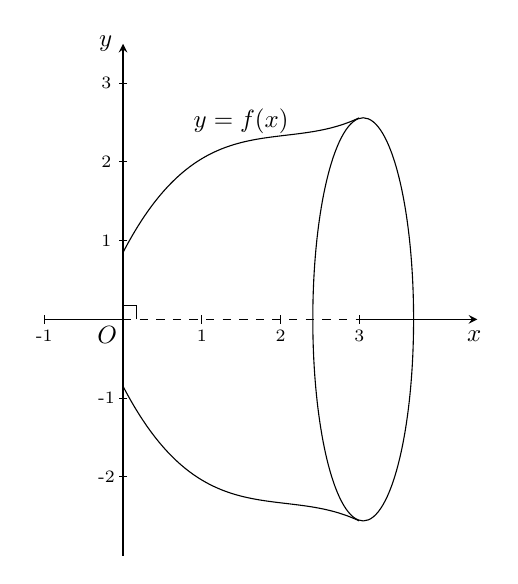
\begin{tikzpicture}[line cap=butt,line join=miter,>=stealth]
		\draw[->]  (-1,0)--(0,0)
			(3,0)--(4.5,0) 
			node[shift={(-100:7pt)},font=\normalsize]{$x$}; 
		 \draw[->] (0,-3)--(0,3.5)
			node[shift={(180:7pt)},font=\normalsize]{$y$}; 
		\draw[dashed] (0,0)--(3,0); 
		\draw (5pt,0) |-  (0,5pt)
			(0,0) node[shift={(225:9pt)},font=\normalsize]{$O$}; 
		\foreach \x in {-1,1,2,3}{ 
			 \draw (\x,1.5pt)--(\x,-1.5pt) node[font=\scriptsize,shift={(-90:5pt)}]{\x};
		} 
		\foreach \y in  {-2,-1,1,2,3}{
			 \draw (1.5pt,\y)--(-1.5pt,\y) node[font=\scriptsize,shift={(180:5pt)}]{\y};
		 }
		\tikzset{declare function={f  (\x)=(14/100)*(\x)^3-(87/100)*(\x)^2+(192/100)*(\x)+85/100; a=f (3);}}
		 \draw[samples=100] plot[domain=0:3] (\x,{f (\x)});
		\draw[samples=100] plot[domain=0:3] (\x,{-f  (\x)});
		\draw (3.05,0) ellipse ({0.25*a} and  a);
		 \path (1.5,{f (1.5)}) node[above]{$y=f (x)$};
	\end{tikzpicture}}
	\end{center}
	\loigiai{ 
		Thể tích của chiếc chén  là: $V=\pi\displaystyle\int_0^3\left(0{,}14x^3-0{,}87x^2+1{,}92x+0{,}85\right)^2\mathrm{d}x=41{,}87\,(\mathrm{cm}^3)$.
	 }
\end{bt}

% từ: cau-hoi/lop12/2D4_Nguyen_ham_tich_phan/2D4-2-6_Toan_thuc_te_ap_dung_nguyen_ham.tex
\begin{bt}%[2D4V2-6]%[ma:591c1ebe]
	Cho hình phẳng $(H)$ được giới hạn bởi đường cong $y=\sqrt{m^2-x^2}$ ($m$ là tham số khác $0$) và trục hoành. Khi $(H)$ quay xung quanh trục hoành được khối tròn xoay có thể tích $V$. Có bao nhiêu giá trị nguyên của $m$ để $V< 1\,000\pi$. 
	 \loigiai{
		Phương trình hoành độ giao điểm  của đường cong và trục hoành là: $\sqrt{m^2-x^2}=0\Leftrightarrow x=\pm m$.\\
		Thể tích vật thể tròn xoay cần tính là: $V=\pi \displaystyle\int_{-\left|m\right|}^{\left|m\right|}\left(m^2-x^2\right)\mathrm{d}x=\pi \left(m^2x-\dfrac{1}{3} x^3\right)\left|\begin{array}{l} |m|\\-|m|
	\end{array}\right.=\dfrac{4\pi m^2\left|m\right|}{3}$.\\
	Ta có: $V< 1\,000\pi$ $\Leftrightarrow \dfrac{4\pi m^2\left|m\right|}{3} < 1\,000\pi$ $\Leftrightarrow \left|m\right|^3< 750$ $\Leftrightarrow-\sqrt[3]{750} <  m < \sqrt[3]{750}$.\\
	 Ta có $\sqrt[3]{750} \simeq 9{,}08$ và $m\ne 0$.\\
	Suy ra, các giá  trị $m$ nguyên là $m\in \left\{-9;-8;-7;-6;-5;-4;-3;-2;-1;1;2;3;4;5;6;7;8;9\right\}$.\\
	Vậy có $18$ giá trị nguyên  của $m$.
 }
\end{bt}

% từ: cau-hoi/lop12/2H2_Toa_do_cua_vec_to_trong_khong_gian/2H2-2-4_Cong_thuc_toa_do_cua_tich_vo_huong_va_ung_dun.tex
\begin{ex}%[2H2N2-4]%[ma:fd25a3aa]
	Trong không gian $Oxyz$,  cho hai đường thẳng $d_{1}\colon \dfrac{x}{-1}=\dfrac{y+1}{1}=\dfrac{z-9}{-2}$,\break$d_{2}\colon \dfrac{x+1}{-1}=\dfrac{y-1}{1}=\dfrac{z+5}{1}$. Góc giữa hai đường thẳng $d_1$ và $d_2$ bằng
	 \choice
		{\True  $90^{\circ}$}
		 {$60^{\circ}$}
		{$45^{\circ}$} 
		 {$30^{\circ}$}
	 \loigiai{
		Đường thẳng  $d_{1}$, $d_{2}$ có vectơ chỉ phương lần lượt là $\overrightarrow{u}_1=(-1;1;-2)$, $\overrightarrow{u}_2=(-1;1;1)$.\\
		Ta có 
		$$ 
		\cos (d_{1},d_{2})=\dfrac{\left|\overrightarrow{u}_1\cdot \overrightarrow{u}_2\right|}{|\overrightarrow{u}_1|\cdot|\overrightarrow{u}_2|} 
		 =\dfrac{|(-1)\cdot(-1)+1\cdot1+(-2)\cdot1|}{\sqrt{(-1)^{2}+1^{2}+(-2)^{2}}\cdot \sqrt{(-1)^{2}+1^{2}+1^{2}}}
		=\dfrac{|1+1-2|}{\sqrt{6}\cdot  \sqrt{3}}=0.
		$$ 
		Do đó góc giữa hai  đường thẳng đã cho là $90^{\circ}$.
	} 
\end{ex}

% từ: cau-hoi/lop12/2H2_Toa_do_cua_vec_to_trong_khong_gian/2H2-2-4_Cong_thuc_toa_do_cua_tich_vo_huong_va_ung_dun.tex
\begin{ex}%[2H2H2-4]%[ma:aa909a49]
	Cho tam giác $ABC$ có $A\left(1;2;0\right)$,  $B\left(0;1;1\right)$, $C\left(2;1;0\right)$.
	 \choiceTF
		{\True Tam giác $ABC$  vuông tại $A$}
		{Chu  vi tam giác là $\sqrt{7}+\sqrt{3}+\sqrt{2}$}
		{Diện tích tam giác $ABC$ là  $\sqrt{6}$}
		{\True Tâm đường tròn ngoại  tiếp tam giác $ABC$ là $I\left(1;1;\dfrac{1}{2} \right)$}
	 \loigiai{
		Ta có $\overrightarrow{AB}=\left(-1;-1;1\right)\Rightarrow AB=\sqrt{3}$, $\overrightarrow{AC}=\left(1;-1;0\right)\Rightarrow AC=\sqrt{2}$,\\ $\overrightarrow{BC}=\left(2;0;-1\right)\Rightarrow  BC=\sqrt{5}$.
		\begin{itemchoice}
			\itemch $\overrightarrow{AB}\cdot \overrightarrow{AC}=0$  do đó $AB\perp AC$, tam giác $ABC$ vuông tại $A$.
			\itemch Chu vi của tam giác  là $AB+AC+BC=\sqrt{3}+\sqrt{2}+\sqrt{5}$.
			\itemch Diện tích $\triangle ABC$ là $S=\dfrac{1}{2} \cdot  AB\cdot AC=\dfrac{\sqrt{6}}{2}$
			\itemch Tâm  đường tròn ngoại tiếp là trung điểm của $BC$ có tọa độ $I\left(1;1;\dfrac{1}{2} \right)$.
		\end{itemchoice}
	} 
\end{ex}

% từ: cau-hoi/lop12/2H5_Phuong_trinh_mat_phang_duong_thang_mat_c/2H5-1-6_Goc_giua_hai_mat_phang.tex
\begin{bt}%[2H5H1-6]%[ma:b109c143]
	Cho hình chóp $S.ABCD$ có đáy $ABCD$ là hình vuông cạnh có cạnh bằng $a$ và  $SA \perp (ABCD)$. Khi $a = 2$, hãy tính độ dài cạnh $SA$ để góc tạo bởi $(SBC)$ và $(SDC)$ bằng $60^\circ$.
	\shortans{2} 
	\loigiai{ 
		Chọn  hệ trục như hình vẽ dưới đây.\\
		Gọi $M$  là trung điểm của $SC$.\\
		Đặt $SA=2m$,  $m>0$.
		\begin{center}
			\begin{tikzpicture}[scale=0.65,font=\footnotesize,>=stealth]
					 \path
						(0,0) coordinate (D) 
						(-3,-2) coordinate (A) 
						(5,0)  coordinate (C)
						($(A)+(C)-(D)$)  coordinate (B)
						($(D)!0.5!(B)$)  coordinate (O)
						($(A)+(0,6)$) coordinate (S) 
						($(O)+(0,3)$) coordinate (M); 
					\draw[->] (C)--(7,0.5)  node[below]{$y$};
					 \draw[->] (B)--(3,-3) node[below]{$x$};
					\draw[->] (M)--(1,4.5) node[left]{$z$}; 
					\draw  (B)--(C)--(S)--(B)--(A)--(S);
					 \draw[dashed] (S)--(D)--(C)--(A)--(D)--(B)
						(M)--(O); 
					\foreach \x/\g  in {C/90,D/180,A/-100,B/-90,S/90,M/30,O/-90}\draw (\x) circle (.04) +(\g:.6) node{\footnotesize$\x$};
				\end{tikzpicture}
		\end{center}
		Khi đó $B\left(  \dfrac{a}{\sqrt{2}}; 0; 0 \right),\
		D\left( -\dfrac{a}{\sqrt{2}};  0; 0 \right),\
		C\left( 0;  \dfrac{a}{\sqrt{2}}; 0 \right),\
		M(0;0;m),\  S(0;0;2m).$\\
		Ta có $ 
		 \overrightarrow{n}_{SBC} = \left( 1;1;\dfrac{a}{m\sqrt{2}} \right),\quad
		 \overrightarrow{n}_{SDC} = \left( -1;1;\dfrac{a}{m\sqrt{2}} \right).$\\
		Yêu cầu bài toán $\cos \theta = \dfrac{1}{2}$, với $\theta = \widehat{(SBC),(SDC)}$.\\ 
		Áp dụng công thức  tích vô hướng
		$$ 
		\cos\theta  = \dfrac{|\overrightarrow{n}_1 \cdot \overrightarrow{n}_2|}{|\overrightarrow{n}_1|\cdot\|\overrightarrow{n}_2\|}
		= \dfrac{| -1 +  1 + \left(\dfrac{a}{m\sqrt{2}}\right)^2 |}
		{1 + 1 + \left( \dfrac{a}{m\sqrt{2}}  \right)^2} = \dfrac{1}{2}
		\Rightarrow \left( \dfrac{a}{m\sqrt{2}} \right)^2 = 1 
		\Rightarrow \dfrac{a}{m\sqrt{2}}  = \pm 1.
		 $$
		Với $a = 2 \Rightarrow  m = \sqrt{2} \Rightarrow SA = 2m = 2$.
	} 
\end{bt}

% từ: cau-hoi/lop12/2H5_Phuong_trinh_mat_phang_duong_thang_mat_c/2H5-2-4_Vi_tri_tuong_doi_giua_hai_duong_thang.tex
\begin{ex}%[2H5V2-4]%[ma:8723cef8]
	Cho hình chóp $S.ABCD$ có đáy $ABCD$ là hình vuông cạnh bằng $10$. Cạnh bên $SA$ vuông góc với mặt phẳng $(ABCD)$ và $SC = 10\sqrt{5}$. Gọi $M, N$ lần lượt là trung  điểm của $SA$ và $CD$. Tính khoảng cách $d$ giữa $BD$ và $MN$.
	\loigiai{ 
		Xét tam giác  vuông $SAC$ có
		 $$
		 SA = \sqrt{SC^2 - AC^2} = \sqrt{500 - 200} = 10\sqrt{3}.
		$$ 
		Chọn hệ trục  tọa độ như hình vẽ sao cho\\
		$ 
		A(0;0;0)$, $ B(10;0;0)$,  $ D(0;10;0)$, $ C(10;10;0)$, $ S\left(0;0;10\sqrt{3}\right)$, $
		 M(0;0;5\sqrt{3})$, $N(5;10;0).$
		\begin{center}
			\tdplotsetmaincoords{70}{110} 
			\begin{tikzpicture}[tdplot_main_coords,scale=1]
					\coordinate (A) at (0,0,0); 
					\coordinate (B) at (4,0,0); 
					\coordinate (C) at (4,4,0); 
					\coordinate  (D) at (0,4,0);
					\coordinate (S) at  (0,0,4);
					\draw[dashed] (A) --  (D);
					\draw[dashed] (A) -- (B); 
					\draw (B) -- (C)  -- (D);
					\draw[dashed] (S)  -- (A);
					\draw (S) -- (B); 
					\draw (S) -- (C); 
					\draw (S)  -- (D);
					\node at  (A) [left] {$A$};
					\node at  (B) [above left] {$B$};
					\node at (C) [below  right] {$C$};
					\node at  (D) [above right] {$D$};
					\node at (S)  [left] {$S$};
					\coordinate (M) at ($(S)!0.5!(A)$); 
					\coordinate  (N) at ($(C)!0.5!(D)$);
					\fill (M) circle (1pt) node[left]  {$M$};
					\fill  (N) circle (1pt) node[right] {$N$};
					\draw[dashed] (B) --  (D);
					\draw[dashed] (M) --  (N);
					\draw[->] (B) --  (5,0,0) node[right] {$x$};
					 \draw[->] (D) -- (0,5,0) node[above] {$y$};
					\draw[->] (S) -- (0,0,5) node[above] {$z$}; 
				\end{tikzpicture}
		\end{center}
		Ta  có
		\begin{itemize}
			\item $\overrightarrow{MN} = (5;10;-5\sqrt{3}) \Rightarrow \overrightarrow{u}_1 =  (1;2;-\sqrt{3})$.
			 \item $ \overrightarrow{BD} = (-10;10;0) \Rightarrow \overrightarrow{u}_2 = (-1;1;0)$.
		\end{itemize}
		Ta có 
		$$ 
		\left[\overrightarrow{u}_1,  \overrightarrow{u}_2\right] =
		\left(\sqrt{3};  \sqrt{3}; 3\right)
		\quad \text{và} \quad \overrightarrow{ND} = (-5;0;0). 
		$$ 
		 $$
		 \Rightarrow \mathrm{d}(MN, BD) = \dfrac{\left|\left[\overrightarrow{u}_1, \overrightarrow{u}_2\right] \cdot \overrightarrow{ND}\right|}{\left|\left[\overrightarrow{u}_1, \overrightarrow{u}_2\right]\right|} = \dfrac{\left|-\sqrt{3} \cdot 5\right|}{\sqrt{3^2 + 3 + 3}} = \dfrac{5\sqrt{3}}{\sqrt{9 + 3 + 3}} = \sqrt{5}.
		 $$
	} 
\end{ex}

% từ: cau-hoi/lop12/2H5_Phuong_trinh_mat_phang_duong_thang_mat_c/2H5-2-7_Goc_giua_hai_duong_thang_duong_thang_va_mat_p.tex
\begin{ex}%[2H5V2-7]%[ma:3a77f58a]
	Cho hình chóp $S.ABC$ có đáy $ABC$ là tam giác vuông cân tại $B$, $BC = a$. Cạnh bên $SA$ vuông góc  với đáy và $SA = a\sqrt{3}$. Gọi $M$ là trung điểm $AC$. Tính $\cot$ của góc giữa hai mặt phẳng $(SBM)$ và $(SAB)$.
	\loigiai{ 
		Chọn hệ trục tọa độ  như hình vẽ
		\begin{center}
			 \tdplotsetmaincoords{70}{110}
			\begin{tikzpicture}[tdplot_main_coords,scale=2.5]
					\coordinate  (A) at (0,0,0);
					 \coordinate (B) at (1.5,0,0);
					 \coordinate (C) at (0,1.5,0);
					\coordinate (S) at  (0,0,2);
					\coordinate (M) at  (0,0.75,0);
					\draw[dashed,->] (0,0,0) -- (-2,0,0) node[below] {$x$}; 
					\draw[->]  (0,1.5,0) -- (-0.5,2,0) node[right] {$y$};
					\draw[->] (1.5,0,0) --  (1.5,0,3) node[above] {$z$};
					\draw[dashed] (B)  -- (A) -- (C)
						(S)  -- (A);
					\draw (B) -- (C); 
					\draw (S)  -- (B);
					 \draw (S) -- (C);
					\draw[dashed] (B) -- (M); 
					\draw[dashed] (S)  -- (M);
					\fill (A) circle (0.5pt) node[below left] {$A$}; 
					 \fill (B) circle (0.5pt) node[below] {$B$};
					\fill (C) circle (0.5pt) node[below  right] {$C$};
					\fill  (S) circle (0.5pt) node[above] {$S$};
					\fill (M) circle (0.5pt) node[below left] {$M$}; 
				\end{tikzpicture}
		\end{center}
		Tọa độ các điểm 
		$ 
		B(0;0;0)$, $ A(a;0;0)$, $ C(0;a;0)$, $ S\left(a,0;a\sqrt{3}\right)$, $ M\left(\dfrac{a}{2}; \dfrac{a}{2}; 0\right)$.\\ 
		 Ta có
		\begin{align*}
			\overrightarrow{n}_{(SAB)} &=  (0;1;0).\\
			\overrightarrow{n}_{(SBM)} &= \left[\overrightarrow{SB}, \overrightarrow{MB}\right] = \left(a(1;0;\sqrt{3})\right)  \wedge \left(\dfrac{a}{2}(1;1;0)\right) = \dfrac{a^2}{2}\left(-\sqrt{3};\sqrt{3};1\right).
		\end{align*}
		Đặt góc giữa $(SBM)$ và $(SAB)$ là $\alpha$,  ta có
		$$ 
		\left|\cos\alpha\right| =  \dfrac{\left|\overrightarrow{n}_{(SAB)} \cdot \overrightarrow{n}_{(SBM)}\right|}{\left|\overrightarrow{n}_{(SAB)}\right|\cdot \left|\overrightarrow{n}_{(SBM)}\right|} = \dfrac{\sqrt{21}}{7}.
		 $$
		 Khi đó
		$$ 
		\sin\alpha = \sqrt{1 - \left(\dfrac{\sqrt{21}}{7}\right)^2} = \dfrac{2\sqrt{7}}{7} \Rightarrow \cot\alpha = \dfrac{\cos\alpha}{\sin\alpha} =  \dfrac{\sqrt{3}}{2}.
		 $$
	 }
\end{ex}

% từ: cau-hoi/lop12/2H5_Phuong_trinh_mat_phang_duong_thang_mat_c/2H5-2-7_Goc_giua_hai_duong_thang_duong_thang_va_mat_p.tex
\begin{bt}%[2H5V2-7]%[ma:8ccf6f74]
	Cho hình chóp $S.ABC$ có đáy $ABC$ là tam giác vuông cân tại $B$, $BC = a$. Cạnh bên $SA$ vuông góc với đáy  và $SA = a\sqrt{3}$. Gọi $M$ là trung điểm $AC$. Tính $\cot$ của góc giữa hai mặt phẳng $(SBM)$ và $(SAB)$.
	 \loigiai{
		Chọn hệ trục tọa độ  như hình vẽ
		\begin{center}
			\tdplotsetmaincoords{70}{110} 
			\begin{tikzpicture}[tdplot_main_coords,scale=2.5]
					\coordinate (A) at (0,0,0); 
					\coordinate (B) at (1.5,0,0); 
					 \coordinate (C) at (0,1.5,0);
					\coordinate (S)  at (0,0,2);
					\coordinate (M) at  (0,0.75,0);
					\draw[dashed,->] (0,0,0) --  (-2,0,0) node[below] {$x$};
					\draw[->] (0,1.5,0) -- (-0.5,2,0)  node[right] {$y$};
					\draw[->] (1.5,0,0)  -- (1.5,0,3) node[above] {$z$};
					\draw[dashed] (B) --  (A) -- (C)
						(S) -- (A); 
					\draw (B) --  (C);
					\draw (S) --  (B);
					 \draw (S) -- (C);
					\draw[dashed] (B) -- (M); 
					\draw[dashed] (S)  -- (M);
					\fill (A) circle (0.5pt) node[below left] {$A$}; 
					\fill  (B) circle (0.5pt) node[below] {$B$};
					\fill (C)  circle (0.5pt) node[below right] {$C$};
					\fill (S) circle (0.5pt) node[above]  {$S$};
					\fill (M)  circle (0.5pt) node[below left] {$M$};
				\end{tikzpicture}
		\end{center}
		 Tọa độ các điểm
		$ 
		B(0;0;0)$, $ A(a;0;0)$, $ C(0;a;0)$, $ S\left(a,0;a\sqrt{3}\right)$,  $ M\left(\dfrac{a}{2}; \dfrac{a}{2}; 0\right)$.\\
		 Ta có
		\begin{align*}
			\overrightarrow{n}_{(SAB)}  &= (0;1;0).\\
			\overrightarrow{n}_{(SBM)} &= \left[\overrightarrow{SB}, \overrightarrow{MB}\right] = \left(a(1;0;\sqrt{3})\right) \wedge \left(\dfrac{a}{2}(1;1;0)\right) = \dfrac{a^2}{2}\left(-\sqrt{3};\sqrt{3};1\right). 
		\end{align*}
		Đặt góc giữa  $(SBM)$ và $(SAB)$ là $\alpha$, ta có
		 $$
		\left|\cos\alpha\right| = \dfrac{\left|\overrightarrow{n}_{(SAB)}  \cdot \overrightarrow{n}_{(SBM)}\right|}{\left|\overrightarrow{n}_{(SAB)}\right|\cdot \left|\overrightarrow{n}_{(SBM)}\right|} = \dfrac{\sqrt{21}}{7}.
		$$ 
		Khi  đó
		 $$
		\sin\alpha = \sqrt{1 - \left(\dfrac{\sqrt{21}}{7}\right)^2}  = \dfrac{2\sqrt{7}}{7} \Rightarrow \cot\alpha = \dfrac{\cos\alpha}{\sin\alpha} = \dfrac{\sqrt{3}}{2}.
		$$ 
	} 
\end{bt}

% từ: cau-hoi/lop9/9D1_Chuong_I_Phuong_trinh_va_he_hai_phuong_t/9D1-3-4_Toan_thuc_te_hoa_hoc_vat_li_kinh_te.tex
\begin{bt}%[9D1H3-4]%[ma:8cc7f9cd]
% nguon: Tuyển tập đề tham khảo môn Toán Tuyển sinh 10 năm học 2025-2026 TP.HCM – Đề tham khảo Huyện Nhà Bè (Đề 2) – Bài 4
Bác Năm có một ao nuôi cá hình chữ nhật nằm gọn bên trong một khu đất hình chữ nhật có chiều dài $100\text{ m}$ và chiều rộng $40\text{ m}$. Bác định làm hai lối đi theo chiều rộng cùng có bề rộng là $x\text{ (m)}$ và hai lối đi theo chiều dài cùng có bề rộng là $y\text{ (m)}$.
\begin{enumerate}[a)]
	\item Viết biểu thức thu gọn theo $x$ và $y$ biểu diễn diện tích của ao nuôi cá.
	\item Tính bề rộng lối đi theo chiều dài $y$ (m) biết bề rộng lối đi theo chiều rộng là $x = 1\text{ m}$ và diện tích của ao nuôi cá đạt $3686\text{ m}^2$.
\end{enumerate}
\loigiai{
\begin{enumerate}[a)]
	\item Sau khi chừa lối đi ở hai bên theo chiều rộng và chiều dài:
	\begin{itemize}
		\item Chiều rộng của ao cá là: $40 - 2x\text{ (m)}$ ($0 < x < 20$).
		\item Chiều dài của ao cá là: $100 - 2y\text{ (m)}$ ($0 < y < 50$).
	\end{itemize}
	Biểu thức diện tích ao nuôi cá là:
	$$ S = (100 - 2y)(40 - 2x) = 4000 - 200x - 80y + 4xy\text{ (m}^2\text{)}. $$
	\item Thay $x = 1\text{ m}$ vào công thức kích thước của ao, ta có:
	\begin{itemize}
		\item Chiều rộng ao cá: $40 - 2 \cdot 1 = 38\text{ (m)}$.
		\item Chiều dài ao cá: $100 - 2y\text{ (m)}$.
	\end{itemize}
	Theo đề bài, diện tích ao nuôi cá là $3686\text{ m}^2$, ta có phương trình:
	$$ 38 \cdot (100 - 2y) = 3686 \iff 100 - 2y = \dfrac{3686}{38} = 97 \iff 2y = 3 \iff y = 1{,}5\text{ (m)}. $$
	Vậy bề rộng của lối đi theo chiều dài là $y = 1{,}5\text{ m}$.
\end{enumerate}
}
\end{bt}

% từ: cau-hoi/lop9/9H0_Chuong_X_Mot_so_hinh_khoi_trong_thuc_tie/9H0-31-1_Dien_tich_xung_quanh_the_tich_hinh_tru.tex
\begin{bt}%[9H0V31-1]%[ma:15b20df6]
% nguon: Đề tham khảo Tuyển sinh 10 TP.HCM 2025-2026 – Quận 3 – Đề 2 – Bài 4
Một hình chóp tứ giác đều có chiều dài cạnh đáy là $x\text{ (cm)}$ và chiều dài đường cao của mặt bên (trung đoạn) ngắn hơn cạnh đáy $2\text{ cm}$.
\begin{enumerate}[a)]
	\item Viết biểu thức $S_{xq}$ biểu diễn diện tích xung quanh của hình chóp theo $x$.
	\item Biết diện tích toàn phần của hình chóp tứ giác đều này là $207\text{ cm}^2$, hãy tính độ dài cạnh đáy $x$.
\end{enumerate}
\loigiai{
\begin{enumerate}[a)]
	\item Chiều dài đường cao của mặt bên (trung đoạn của hình chóp) là: $d = x - 2\text{ (cm)}$ (với $x > 2$).\\
	Hình chóp tứ giác đều có $4$ mặt bên là các tam giác cân có đáy $x$ và đường cao $d = x - 2$.\\
	Biểu thức biểu diễn diện tích xung quanh của hình chóp là:
	$S_{xq} = 4 \cdot \left(\dfrac{1}{2} x \cdot (x - 2)\right) = 2x(x - 2) = 2x^2 - 4x\text{ (cm}^2\text{)}$.
	\item Diện tích đáy của hình chóp tứ giác đều là: $S_{\text{đáy}} = x^2\text{ (cm}^2\text{)}$.\\
	Diện tích toàn phần của hình chóp là:
	$S_{tp} = S_{xq} + S_{\text{đáy}} = (2x^2 - 4x) + x^2 = 3x^2 - 4x\text{ (cm}^2\text{)}$.\\
	Theo đề bài, $S_{tp} = 207\text{ cm}^2$, ta có phương trình:
	$3x^2 - 4x = 207 \Leftrightarrow 3x^2 - 4x - 207 = 0$.\\
	Ta có $\Delta' = (-2)^2 - 3\cdot(-207) = 4 + 621 = 625 = 25^2 > 0$.\\
	Vì $x > 2$ nên phương trình có nghiệm hợp lệ duy nhất:
	$x = \dfrac{2 + 25}{3} = \dfrac{27}{3} = 9\text{ (cm)}$.\\
	Vậy độ dài cạnh đáy của hình chóp tứ giác đều là $9\text{ cm}$.
\end{enumerate}
}
\end{bt}
